\documentclass[a4paper]{book}
\usepackage{makeidx}
\usepackage{graphicx}
\usepackage{multicol}
\usepackage{float}
\usepackage{listings}
\usepackage{color}
\usepackage{textcomp}
\usepackage{alltt}
\usepackage{times}
\usepackage{ifpdf}
\ifpdf
\usepackage[pdftex,
            pagebackref=true,
            colorlinks=true,
            linkcolor=blue,
            unicode
           ]{hyperref}
\else
\usepackage[ps2pdf,
            pagebackref=true,
            colorlinks=true,
            linkcolor=blue,
            unicode
           ]{hyperref}
\usepackage{pspicture}
\fi
\usepackage[utf8]{inputenc}
\usepackage{doxygen}
\lstset{language=C++,inputencoding=utf8,basicstyle=\footnotesize,breaklines=true,breakatwhitespace=true,tabsize=8,numbers=left }
\makeindex
\setcounter{tocdepth}{3}
\renewcommand{\footrulewidth}{0.4pt}
\begin{document}
\hypersetup{pageanchor=false}
\begin{titlepage}
\vspace*{7cm}
\begin{center}
{\Large Reference Manual}\\
\vspace*{1cm}
{\large Generated by Doxygen 1.7.1}\\
\vspace*{0.5cm}
{\small Fri Nov 25 2011 21:29:32}\\
\end{center}
\end{titlepage}
\clearemptydoublepage
\pagenumbering{roman}
\tableofcontents
\clearemptydoublepage
\pagenumbering{arabic}
\hypersetup{pageanchor=true}
\chapter{Chart::Base}
\label{index}\hypertarget{index}{}Basic Class of Chart from which all the other classes are derived. 
\chapter{Todo List}
\label{todo}
\hypertarget{todo}{}
\label{todo__todo000001}
\hypertarget{todo__todo000001}{}
 
\begin{DoxyDescription}
\item[Group \hyperlink{classChart_1_1Direction_amgrpfb74d91261823cc595bbeff1eff2b9d5}{Public Object Methods} ]calculate the width of the labels 
\end{DoxyDescription}
\chapter{Class Index}
\section{Class Hierarchy}
This inheritance list is sorted roughly, but not completely, alphabetically:\begin{DoxyCompactList}
\item \contentsline{section}{Chart::Base}{\pageref{classChart_1_1Base}}{}
\begin{DoxyCompactList}
\item \contentsline{section}{Chart::Bars}{\pageref{classChart_1_1Bars}}{}
\item \contentsline{section}{Chart::BrushStyles}{\pageref{classChart_1_1BrushStyles}}{}
\begin{DoxyCompactList}
\item \contentsline{section}{Chart::Points}{\pageref{classChart_1_1Points}}{}
\end{DoxyCompactList}
\item \contentsline{section}{Chart::Composite}{\pageref{classChart_1_1Composite}}{}
\item \contentsline{section}{Chart::Direction}{\pageref{classChart_1_1Direction}}{}
\item \contentsline{section}{Chart::ErrorBars}{\pageref{classChart_1_1ErrorBars}}{}
\item \contentsline{section}{Chart::HorizontalBars}{\pageref{classChart_1_1HorizontalBars}}{}
\item \contentsline{section}{Chart::Lines}{\pageref{classChart_1_1Lines}}{}
\item \contentsline{section}{Chart::LinesPoints}{\pageref{classChart_1_1LinesPoints}}{}
\item \contentsline{section}{Chart::Mountain}{\pageref{classChart_1_1Mountain}}{}
\item \contentsline{section}{Chart::Pareto}{\pageref{classChart_1_1Pareto}}{}
\item \contentsline{section}{Chart::Pie}{\pageref{classChart_1_1Pie}}{}
\item \contentsline{section}{Chart::Points}{\pageref{classChart_1_1Points}}{}
\item \contentsline{section}{Chart::Split}{\pageref{classChart_1_1Split}}{}
\item \contentsline{section}{Chart::StackedBars}{\pageref{classChart_1_1StackedBars}}{}
\end{DoxyCompactList}
\item \contentsline{section}{Chart::Constants}{\pageref{classChart_1_1Constants}}{}
\end{DoxyCompactList}

\chapter{Class Index}
\section{Class List}
Here are the classes, structs, unions and interfaces with brief descriptions:\begin{DoxyCompactList}
\item\contentsline{section}{\hyperlink{classChart_1_1Bars}{Chart::Bars} (\hyperlink{classChart_1_1Bars}{Bars} class provides all functions which are specific to vertical bars )}{\pageref{classChart_1_1Bars}}{}
\item\contentsline{section}{\hyperlink{classChart_1_1Base}{Chart::Base} (\hyperlink{classChart_1_1Base}{Base} class for Chart; all other classes derived from here )}{\pageref{classChart_1_1Base}}{}
\item\contentsline{section}{\hyperlink{classChart_1_1BrushStyles}{Chart::BrushStyles} (Define styles for \hyperlink{classChart_1_1Points}{Points} and \hyperlink{classChart_1_1LinesPoints}{LinesPoints} classes )}{\pageref{classChart_1_1BrushStyles}}{}
\item\contentsline{section}{\hyperlink{classChart_1_1Composite}{Chart::Composite} (\hyperlink{classChart_1_1Composite}{Composite} class derived from class \hyperlink{classChart_1_1Base}{Base} )}{\pageref{classChart_1_1Composite}}{}
\item\contentsline{section}{\hyperlink{classChart_1_1Constants}{Chart::Constants} (\hyperlink{classChart_1_1Constants}{Constants} class defines all necessary constants for Class Chart )}{\pageref{classChart_1_1Constants}}{}
\item\contentsline{section}{\hyperlink{classChart_1_1Direction}{Chart::Direction} (\hyperlink{classChart_1_1Direction}{Direction} class derived class for Chart to implement direction charts )}{\pageref{classChart_1_1Direction}}{}
\item\contentsline{section}{\hyperlink{classChart_1_1ErrorBars}{Chart::ErrorBars} (\hyperlink{classChart_1_1ErrorBars}{ErrorBars} class derived from class \hyperlink{classChart_1_1Base}{Base} )}{\pageref{classChart_1_1ErrorBars}}{}
\item\contentsline{section}{\hyperlink{classChart_1_1HorizontalBars}{Chart::HorizontalBars} (\hyperlink{classChart_1_1HorizontalBars}{HorizontalBars} class derived from class \hyperlink{classChart_1_1Base}{Base} )}{\pageref{classChart_1_1HorizontalBars}}{}
\item\contentsline{section}{\hyperlink{classChart_1_1Lines}{Chart::Lines} (\hyperlink{classChart_1_1Lines}{Lines} class derived from class \hyperlink{classChart_1_1Base}{Base} )}{\pageref{classChart_1_1Lines}}{}
\item\contentsline{section}{\hyperlink{classChart_1_1LinesPoints}{Chart::LinesPoints} (\hyperlink{classChart_1_1LinesPoints}{LinesPoints} class connect the given x-\//y-\/values by straight lines and the x-\//y-\/values are plotted by points )}{\pageref{classChart_1_1LinesPoints}}{}
\item\contentsline{section}{\hyperlink{classChart_1_1Mountain}{Chart::Mountain} (\hyperlink{classChart_1_1Mountain}{Mountain} class derived class for Chart to implement mountain type of plots )}{\pageref{classChart_1_1Mountain}}{}
\item\contentsline{section}{\hyperlink{classChart_1_1Pareto}{Chart::Pareto} (\hyperlink{classChart_1_1Pareto}{Pareto} class derived class for Chart to implement )}{\pageref{classChart_1_1Pareto}}{}
\item\contentsline{section}{\hyperlink{classChart_1_1Pie}{Chart::Pie} (\hyperlink{classChart_1_1Pie}{Pie} class derived class for Chart to implement pies )}{\pageref{classChart_1_1Pie}}{}
\item\contentsline{section}{\hyperlink{classChart_1_1Points}{Chart::Points} (\hyperlink{classChart_1_1Points}{Points} class derived from class \hyperlink{classChart_1_1Base}{Base} )}{\pageref{classChart_1_1Points}}{}
\item\contentsline{section}{\hyperlink{classChart_1_1Split}{Chart::Split} (\hyperlink{classChart_1_1Split}{Split} class derived from class \hyperlink{classChart_1_1Base}{Base} )}{\pageref{classChart_1_1Split}}{}
\item\contentsline{section}{\hyperlink{classChart_1_1StackedBars}{Chart::StackedBars} (\hyperlink{classChart_1_1StackedBars}{StackedBars} class derived from class \hyperlink{classChart_1_1Base}{Base} )}{\pageref{classChart_1_1StackedBars}}{}
\end{DoxyCompactList}

\chapter{File Index}
\section{File List}
Here is a list of all documented files with brief descriptions:\begin{DoxyCompactList}
\item\contentsline{section}{Chart/\hyperlink{Bars_8pm}{Bars.pm} (Implementation of \hyperlink{classChart_1_1Bars}{Chart::Bars} )}{\pageref{Bars_8pm}}{}
\item\contentsline{section}{Chart/\hyperlink{Base_8pm}{Base.pm} (Implementation of \hyperlink{classChart_1_1Base}{Chart::Base} )}{\pageref{Base_8pm}}{}
\item\contentsline{section}{Chart/\hyperlink{BrushStyles_8pm}{BrushStyles.pm} (\hyperlink{classChart_1_1BrushStyles}{Chart::BrushStyles} )}{\pageref{BrushStyles_8pm}}{}
\item\contentsline{section}{Chart/\hyperlink{Composite_8pm}{Composite.pm} (Implementation of \hyperlink{classChart_1_1Composite}{Chart::Composite} )}{\pageref{Composite_8pm}}{}
\item\contentsline{section}{Chart/\hyperlink{Constants_8pm}{Constants.pm} (Constants used in Chart:\par
 PI )}{\pageref{Constants_8pm}}{}
\item\contentsline{section}{Chart/\hyperlink{Direction_8pm}{Direction.pm} (Implementation of \hyperlink{classChart_1_1Direction}{Chart::Direction} )}{\pageref{Direction_8pm}}{}
\item\contentsline{section}{Chart/\hyperlink{ErrorBars_8pm}{ErrorBars.pm} (Implementation of \hyperlink{classChart_1_1ErrorBars}{Chart::ErrorBars} )}{\pageref{ErrorBars_8pm}}{}
\item\contentsline{section}{Chart/\hyperlink{HorizontalBars_8pm}{HorizontalBars.pm} (Implementation of \hyperlink{classChart_1_1HorizontalBars}{Chart::HorizontalBars} )}{\pageref{HorizontalBars_8pm}}{}
\item\contentsline{section}{Chart/\hyperlink{Lines_8pm}{Lines.pm} (Implementation of \hyperlink{classChart_1_1Lines}{Chart::Lines} )}{\pageref{Lines_8pm}}{}
\item\contentsline{section}{Chart/\hyperlink{LinesPoints_8pm}{LinesPoints.pm} (Implementation of \hyperlink{classChart_1_1LinesPoints}{Chart::LinesPoints} )}{\pageref{LinesPoints_8pm}}{}
\item\contentsline{section}{Chart/\hyperlink{Mountain_8pm}{Mountain.pm} (Implementation of \hyperlink{classChart_1_1Mountain}{Chart::Mountain} )}{\pageref{Mountain_8pm}}{}
\item\contentsline{section}{Chart/\hyperlink{Pareto_8pm}{Pareto.pm} (Implementation of \hyperlink{classChart_1_1Pareto}{Chart::Pareto} )}{\pageref{Pareto_8pm}}{}
\item\contentsline{section}{Chart/\hyperlink{Pie_8pm}{Pie.pm} (Implementation of \hyperlink{classChart_1_1Pie}{Chart::Pie} )}{\pageref{Pie_8pm}}{}
\item\contentsline{section}{Chart/\hyperlink{Points_8pm}{Points.pm} (Implementation of \hyperlink{classChart_1_1Points}{Chart::Points} )}{\pageref{Points_8pm}}{}
\item\contentsline{section}{Chart/\hyperlink{Split_8pm}{Split.pm} (Implementation of \hyperlink{classChart_1_1Split}{Chart::Split} )}{\pageref{Split_8pm}}{}
\item\contentsline{section}{Chart/\hyperlink{StackedBars_8pm}{StackedBars.pm} (Implementation of \hyperlink{classChart_1_1StackedBars}{Chart::StackedBars} )}{\pageref{StackedBars_8pm}}{}
\end{DoxyCompactList}

\chapter{Class Documentation}
\hypertarget{classChart_1_1Bars}{
\section{Chart::Bars Class Reference}
\label{classChart_1_1Bars}\index{Chart::Bars@{Chart::Bars}}
}


\hyperlink{classChart_1_1Bars}{Bars} class provides all functions which are specific to vertical bars.  




Inheritance diagram for Chart::Bars:\nopagebreak
\begin{figure}[H]
\begin{center}
\leavevmode
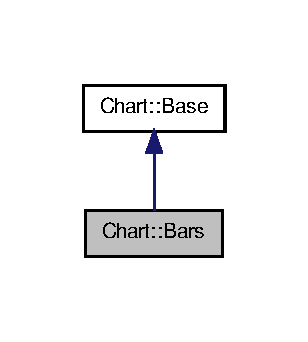
\includegraphics[width=148pt]{classChart_1_1Bars__inherit__graph}
\end{center}
\end{figure}


Collaboration diagram for Chart::Bars:\nopagebreak
\begin{figure}[H]
\begin{center}
\leavevmode
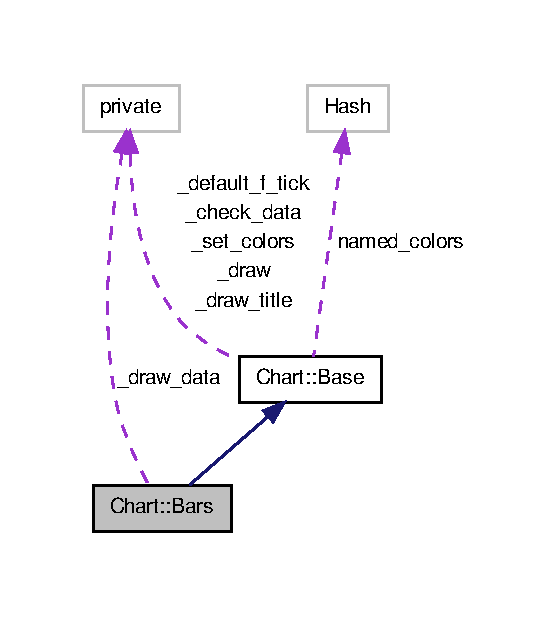
\includegraphics[width=303pt]{classChart_1_1Bars__coll__graph}
\end{center}
\end{figure}
\subsection*{Private Object Methods}
\label{_amgrp57eb0ba2c0003ce1a95a820bfa03b4b4}
 \begin{DoxyCompactItemize}
\item 
private \hyperlink{classChart_1_1Bars_ac15f867b92bbe0edcf3d971dc3a81812}{\_\-draw\_\-data}
\begin{DoxyCompactList}\small\item\em finally get around to plotting the data for (vertical) bars \item\end{DoxyCompactList}\end{DoxyCompactItemize}


\subsection{Detailed Description}
\hyperlink{classChart_1_1Bars}{Bars} class provides all functions which are specific to vertical bars. 

\subsection{Member Data Documentation}
\hypertarget{classChart_1_1Bars_ac15f867b92bbe0edcf3d971dc3a81812}{
\index{Chart::Bars@{Chart::Bars}!\_\-draw\_\-data@{\_\-draw\_\-data}}
\index{\_\-draw\_\-data@{\_\-draw\_\-data}!Chart::Bars@{Chart::Bars}}
\subsubsection[{\_\-draw\_\-data}]{\setlength{\rightskip}{0pt plus 5cm}private {\bf Chart::Bars::\_\-draw\_\-data}}}
\label{classChart_1_1Bars_ac15f867b92bbe0edcf3d971dc3a81812}


finally get around to plotting the data for (vertical) bars 



The documentation for this class was generated from the following file:\begin{DoxyCompactItemize}
\item 
Chart/\hyperlink{Bars_8pm}{Bars.pm}\end{DoxyCompactItemize}

\hypertarget{classChart_1_1Base}{
\section{Chart::Base Class Reference}
\label{classChart_1_1Base}\index{Chart::Base@{Chart::Base}}
}


\hyperlink{classChart_1_1Base}{Base} class for Chart; all other classes derived from here.  




Inheritance diagram for Chart::Base:\nopagebreak
\begin{figure}[H]
\begin{center}
\leavevmode
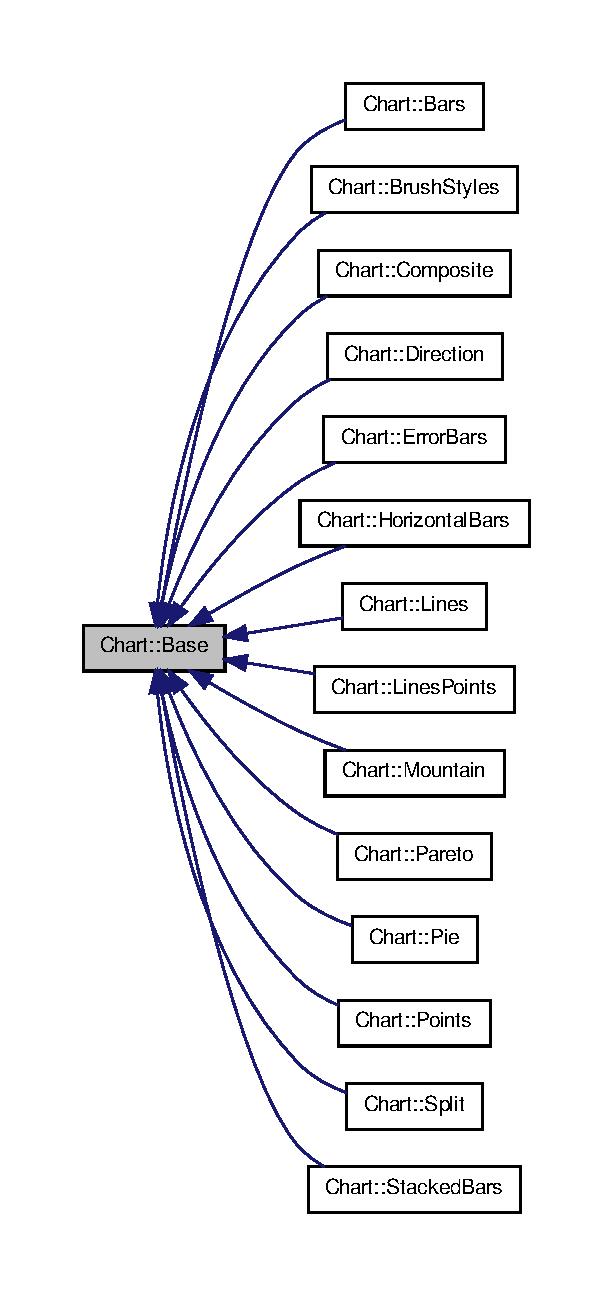
\includegraphics[height=600pt]{classChart_1_1Base__inherit__graph}
\end{center}
\end{figure}


Collaboration diagram for Chart::Base:\nopagebreak
\begin{figure}[H]
\begin{center}
\leavevmode
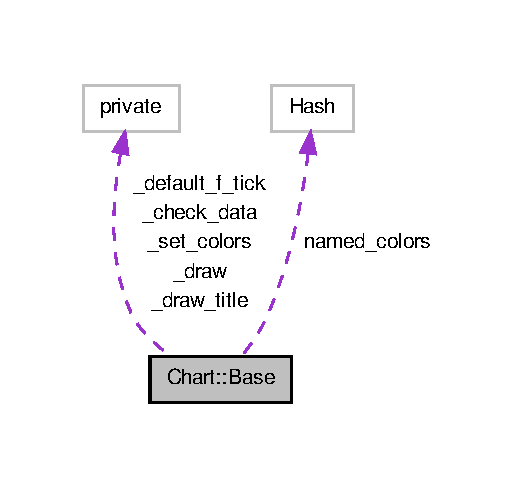
\includegraphics[width=288pt]{classChart_1_1Base__coll__graph}
\end{center}
\end{figure}
\subsection*{Public Attributes}
\begin{DoxyCompactItemize}
\item 
Hash \hyperlink{classChart_1_1Base_a38c2792df08724efa7c4e1b9194cbe6e}{named\_\-colors}
\begin{DoxyCompactList}\small\item\em RGB values of named colors. \item\end{DoxyCompactList}\end{DoxyCompactItemize}
\subsection*{Private Functions}
\label{_amgrp8d29cff216bafa3117e21883ea7c6b5f}
 \begin{DoxyCompactItemize}
\item 
private int \hyperlink{classChart_1_1Base_a13296be5b92a9880851977fe0abfdf01}{\_\-check\_\-data}
\begin{DoxyCompactList}\small\item\em Check the internal data to be displayed. \item\end{DoxyCompactList}\item 
private int \hyperlink{classChart_1_1Base_ab021c0dceb1ae55e1697bbee667480fa}{\_\-draw}
\begin{DoxyCompactList}\small\item\em Plot the chart to the gd object\par
 Calls: \item\end{DoxyCompactList}\item 
private int \hyperlink{classChart_1_1Base_addecc110eb46a126acaad69e113d06ea}{\_\-set\_\-colors}
\begin{DoxyCompactList}\small\item\em specify my colors \item\end{DoxyCompactList}\item 
private int \hyperlink{classChart_1_1Base_a14098e898b9f9b5dca8d7a39ab9d4d57}{\_\-color\_\-role\_\-to\_\-index}
\begin{DoxyCompactList}\small\item\em return a (list of) color index(es) corresponding to the (list of) role(s) \item\end{DoxyCompactList}\item 
private int \hyperlink{classChart_1_1Base_a2c02f66668131d6567338965e821d87a}{\_\-brushStyles\_\-of\_\-roles}
\begin{DoxyCompactList}\small\item\em return a (list of) brushStyles corresponding to the (list of) role(s) \item\end{DoxyCompactList}\item 
private int \hyperlink{classChart_1_1Base_aa3467472a4c4a598c5a2f64de8c438c1}{\_\-draw\_\-title}
\begin{DoxyCompactList}\small\item\em draw the title for the chart \item\end{DoxyCompactList}\item 
private int \hyperlink{classChart_1_1Base_a060d522a2f0240cad4c746891d488f80}{\_\-default\_\-f\_\-tick}
\begin{DoxyCompactList}\small\item\em default tick conversion function This function is pointed to be \$self-\/$>$\{f\_\-x\_\-tick\} resp. \item\end{DoxyCompactList}\item 
private float \hyperlink{classChart_1_1Base_a1f3ae34864bf296fafcab63416926b83}{\_\-xyRatio}
\begin{DoxyCompactList}\small\item\em Get ratio width\_\-x/width\_\-y. \item\end{DoxyCompactList}\item 
private float \hyperlink{classChart_1_1Base_ac21e93fb6498ea3137e15fd348e7b9ff}{\_\-xPixelInReal}
\begin{DoxyCompactList}\small\item\em Get witdh of one Pixel in real coordinates in x-\/direction. \item\end{DoxyCompactList}\item 
private float \hyperlink{classChart_1_1Base_afe24ee8f28c900069e65ddd666a242ff}{\_\-yPixelInReal}
\begin{DoxyCompactList}\small\item\em Get witdh of one Pixel in real coordinates in y-\/direction. \item\end{DoxyCompactList}\item 
private int \hyperlink{classChart_1_1Base_a0803aa94dabfc982195cab15392ba7bc}{\_\-init} (scalar x, scalar y)
\begin{DoxyCompactList}\small\item\em Initialize all default options here. \item\end{DoxyCompactList}\item 
private int \hyperlink{classChart_1_1Base_ac704c89b5b4b3f3f0e6fa35d6c5ca6c3}{\_\-copy\_\-data} (scalar extern\_\-ref)
\begin{DoxyCompactList}\small\item\em Copy external data via a reference to internal memory. \item\end{DoxyCompactList}\item 
private array \hyperlink{classChart_1_1Base_a6a97b446c6c2f646dddd7f2a0076ba2e}{\_\-color\_\-spec\_\-to\_\-rgb} (scalar role, scalar spec)
\begin{DoxyCompactList}\small\item\em Return an array (list of) rgb values for spec. \item\end{DoxyCompactList}\item 
private int \hyperlink{classChart_1_1Base_afd4f3ee3925d1e765e099c80e6c98da7}{\_\-draw\_\-sub\_\-title} ()
\begin{DoxyCompactList}\small\item\em draw the sub-\/title for the chart \item\end{DoxyCompactList}\item 
private int \hyperlink{classChart_1_1Base_ade88df5ecdc74e50ea683b63424ba84a}{\_\-sort\_\-data} ()
\begin{DoxyCompactList}\small\item\em sort the data nicely (mostly for the pareto charts and xy-\/plots) \item\end{DoxyCompactList}\item 
private int \hyperlink{classChart_1_1Base_a694b293ee3d92e706b1743cb1fa9d09d}{\_\-find\_\-x\_\-scale} ()
\begin{DoxyCompactList}\small\item\em For a xy-\/plot do the same for the x values, as '\_\-find\_\-y\_\-scale' does for the y values! \item\end{DoxyCompactList}\item 
private int \hyperlink{classChart_1_1Base_acb2fe91b2d57e43d84b1bc6f092ac68d}{\_\-find\_\-y\_\-scale} ()
\begin{DoxyCompactList}\small\item\em find good values for the minimum and maximum y-\/value on the chart \item\end{DoxyCompactList}\item 
private \hyperlink{classChart_1_1Base_a23f7394cb8c7bbe6a5d0e05582e038c9}{\_\-calcTickInterval} (scalar dataset\_\-min, scalar dataset\_\-max, scalar flag\_\-fixed\_\-min, scalar flag\_\-fixed\_\-max, scalar minTicks, scalar maxTicks)
\begin{DoxyCompactList}\small\item\em Calculate the Interval between ticks in y direction. \item\end{DoxyCompactList}\item 
private int \hyperlink{classChart_1_1Base_abc810d13339a6b0ab2f08ff8a96b82cb}{\_\-calcXTickInterval} (scalar min, scalar max, scalar minF, scalar maxF, scalar minTicks, scalar maxTicks)
\begin{DoxyCompactList}\small\item\em Calculate the Interval between ticks in x direction. \item\end{DoxyCompactList}\item 
private int \hyperlink{classChart_1_1Base_afb289639a7016adabc1cb03ae7851269}{\_\-countTicks} (scalar min, scalar max, scalar interval)
\begin{DoxyCompactList}\small\item\em Works out how many ticks would be displayed at that interval. \item\end{DoxyCompactList}\item 
private int \hyperlink{classChart_1_1Base_afaa4e9e29bc7fb9df56e9c7cd168e79b}{\_\-round2Tick} (scalar input, scalar interval, scalar roundUP)
\begin{DoxyCompactList}\small\item\em Rounds up or down to the next tick of interval size. \item\end{DoxyCompactList}\item 
private array \hyperlink{classChart_1_1Base_ab1f985ad443c2f1d1bf3ef86e9382346}{\_\-sepFP} (scalar num)
\begin{DoxyCompactList}\small\item\em Seperates a number into it's base 10 floating point exponent \& mantisa. \item\end{DoxyCompactList}\item 
private array \hyperlink{classChart_1_1Base_ad28e18fc86eebc6846785580977532ca}{\_\-find\_\-y\_\-range} ()
\begin{DoxyCompactList}\small\item\em Find minimum and maximum value of y data sets. \item\end{DoxyCompactList}\item 
private array \hyperlink{classChart_1_1Base_ab5b79dbb6f086902396bf5fd4c2248ef}{\_\-find\_\-x\_\-range} ()
\begin{DoxyCompactList}\small\item\em Find minimum and maximum value of x data sets. \item\end{DoxyCompactList}\item 
private int \hyperlink{classChart_1_1Base_aa13b0e86a933ce6b865c098fd0bdb37d}{\_\-plot} ()
\begin{DoxyCompactList}\small\item\em main sub that controls all the plotting of the actual chart \item\end{DoxyCompactList}\item 
private int \hyperlink{classChart_1_1Base_a530e742ca18ce2e89f177d367964277f}{\_\-draw\_\-legend} ()
\begin{DoxyCompactList}\small\item\em let the user know what all the pretty colors mean. \item\end{DoxyCompactList}\item 
private int \hyperlink{classChart_1_1Base_a863d96ec45b7fbd5ff05194f4eb827d0}{\_\-draw\_\-bottom\_\-legend} ()
\begin{DoxyCompactList}\small\item\em put the legend on the bottom of the chart \item\end{DoxyCompactList}\item 
private int \hyperlink{classChart_1_1Base_a39f25b556f2d82e176fc6b0ccfc6da17}{\_\-draw\_\-right\_\-legend} ()
\begin{DoxyCompactList}\small\item\em put the legend on the right of the chart \item\end{DoxyCompactList}\item 
private int \hyperlink{classChart_1_1Base_a2f3f15efadc46484126c94780748a534}{\_\-draw\_\-top\_\-legend} ()
\begin{DoxyCompactList}\small\item\em put the legend on top of the chart \item\end{DoxyCompactList}\item 
private int \hyperlink{classChart_1_1Base_a39bad67aecd83bf523bc27d397256480}{\_\-draw\_\-left\_\-legend} ()
\begin{DoxyCompactList}\small\item\em put the legend on the left of the chart \item\end{DoxyCompactList}\item 
private int \hyperlink{classChart_1_1Base_a2ec9e89bd6719e178877577a72750cb7}{\_\-draw\_\-none\_\-legend} ()
\begin{DoxyCompactList}\small\item\em no legend to draw. \item\end{DoxyCompactList}\item 
private int \hyperlink{classChart_1_1Base_a5ad71ca4e51c7d4876561737f048a6e7}{\_\-draw\_\-x\_\-label} ()
\begin{DoxyCompactList}\small\item\em draw the label for the x-\/axis \item\end{DoxyCompactList}\item 
private int \hyperlink{classChart_1_1Base_a6aafcea3c04d6a030a29892f04b25c1f}{\_\-draw\_\-y\_\-label} ()
\begin{DoxyCompactList}\small\item\em draw the label for the y-\/axis \item\end{DoxyCompactList}\item 
private int \hyperlink{classChart_1_1Base_a26f0a0f81ae5e6082c2e7f7c00981dac}{\_\-draw\_\-ticks} ()
\begin{DoxyCompactList}\small\item\em draw the ticks and tick labels \item\end{DoxyCompactList}\item 
private int \hyperlink{classChart_1_1Base_a4f10e76a428b6b09c7ac17a8d8212701}{\_\-draw\_\-x\_\-number\_\-ticks} ()
\begin{DoxyCompactList}\small\item\em draw the ticks and tick labels \item\end{DoxyCompactList}\item 
private int \hyperlink{classChart_1_1Base_a64a81b266a528e24e5547ac504c1fc78}{\_\-draw\_\-x\_\-ticks} ()
\begin{DoxyCompactList}\small\item\em draw the x-\/ticks and their labels \item\end{DoxyCompactList}\item 
private int \hyperlink{classChart_1_1Base_a46852297ab12aaf10546e63dd7eab462}{\_\-draw\_\-y\_\-ticks} ()
\begin{DoxyCompactList}\small\item\em draw the y-\/ticks and their labels \item\end{DoxyCompactList}\item 
private int \hyperlink{classChart_1_1Base_a8bae7e38a6e77c0696f2ef8b06791caa}{\_\-grey\_\-background} ()
\begin{DoxyCompactList}\small\item\em put a grey background on the plot of the data itself \item\end{DoxyCompactList}\item 
private int \hyperlink{classChart_1_1Base_a379e60b338fb8858ce705bdc0e5630fb}{\_\-draw\_\-grid\_\-lines} ()
\begin{DoxyCompactList}\small\item\em draw grid\_\-lines \item\end{DoxyCompactList}\item 
private int \hyperlink{classChart_1_1Base_afb41d27247195ea502c6f5a2d8e21eb6}{\_\-draw\_\-x\_\-grid\_\-lines} ()
\begin{DoxyCompactList}\small\item\em draw grid\_\-lines for x \item\end{DoxyCompactList}\item 
private int \hyperlink{classChart_1_1Base_aac178efe7b3c275cd18fe3c86b4d7a6f}{\_\-draw\_\-y\_\-grid\_\-lines} ()
\begin{DoxyCompactList}\small\item\em draw grid\_\-lines for y \item\end{DoxyCompactList}\item 
private int \hyperlink{classChart_1_1Base_af174cccca9ebbc23f588b6587e88fa1b}{\_\-draw\_\-y2\_\-grid\_\-lines} ()
\begin{DoxyCompactList}\small\item\em draw grid\_\-lines for y \item\end{DoxyCompactList}\item 
private int \hyperlink{classChart_1_1Base_ab86fa8ba6e10d109bd155bfefdb42ebf}{\_\-prepare\_\-brush} (scalar color, scalar type, scalar role)
\begin{DoxyCompactList}\small\item\em prepare brush \item\end{DoxyCompactList}\end{DoxyCompactItemize}
\subsection*{Public Class Methods}
\label{_amgrp76489900c371cf7d2ca502e43fa26e8e}
 \begin{DoxyCompactItemize}
\item 
object \hyperlink{classChart_1_1Base_a73931fdf090999a07299c1b42d23ae9d}{new} ()
\begin{DoxyCompactList}\small\item\em Standard normal constructor.\par
 Calls. \item\end{DoxyCompactList}\end{DoxyCompactItemize}
\subsection*{Public Object Methods}
\label{_amgrpfb74d91261823cc595bbeff1eff2b9d5}
 \begin{DoxyCompactItemize}
\item 
int \hyperlink{classChart_1_1Base_aadd99033eae9eab891cc2abdf7e4b74d}{set} (hash opts)
\begin{DoxyCompactList}\small\item\em Set all options. \item\end{DoxyCompactList}\item 
hash \hyperlink{classChart_1_1Base_a91b33c2a7d570aac658b2660a4d7b809}{getopts} ()
\begin{DoxyCompactList}\small\item\em get all options \item\end{DoxyCompactList}\item 
int \hyperlink{classChart_1_1Base_ac68c2d5654211e9e5c36674324fe0451}{add\_\-pt} (list data)
\begin{DoxyCompactList}\small\item\em Graph API\par
 Add one dataset (as a list) to the dataref. \item\end{DoxyCompactList}\item 
\hyperlink{classChart_1_1Base_a080e4b93239edf6886745c59506c14e5}{add\_\-pt} ($\backslash$list data)
\begin{DoxyCompactList}\small\item\em Graph API\par
 Add one dataset (as a reference to a list) to the dataref via. \item\end{DoxyCompactList}\item 
int \hyperlink{classChart_1_1Base_a43dcf87aa2b9fd362ba104923c3f3d51}{add\_\-dataset} (list data)
\begin{DoxyCompactList}\small\item\em Graph API\par
 Add many datasets (implemented as a list) to the dataref,. \item\end{DoxyCompactList}\item 
int \hyperlink{classChart_1_1Base_aa56e6de915dcdc29d00f66d9326b6503}{add\_\-dataset} ($\backslash$list data)
\begin{DoxyCompactList}\small\item\em Graph API\par
 Add many datasets (implemented as a references to alist) to the dataref,. \item\end{DoxyCompactList}\item 
int \hyperlink{classChart_1_1Base_a57eedac06ec67f93222bbe1a2930b606}{add\_\-datafile} (scalar filename, scalar format)
\begin{DoxyCompactList}\small\item\em Graph API\par
 it's also possible to add a complete datafile\par
 Uses. \item\end{DoxyCompactList}\item 
int \hyperlink{classChart_1_1Base_a99372014f79c259968b77c93eaddaf1a}{clear\_\-data} ()
\begin{DoxyCompactList}\small\item\em Clear Graph API (by undefining 'dataref'. \item\end{DoxyCompactList}\item 
arrayref \hyperlink{classChart_1_1Base_abafa3dfccde44d267a6aea07ad2a1274}{get\_\-data} ()
\begin{DoxyCompactList}\small\item\em Get array of data of the last graph. \item\end{DoxyCompactList}\item 
int \hyperlink{classChart_1_1Base_ac6b44856256fb2aa1bb40ee716431028}{png} (scalar file, scalar dataref)
\begin{DoxyCompactList}\small\item\em Produce the graph of options set in png format. \item\end{DoxyCompactList}\item 
int \hyperlink{classChart_1_1Base_a887fdd48d80d348d6a38ad799356b0ec}{cgi\_\-png} (scalar dataref)
\begin{DoxyCompactList}\small\item\em Produce the graph of options set in png format to be directly written for CGI. \item\end{DoxyCompactList}\item 
int \hyperlink{classChart_1_1Base_ad6bc3855bdc31bc6e264e390f5e660c2}{scalar\_\-png} (scalar dataref)
\begin{DoxyCompactList}\small\item\em Produce the graph of options set in png format to be directly written for CGI. \item\end{DoxyCompactList}\item 
int \hyperlink{classChart_1_1Base_aa9791b8cc8b287fa966402574afaf03f}{jpeg} (scalar file, scalar dataref)
\begin{DoxyCompactList}\small\item\em Produce the graph of options set in JPG format to be directly plotted. \item\end{DoxyCompactList}\item 
int \hyperlink{classChart_1_1Base_a4bb21f030ba3e48a8a1086634595a9cf}{cgi\_\-jpeg} (scalar dataref)
\begin{DoxyCompactList}\small\item\em Produce the graph of options set in JPG format to be directly for CGI. \item\end{DoxyCompactList}\item 
int \hyperlink{classChart_1_1Base_ac5d9aee386bf811e2770574fba85ec66}{scalar\_\-jpeg} (scalar dataref)
\begin{DoxyCompactList}\small\item\em Produce the graph of options set in JPG format to be directly. \item\end{DoxyCompactList}\item 
int \hyperlink{classChart_1_1Base_aee48a95d2dbc344911ee9a4cba3b51b0}{make\_\-gd} (scalar dataref)
\begin{DoxyCompactList}\small\item\em Produce the graph of options set in GD format to be directly. \item\end{DoxyCompactList}\item 
\hyperlink{classChart_1_1Base_af9fec7910f7254177a81252a03a0f587}{imagemap\_\-dump} ()
\begin{DoxyCompactList}\small\item\em get the information to turn the chart into an imagemap \item\end{DoxyCompactList}\item 
\hyperlink{classChart_1_1Base_ae65cef86e6b2f279b9446b01a9bea088}{minimum} (list array)
\begin{DoxyCompactList}\small\item\em determine minimum of an array of values \item\end{DoxyCompactList}\item 
\hyperlink{classChart_1_1Base_a3dd0d7d961b05b92020c476958b8e0a0}{maximum} (list array)
\begin{DoxyCompactList}\small\item\em determine maximum of an array of values \item\end{DoxyCompactList}\item 
\hyperlink{classChart_1_1Base_a97d3b67d31850ded3a7406a18c464ec9}{arccos} (scalar a)
\begin{DoxyCompactList}\small\item\em Function arccos(a). \item\end{DoxyCompactList}\item 
\hyperlink{classChart_1_1Base_a7da994b0d4ecf66262b4119745e38123}{arcsin} (scalar a)
\begin{DoxyCompactList}\small\item\em Function arcsin(a). \item\end{DoxyCompactList}\item 
\hyperlink{classChart_1_1Base_a9687d15b6d69b6a950f2b545940e62cd}{true} (scalar b)
\begin{DoxyCompactList}\small\item\em determine true value of argument \item\end{DoxyCompactList}\item 
\hyperlink{classChart_1_1Base_a72935251f89ad5d823649db7e07a3103}{false} (scalar b)
\begin{DoxyCompactList}\small\item\em determine false value of argument \item\end{DoxyCompactList}\end{DoxyCompactItemize}


\subsection{Detailed Description}
\hyperlink{classChart_1_1Base}{Base} class for Chart; all other classes derived from here. \hyperlink{classChart_1_1Base}{Base} class from which all other classes are derived. This class provides all functions which are common for all classes 

\subsection{Member Function Documentation}
\hypertarget{classChart_1_1Base_a23f7394cb8c7bbe6a5d0e05582e038c9}{
\index{Chart::Base@{Chart::Base}!\_\-calcTickInterval@{\_\-calcTickInterval}}
\index{\_\-calcTickInterval@{\_\-calcTickInterval}!Chart::Base@{Chart::Base}}
\subsubsection[{\_\-calcTickInterval}]{\setlength{\rightskip}{0pt plus 5cm}private Chart::Base::\_\-calcTickInterval (
\begin{DoxyParamCaption}
\item[{scalar}]{ dataset\_\-min, }
\item[{scalar}]{ dataset\_\-max, }
\item[{scalar}]{ flag\_\-fixed\_\-min, }
\item[{scalar}]{ flag\_\-fixed\_\-max, }
\item[{scalar}]{ minTicks, }
\item[{scalar}]{ maxTicks}
\end{DoxyParamCaption}
)}}
\label{classChart_1_1Base_a23f7394cb8c7bbe6a5d0e05582e038c9}


Calculate the Interval between ticks in y direction. 

Calculate the Interval between ticks in y direction and compare the number of ticks to the user's given values min\_\-y\_\-ticks, max\_\-y\_\-ticks.


\begin{DoxyParams}{Parameters}
\item[\mbox{\tt[in]} {\em \$dataset\_\-min}]Minimal value in y direction \item[\mbox{\tt[in]} {\em \$dataset\_\-max}]Maximal value in y direction \item[\mbox{\tt[in]} {\em \$flag\_\-fixed\_\-min}]Indicator whether the dataset\_\-min value is fixed \item[\mbox{\tt[in]} {\em \$flag\_\-fixed\_\-max}]Indicator whether the dataset\_\-max value is fixed \item[\mbox{\tt[in]} {\em \$minTicks}]Minimal number of ticks wanted \item[\mbox{\tt[in]} {\em \$maxTicks}]Maximal number of ticks wanted \end{DoxyParams}
\begin{DoxyReturn}{Returns}
Array of (\$tickInterval, \$tickCount, \$pMin, \$pMax) 
\end{DoxyReturn}


Reimplemented in \hyperlink{classChart_1_1Direction_a6766001399b56ba88e61f7ca0db50922}{Chart::Direction}.

\hypertarget{classChart_1_1Base_abc810d13339a6b0ab2f08ff8a96b82cb}{
\index{Chart::Base@{Chart::Base}!\_\-calcXTickInterval@{\_\-calcXTickInterval}}
\index{\_\-calcXTickInterval@{\_\-calcXTickInterval}!Chart::Base@{Chart::Base}}
\subsubsection[{\_\-calcXTickInterval}]{\setlength{\rightskip}{0pt plus 5cm}private int Chart::Base::\_\-calcXTickInterval (
\begin{DoxyParamCaption}
\item[{scalar}]{ min, }
\item[{scalar}]{ max, }
\item[{scalar}]{ minF, }
\item[{scalar}]{ maxF, }
\item[{scalar}]{ minTicks, }
\item[{scalar}]{ maxTicks}
\end{DoxyParamCaption}
)}}
\label{classChart_1_1Base_abc810d13339a6b0ab2f08ff8a96b82cb}


Calculate the Interval between ticks in x direction. 

Calculate the Interval between ticks in x direction and compare the number of ticks to the user's given values minTicks, maxTicks.


\begin{DoxyParams}{Parameters}
\item[\mbox{\tt[in]} {\em \$min}]Minimal value of dataset in x direction \item[\mbox{\tt[in]} {\em \$max}]Maximal value of dataset in x direction \item[\mbox{\tt[in]} {\em \$minF}]Inddicator if those min value is fixed \item[\mbox{\tt[in]} {\em \$maxF}]Inddicator if those max value is fixed \item[\mbox{\tt[in]} {\em \$minTicks}]Minimal number of tick in x direction \item[\mbox{\tt[in]} {\em \$maxTicks}]Maximal number of tick in x direction \end{DoxyParams}
\begin{DoxyReturn}{Returns}
\$tickInterval, \$tickCount, \$pMin, \$pMax 
\end{DoxyReturn}
\hypertarget{classChart_1_1Base_a6a97b446c6c2f646dddd7f2a0076ba2e}{
\index{Chart::Base@{Chart::Base}!\_\-color\_\-spec\_\-to\_\-rgb@{\_\-color\_\-spec\_\-to\_\-rgb}}
\index{\_\-color\_\-spec\_\-to\_\-rgb@{\_\-color\_\-spec\_\-to\_\-rgb}!Chart::Base@{Chart::Base}}
\subsubsection[{\_\-color\_\-spec\_\-to\_\-rgb}]{\setlength{\rightskip}{0pt plus 5cm}private array Chart::Base::\_\-color\_\-spec\_\-to\_\-rgb (
\begin{DoxyParamCaption}
\item[{scalar}]{ role, }
\item[{scalar}]{ spec}
\end{DoxyParamCaption}
)}}
\label{classChart_1_1Base_a6a97b446c6c2f646dddd7f2a0076ba2e}


Return an array (list of) rgb values for spec. 


\begin{DoxyParams}{Parameters}
\item[\mbox{\tt[in]} {\em \$role}]name of a role \item[\mbox{\tt[in]} {\em \$spec}]\mbox{[}r,g,b\mbox{]} or name \end{DoxyParams}
\begin{DoxyReturn}{Returns}
array of rgb values as a list (i.e., @rgb) 
\end{DoxyReturn}
\hypertarget{classChart_1_1Base_ac704c89b5b4b3f3f0e6fa35d6c5ca6c3}{
\index{Chart::Base@{Chart::Base}!\_\-copy\_\-data@{\_\-copy\_\-data}}
\index{\_\-copy\_\-data@{\_\-copy\_\-data}!Chart::Base@{Chart::Base}}
\subsubsection[{\_\-copy\_\-data}]{\setlength{\rightskip}{0pt plus 5cm}private int Chart::Base::\_\-copy\_\-data (
\begin{DoxyParamCaption}
\item[{scalar}]{ extern\_\-ref}
\end{DoxyParamCaption}
)}}
\label{classChart_1_1Base_ac704c89b5b4b3f3f0e6fa35d6c5ca6c3}


Copy external data via a reference to internal memory. 

Remember the external reference.\par
 Therefore, this function can anly be called once! 
\begin{DoxyParams}{Parameters}
\item[{\em \$extern\_\-ref}]Reference to external data space \end{DoxyParams}
\hypertarget{classChart_1_1Base_afb289639a7016adabc1cb03ae7851269}{
\index{Chart::Base@{Chart::Base}!\_\-countTicks@{\_\-countTicks}}
\index{\_\-countTicks@{\_\-countTicks}!Chart::Base@{Chart::Base}}
\subsubsection[{\_\-countTicks}]{\setlength{\rightskip}{0pt plus 5cm}private int Chart::Base::\_\-countTicks (
\begin{DoxyParamCaption}
\item[{scalar}]{ min, }
\item[{scalar}]{ max, }
\item[{scalar}]{ interval}
\end{DoxyParamCaption}
)}}
\label{classChart_1_1Base_afb289639a7016adabc1cb03ae7851269}


Works out how many ticks would be displayed at that interval. 


\begin{DoxyParams}{Parameters}
\item[{\em \$min}]Minimal value \item[{\em \$max}]Maximal value \item[{\em \$interval}]value \end{DoxyParams}
\begin{DoxyReturn}{Returns}
(\$tickCount, \$minR, \$maxR)
\end{DoxyReturn}
e.g min=2, max=5, interval=1, result is 4 ticks.\par
 written by David Pottage of Tao Group.\par
 \$minR = \$self-\/$>$\_\-round2Tick( \$min, \$interval, -\/1);\par
 \$maxR = \$self-\/$>$\_\-round2Tick( \$max, \$interval, 1);\par
 \$tickCount = ( \$maxR/\$interval ) -\/ ( \$minR/\$interval ) +1; \hypertarget{classChart_1_1Base_a863d96ec45b7fbd5ff05194f4eb827d0}{
\index{Chart::Base@{Chart::Base}!\_\-draw\_\-bottom\_\-legend@{\_\-draw\_\-bottom\_\-legend}}
\index{\_\-draw\_\-bottom\_\-legend@{\_\-draw\_\-bottom\_\-legend}!Chart::Base@{Chart::Base}}
\subsubsection[{\_\-draw\_\-bottom\_\-legend}]{\setlength{\rightskip}{0pt plus 5cm}private int Chart::Base::\_\-draw\_\-bottom\_\-legend (
\begin{DoxyParamCaption}
{}
\end{DoxyParamCaption}
)}}
\label{classChart_1_1Base_a863d96ec45b7fbd5ff05194f4eb827d0}


put the legend on the bottom of the chart 

\begin{DoxyReturn}{Returns}
status 
\end{DoxyReturn}


Reimplemented in \hyperlink{classChart_1_1Composite_a91f9c46886e61ae81057a7489632f366}{Chart::Composite}.

\hypertarget{classChart_1_1Base_a379e60b338fb8858ce705bdc0e5630fb}{
\index{Chart::Base@{Chart::Base}!\_\-draw\_\-grid\_\-lines@{\_\-draw\_\-grid\_\-lines}}
\index{\_\-draw\_\-grid\_\-lines@{\_\-draw\_\-grid\_\-lines}!Chart::Base@{Chart::Base}}
\subsubsection[{\_\-draw\_\-grid\_\-lines}]{\setlength{\rightskip}{0pt plus 5cm}private int Chart::Base::\_\-draw\_\-grid\_\-lines (
\begin{DoxyParamCaption}
{}
\end{DoxyParamCaption}
)}}
\label{classChart_1_1Base_a379e60b338fb8858ce705bdc0e5630fb}


draw grid\_\-lines 

\begin{DoxyReturn}{Returns}
status 
\end{DoxyReturn}
\hypertarget{classChart_1_1Base_a39bad67aecd83bf523bc27d397256480}{
\index{Chart::Base@{Chart::Base}!\_\-draw\_\-left\_\-legend@{\_\-draw\_\-left\_\-legend}}
\index{\_\-draw\_\-left\_\-legend@{\_\-draw\_\-left\_\-legend}!Chart::Base@{Chart::Base}}
\subsubsection[{\_\-draw\_\-left\_\-legend}]{\setlength{\rightskip}{0pt plus 5cm}private int Chart::Base::\_\-draw\_\-left\_\-legend (
\begin{DoxyParamCaption}
{}
\end{DoxyParamCaption}
)}}
\label{classChart_1_1Base_a39bad67aecd83bf523bc27d397256480}


put the legend on the left of the chart 

\begin{DoxyReturn}{Returns}
status 
\end{DoxyReturn}


Reimplemented in \hyperlink{classChart_1_1Composite_aaf2a13312cf3fda279eb6b7e37188027}{Chart::Composite}.

\hypertarget{classChart_1_1Base_a530e742ca18ce2e89f177d367964277f}{
\index{Chart::Base@{Chart::Base}!\_\-draw\_\-legend@{\_\-draw\_\-legend}}
\index{\_\-draw\_\-legend@{\_\-draw\_\-legend}!Chart::Base@{Chart::Base}}
\subsubsection[{\_\-draw\_\-legend}]{\setlength{\rightskip}{0pt plus 5cm}private int Chart::Base::\_\-draw\_\-legend (
\begin{DoxyParamCaption}
{}
\end{DoxyParamCaption}
)}}
\label{classChart_1_1Base_a530e742ca18ce2e89f177d367964277f}


let the user know what all the pretty colors mean. 

\par
 The user define the position of the legend by setting option 'legend' to 'top', 'bottom', 'left', 'right' or 'none'. The legend is positioned at the defined place, respectively. \begin{DoxyReturn}{Returns}
status 
\end{DoxyReturn}


Reimplemented in \hyperlink{classChart_1_1Composite_afcfacbb3cf9fde5a3d9debd6daca3291}{Chart::Composite}, \hyperlink{classChart_1_1Direction_a47ab5b61307d24d038ae77e62e269099}{Chart::Direction}, and \hyperlink{classChart_1_1ErrorBars_a6e1e40b048bbc13bead8449c2b78750a}{Chart::ErrorBars}.

\hypertarget{classChart_1_1Base_a2ec9e89bd6719e178877577a72750cb7}{
\index{Chart::Base@{Chart::Base}!\_\-draw\_\-none\_\-legend@{\_\-draw\_\-none\_\-legend}}
\index{\_\-draw\_\-none\_\-legend@{\_\-draw\_\-none\_\-legend}!Chart::Base@{Chart::Base}}
\subsubsection[{\_\-draw\_\-none\_\-legend}]{\setlength{\rightskip}{0pt plus 5cm}private int Chart::Base::\_\-draw\_\-none\_\-legend (
\begin{DoxyParamCaption}
{}
\end{DoxyParamCaption}
)}}
\label{classChart_1_1Base_a2ec9e89bd6719e178877577a72750cb7}


no legend to draw. 

Just return in this case. This routine may be overwritten by subclasses. \begin{DoxyReturn}{Returns}
1 
\end{DoxyReturn}


Reimplemented in \hyperlink{classChart_1_1Composite_a1f58fe4c7a6db069a7f4e173ac76a961}{Chart::Composite}.

\hypertarget{classChart_1_1Base_a39f25b556f2d82e176fc6b0ccfc6da17}{
\index{Chart::Base@{Chart::Base}!\_\-draw\_\-right\_\-legend@{\_\-draw\_\-right\_\-legend}}
\index{\_\-draw\_\-right\_\-legend@{\_\-draw\_\-right\_\-legend}!Chart::Base@{Chart::Base}}
\subsubsection[{\_\-draw\_\-right\_\-legend}]{\setlength{\rightskip}{0pt plus 5cm}private int Chart::Base::\_\-draw\_\-right\_\-legend (
\begin{DoxyParamCaption}
{}
\end{DoxyParamCaption}
)}}
\label{classChart_1_1Base_a39f25b556f2d82e176fc6b0ccfc6da17}


put the legend on the right of the chart 

\begin{DoxyReturn}{Returns}
status 
\end{DoxyReturn}


Reimplemented in \hyperlink{classChart_1_1Composite_ae2376bb07ec85374f24b76ac0dbc813a}{Chart::Composite}.

\hypertarget{classChart_1_1Base_afd4f3ee3925d1e765e099c80e6c98da7}{
\index{Chart::Base@{Chart::Base}!\_\-draw\_\-sub\_\-title@{\_\-draw\_\-sub\_\-title}}
\index{\_\-draw\_\-sub\_\-title@{\_\-draw\_\-sub\_\-title}!Chart::Base@{Chart::Base}}
\subsubsection[{\_\-draw\_\-sub\_\-title}]{\setlength{\rightskip}{0pt plus 5cm}private int Chart::Base::\_\-draw\_\-sub\_\-title (
\begin{DoxyParamCaption}
{}
\end{DoxyParamCaption}
)}}
\label{classChart_1_1Base_afd4f3ee3925d1e765e099c80e6c98da7}


draw the sub-\/title for the chart 

\begin{DoxySeeAlso}{See also}
\hyperlink{classChart_1_1Base_aa3467472a4c4a598c5a2f64de8c438c1}{\_\-draw\_\-title}\par
 \hyperlink{classChart_1_1Base_afd4f3ee3925d1e765e099c80e6c98da7}{\_\-draw\_\-sub\_\-title()} is more or less obsolete as \hyperlink{classChart_1_1Base_aa3467472a4c4a598c5a2f64de8c438c1}{\_\-draw\_\-title()} does the same by writing more than one line as the title. Both use decreased width and height of the font by one. 
\end{DoxySeeAlso}
\begin{DoxyReturn}{Returns}
status 
\end{DoxyReturn}
\hypertarget{classChart_1_1Base_a26f0a0f81ae5e6082c2e7f7c00981dac}{
\index{Chart::Base@{Chart::Base}!\_\-draw\_\-ticks@{\_\-draw\_\-ticks}}
\index{\_\-draw\_\-ticks@{\_\-draw\_\-ticks}!Chart::Base@{Chart::Base}}
\subsubsection[{\_\-draw\_\-ticks}]{\setlength{\rightskip}{0pt plus 5cm}private int Chart::Base::\_\-draw\_\-ticks (
\begin{DoxyParamCaption}
{}
\end{DoxyParamCaption}
)}}
\label{classChart_1_1Base_a26f0a0f81ae5e6082c2e7f7c00981dac}


draw the ticks and tick labels 

\begin{DoxyReturn}{Returns}
status 
\end{DoxyReturn}


Reimplemented in \hyperlink{classChart_1_1Composite_a7851868c22518f010a467689cec79b93}{Chart::Composite}.

\hypertarget{classChart_1_1Base_a2f3f15efadc46484126c94780748a534}{
\index{Chart::Base@{Chart::Base}!\_\-draw\_\-top\_\-legend@{\_\-draw\_\-top\_\-legend}}
\index{\_\-draw\_\-top\_\-legend@{\_\-draw\_\-top\_\-legend}!Chart::Base@{Chart::Base}}
\subsubsection[{\_\-draw\_\-top\_\-legend}]{\setlength{\rightskip}{0pt plus 5cm}private int Chart::Base::\_\-draw\_\-top\_\-legend (
\begin{DoxyParamCaption}
{}
\end{DoxyParamCaption}
)}}
\label{classChart_1_1Base_a2f3f15efadc46484126c94780748a534}


put the legend on top of the chart 

\begin{DoxyReturn}{Returns}
status 
\end{DoxyReturn}


Reimplemented in \hyperlink{classChart_1_1Composite_a844a6a68ef755e13236e013decf9cddf}{Chart::Composite}.

\hypertarget{classChart_1_1Base_afb41d27247195ea502c6f5a2d8e21eb6}{
\index{Chart::Base@{Chart::Base}!\_\-draw\_\-x\_\-grid\_\-lines@{\_\-draw\_\-x\_\-grid\_\-lines}}
\index{\_\-draw\_\-x\_\-grid\_\-lines@{\_\-draw\_\-x\_\-grid\_\-lines}!Chart::Base@{Chart::Base}}
\subsubsection[{\_\-draw\_\-x\_\-grid\_\-lines}]{\setlength{\rightskip}{0pt plus 5cm}private int Chart::Base::\_\-draw\_\-x\_\-grid\_\-lines (
\begin{DoxyParamCaption}
{}
\end{DoxyParamCaption}
)}}
\label{classChart_1_1Base_afb41d27247195ea502c6f5a2d8e21eb6}


draw grid\_\-lines for x 

\begin{DoxyReturn}{Returns}
status 
\end{DoxyReturn}
\hypertarget{classChart_1_1Base_a5ad71ca4e51c7d4876561737f048a6e7}{
\index{Chart::Base@{Chart::Base}!\_\-draw\_\-x\_\-label@{\_\-draw\_\-x\_\-label}}
\index{\_\-draw\_\-x\_\-label@{\_\-draw\_\-x\_\-label}!Chart::Base@{Chart::Base}}
\subsubsection[{\_\-draw\_\-x\_\-label}]{\setlength{\rightskip}{0pt plus 5cm}private int Chart::Base::\_\-draw\_\-x\_\-label (
\begin{DoxyParamCaption}
{}
\end{DoxyParamCaption}
)}}
\label{classChart_1_1Base_a5ad71ca4e51c7d4876561737f048a6e7}


draw the label for the x-\/axis 

Get font for labels\par
 Get the color of x\_\-label or text\par
 Get size of font\par
 and write x-\/Label

\begin{DoxyReturn}{Returns}
status 
\end{DoxyReturn}
\hypertarget{classChart_1_1Base_a4f10e76a428b6b09c7ac17a8d8212701}{
\index{Chart::Base@{Chart::Base}!\_\-draw\_\-x\_\-number\_\-ticks@{\_\-draw\_\-x\_\-number\_\-ticks}}
\index{\_\-draw\_\-x\_\-number\_\-ticks@{\_\-draw\_\-x\_\-number\_\-ticks}!Chart::Base@{Chart::Base}}
\subsubsection[{\_\-draw\_\-x\_\-number\_\-ticks}]{\setlength{\rightskip}{0pt plus 5cm}private int Chart::Base::\_\-draw\_\-x\_\-number\_\-ticks (
\begin{DoxyParamCaption}
{}
\end{DoxyParamCaption}
)}}
\label{classChart_1_1Base_a4f10e76a428b6b09c7ac17a8d8212701}


draw the ticks and tick labels 

\begin{DoxyReturn}{Returns}
status 
\end{DoxyReturn}
\hypertarget{classChart_1_1Base_a64a81b266a528e24e5547ac504c1fc78}{
\index{Chart::Base@{Chart::Base}!\_\-draw\_\-x\_\-ticks@{\_\-draw\_\-x\_\-ticks}}
\index{\_\-draw\_\-x\_\-ticks@{\_\-draw\_\-x\_\-ticks}!Chart::Base@{Chart::Base}}
\subsubsection[{\_\-draw\_\-x\_\-ticks}]{\setlength{\rightskip}{0pt plus 5cm}private int Chart::Base::\_\-draw\_\-x\_\-ticks (
\begin{DoxyParamCaption}
{}
\end{DoxyParamCaption}
)}}
\label{classChart_1_1Base_a64a81b266a528e24e5547ac504c1fc78}


draw the x-\/ticks and their labels 

\begin{DoxyReturn}{Returns}
status 
\end{DoxyReturn}


Reimplemented in \hyperlink{classChart_1_1Composite_a346409df6cbd56dae5206294a8e9edcb}{Chart::Composite}, \hyperlink{classChart_1_1Direction_a4803bef9580feed235401ff290459cce}{Chart::Direction}, and \hyperlink{classChart_1_1HorizontalBars_aabe5236ec45ce98269d60ea17944e283}{Chart::HorizontalBars}.

\hypertarget{classChart_1_1Base_af174cccca9ebbc23f588b6587e88fa1b}{
\index{Chart::Base@{Chart::Base}!\_\-draw\_\-y2\_\-grid\_\-lines@{\_\-draw\_\-y2\_\-grid\_\-lines}}
\index{\_\-draw\_\-y2\_\-grid\_\-lines@{\_\-draw\_\-y2\_\-grid\_\-lines}!Chart::Base@{Chart::Base}}
\subsubsection[{\_\-draw\_\-y2\_\-grid\_\-lines}]{\setlength{\rightskip}{0pt plus 5cm}private int Chart::Base::\_\-draw\_\-y2\_\-grid\_\-lines (
\begin{DoxyParamCaption}
{}
\end{DoxyParamCaption}
)}}
\label{classChart_1_1Base_af174cccca9ebbc23f588b6587e88fa1b}


draw grid\_\-lines for y 

\begin{DoxyReturn}{Returns}
status 
\end{DoxyReturn}


Reimplemented in \hyperlink{classChart_1_1Composite_a37406d5ce28e2e8a0465eeff8bfd6911}{Chart::Composite}.

\hypertarget{classChart_1_1Base_aac178efe7b3c275cd18fe3c86b4d7a6f}{
\index{Chart::Base@{Chart::Base}!\_\-draw\_\-y\_\-grid\_\-lines@{\_\-draw\_\-y\_\-grid\_\-lines}}
\index{\_\-draw\_\-y\_\-grid\_\-lines@{\_\-draw\_\-y\_\-grid\_\-lines}!Chart::Base@{Chart::Base}}
\subsubsection[{\_\-draw\_\-y\_\-grid\_\-lines}]{\setlength{\rightskip}{0pt plus 5cm}private int Chart::Base::\_\-draw\_\-y\_\-grid\_\-lines (
\begin{DoxyParamCaption}
{}
\end{DoxyParamCaption}
)}}
\label{classChart_1_1Base_aac178efe7b3c275cd18fe3c86b4d7a6f}


draw grid\_\-lines for y 

\begin{DoxyReturn}{Returns}
status 
\end{DoxyReturn}


Reimplemented in \hyperlink{classChart_1_1Composite_a6a727845be209cb4d9cb825ab6c5ffb1}{Chart::Composite}.

\hypertarget{classChart_1_1Base_a6aafcea3c04d6a030a29892f04b25c1f}{
\index{Chart::Base@{Chart::Base}!\_\-draw\_\-y\_\-label@{\_\-draw\_\-y\_\-label}}
\index{\_\-draw\_\-y\_\-label@{\_\-draw\_\-y\_\-label}!Chart::Base@{Chart::Base}}
\subsubsection[{\_\-draw\_\-y\_\-label}]{\setlength{\rightskip}{0pt plus 5cm}private int Chart::Base::\_\-draw\_\-y\_\-label (
\begin{DoxyParamCaption}
{}
\end{DoxyParamCaption}
)}}
\label{classChart_1_1Base_a6aafcea3c04d6a030a29892f04b25c1f}


draw the label for the y-\/axis 

\begin{DoxyReturn}{Returns}
status 
\end{DoxyReturn}
\hypertarget{classChart_1_1Base_a46852297ab12aaf10546e63dd7eab462}{
\index{Chart::Base@{Chart::Base}!\_\-draw\_\-y\_\-ticks@{\_\-draw\_\-y\_\-ticks}}
\index{\_\-draw\_\-y\_\-ticks@{\_\-draw\_\-y\_\-ticks}!Chart::Base@{Chart::Base}}
\subsubsection[{\_\-draw\_\-y\_\-ticks}]{\setlength{\rightskip}{0pt plus 5cm}private int Chart::Base::\_\-draw\_\-y\_\-ticks (
\begin{DoxyParamCaption}
{}
\end{DoxyParamCaption}
)}}
\label{classChart_1_1Base_a46852297ab12aaf10546e63dd7eab462}


draw the y-\/ticks and their labels 

\begin{DoxyReturn}{Returns}
status 
\end{DoxyReturn}


Reimplemented in \hyperlink{classChart_1_1Composite_a62fd62f54c05506571d4603e5618af30}{Chart::Composite}, \hyperlink{classChart_1_1Direction_aae701e9961733ae43e068acbad3e139a}{Chart::Direction}, and \hyperlink{classChart_1_1HorizontalBars_afb085d5cca48ae94538f345945212a82}{Chart::HorizontalBars}.

\hypertarget{classChart_1_1Base_ab5b79dbb6f086902396bf5fd4c2248ef}{
\index{Chart::Base@{Chart::Base}!\_\-find\_\-x\_\-range@{\_\-find\_\-x\_\-range}}
\index{\_\-find\_\-x\_\-range@{\_\-find\_\-x\_\-range}!Chart::Base@{Chart::Base}}
\subsubsection[{\_\-find\_\-x\_\-range}]{\setlength{\rightskip}{0pt plus 5cm}private array Chart::Base::\_\-find\_\-x\_\-range (
\begin{DoxyParamCaption}
{}
\end{DoxyParamCaption}
)}}
\label{classChart_1_1Base_ab5b79dbb6f086902396bf5fd4c2248ef}


Find minimum and maximum value of x data sets. 

\begin{DoxyReturn}{Returns}
( min, max ) 
\end{DoxyReturn}
\hypertarget{classChart_1_1Base_a694b293ee3d92e706b1743cb1fa9d09d}{
\index{Chart::Base@{Chart::Base}!\_\-find\_\-x\_\-scale@{\_\-find\_\-x\_\-scale}}
\index{\_\-find\_\-x\_\-scale@{\_\-find\_\-x\_\-scale}!Chart::Base@{Chart::Base}}
\subsubsection[{\_\-find\_\-x\_\-scale}]{\setlength{\rightskip}{0pt plus 5cm}private int Chart::Base::\_\-find\_\-x\_\-scale (
\begin{DoxyParamCaption}
{}
\end{DoxyParamCaption}
)}}
\label{classChart_1_1Base_a694b293ee3d92e706b1743cb1fa9d09d}


For a xy-\/plot do the same for the x values, as '\_\-find\_\-y\_\-scale' does for the y values! 

\begin{DoxySeeAlso}{See also}
\hyperlink{classChart_1_1Base_acb2fe91b2d57e43d84b1bc6f092ac68d}{\_\-find\_\-y\_\-scale} 
\end{DoxySeeAlso}
\begin{DoxyReturn}{Returns}
status 
\end{DoxyReturn}
\hypertarget{classChart_1_1Base_ad28e18fc86eebc6846785580977532ca}{
\index{Chart::Base@{Chart::Base}!\_\-find\_\-y\_\-range@{\_\-find\_\-y\_\-range}}
\index{\_\-find\_\-y\_\-range@{\_\-find\_\-y\_\-range}!Chart::Base@{Chart::Base}}
\subsubsection[{\_\-find\_\-y\_\-range}]{\setlength{\rightskip}{0pt plus 5cm}private array Chart::Base::\_\-find\_\-y\_\-range (
\begin{DoxyParamCaption}
{}
\end{DoxyParamCaption}
)}}
\label{classChart_1_1Base_ad28e18fc86eebc6846785580977532ca}


Find minimum and maximum value of y data sets. 

\begin{DoxyReturn}{Returns}
( min, max, flag\_\-all\_\-integers ) 
\end{DoxyReturn}


Reimplemented in \hyperlink{classChart_1_1Direction_a8f408c9fa61c3ee5f87a19c1f42d94c7}{Chart::Direction}, \hyperlink{classChart_1_1ErrorBars_aa303b7b246e29f54626fecebfe6cf15c}{Chart::ErrorBars}, and \hyperlink{classChart_1_1Mountain_a1da3590b6cb7bc51b8c192e1141a6fa3}{Chart::Mountain}.

\hypertarget{classChart_1_1Base_acb2fe91b2d57e43d84b1bc6f092ac68d}{
\index{Chart::Base@{Chart::Base}!\_\-find\_\-y\_\-scale@{\_\-find\_\-y\_\-scale}}
\index{\_\-find\_\-y\_\-scale@{\_\-find\_\-y\_\-scale}!Chart::Base@{Chart::Base}}
\subsubsection[{\_\-find\_\-y\_\-scale}]{\setlength{\rightskip}{0pt plus 5cm}private int Chart::Base::\_\-find\_\-y\_\-scale (
\begin{DoxyParamCaption}
{}
\end{DoxyParamCaption}
)}}
\label{classChart_1_1Base_acb2fe91b2d57e43d84b1bc6f092ac68d}


find good values for the minimum and maximum y-\/value on the chart 

\begin{DoxyReturn}{Returns}
status
\end{DoxyReturn}
New version, re-\/written by David Pottage of Tao Group.\par
 This code is $\ast$AS IS$\ast$ and comes with $\ast$NO WARRANTY$\ast$\par


This Sub calculates correct values for the following class local variables, if they have not been set by the user.

max\_\-val, min\_\-val: The maximum and minimum values for the y axis.\par
 y\_\-ticks: The number of ticks to plot on the y scale, including the end points. e.g. If the scale runs from 0 to 50, with ticks every 10, y\_\-ticks will have the value of 6.\par
 y\_\-tick\_\-labels: An array of strings, each is a label for the y axis.\par
 y\_\-tick\_\-labels\_\-length: The length to allow for B tick labels. (How long is the longest?) 

Reimplemented in \hyperlink{classChart_1_1Direction_ad33ea739bd5ceb8b48809028c489f119}{Chart::Direction}, and \hyperlink{classChart_1_1HorizontalBars_acec45b0698c777d244fb6f6dd1202e20}{Chart::HorizontalBars}.

\hypertarget{classChart_1_1Base_a8bae7e38a6e77c0696f2ef8b06791caa}{
\index{Chart::Base@{Chart::Base}!\_\-grey\_\-background@{\_\-grey\_\-background}}
\index{\_\-grey\_\-background@{\_\-grey\_\-background}!Chart::Base@{Chart::Base}}
\subsubsection[{\_\-grey\_\-background}]{\setlength{\rightskip}{0pt plus 5cm}private int Chart::Base::\_\-grey\_\-background (
\begin{DoxyParamCaption}
{}
\end{DoxyParamCaption}
)}}
\label{classChart_1_1Base_a8bae7e38a6e77c0696f2ef8b06791caa}


put a grey background on the plot of the data itself 

\begin{DoxyReturn}{Returns}
status 
\end{DoxyReturn}
\hypertarget{classChart_1_1Base_a0803aa94dabfc982195cab15392ba7bc}{
\index{Chart::Base@{Chart::Base}!\_\-init@{\_\-init}}
\index{\_\-init@{\_\-init}!Chart::Base@{Chart::Base}}
\subsubsection[{\_\-init}]{\setlength{\rightskip}{0pt plus 5cm}private int Chart::Base::\_\-init (
\begin{DoxyParamCaption}
\item[{scalar}]{ x, }
\item[{scalar}]{ y}
\end{DoxyParamCaption}
)}}
\label{classChart_1_1Base_a0803aa94dabfc982195cab15392ba7bc}


Initialize all default options here. 


\begin{DoxyParams}{Parameters}
\item[\mbox{\tt[in]} {\em \$x}]Width of the final image in pixels (Default: 400) \item[\mbox{\tt[in]} {\em \$y}]Height of the final image in pixels (Default: 300) \end{DoxyParams}
\hypertarget{classChart_1_1Base_aa13b0e86a933ce6b865c098fd0bdb37d}{
\index{Chart::Base@{Chart::Base}!\_\-plot@{\_\-plot}}
\index{\_\-plot@{\_\-plot}!Chart::Base@{Chart::Base}}
\subsubsection[{\_\-plot}]{\setlength{\rightskip}{0pt plus 5cm}private int Chart::Base::\_\-plot (
\begin{DoxyParamCaption}
{}
\end{DoxyParamCaption}
)}}
\label{classChart_1_1Base_aa13b0e86a933ce6b865c098fd0bdb37d}


main sub that controls all the plotting of the actual chart 

\begin{DoxyReturn}{Returns}
status 
\end{DoxyReturn}
\hypertarget{classChart_1_1Base_ab86fa8ba6e10d109bd155bfefdb42ebf}{
\index{Chart::Base@{Chart::Base}!\_\-prepare\_\-brush@{\_\-prepare\_\-brush}}
\index{\_\-prepare\_\-brush@{\_\-prepare\_\-brush}!Chart::Base@{Chart::Base}}
\subsubsection[{\_\-prepare\_\-brush}]{\setlength{\rightskip}{0pt plus 5cm}private int Chart::Base::\_\-prepare\_\-brush (
\begin{DoxyParamCaption}
\item[{scalar}]{ color, }
\item[{scalar}]{ type, }
\item[{scalar}]{ role}
\end{DoxyParamCaption}
)}}
\label{classChart_1_1Base_ab86fa8ba6e10d109bd155bfefdb42ebf}


prepare brush 

set the gdBrush object to tick GD into drawing fat lines \& points of interesting shapes Needed by \char`\"{}Lines\char`\"{}, \char`\"{}Points\char`\"{} and \char`\"{}LinesPoints\char`\"{} All hacked up by Richard Dice $<$\href{mailto:rdice@pobox.com}{\tt rdice@pobox.com}$>$ Sunday 16 May 1999


\begin{DoxyParams}{Parameters}
\item[{\em \$color}]\item[{\em \$type}]'line','point' \item[{\em \$role}]\end{DoxyParams}
\begin{DoxyReturn}{Returns}
status 
\end{DoxyReturn}
\hypertarget{classChart_1_1Base_afaa4e9e29bc7fb9df56e9c7cd168e79b}{
\index{Chart::Base@{Chart::Base}!\_\-round2Tick@{\_\-round2Tick}}
\index{\_\-round2Tick@{\_\-round2Tick}!Chart::Base@{Chart::Base}}
\subsubsection[{\_\-round2Tick}]{\setlength{\rightskip}{0pt plus 5cm}private int Chart::Base::\_\-round2Tick (
\begin{DoxyParamCaption}
\item[{scalar}]{ input, }
\item[{scalar}]{ interval, }
\item[{scalar}]{ roundUP}
\end{DoxyParamCaption}
)}}
\label{classChart_1_1Base_afaa4e9e29bc7fb9df56e9c7cd168e79b}


Rounds up or down to the next tick of interval size. 

\$roundUP can be +1 or -\/1 to indicate if rounding should be up or down.\par
 written by David Pottage of Tao Group.


\begin{DoxyParams}{Parameters}
\item[{\em \$input}]\item[{\em \$interval}]\item[{\em \$roundUP}]\end{DoxyParams}
\begin{DoxyReturn}{Returns}
retN$\ast$interval 
\end{DoxyReturn}
\hypertarget{classChart_1_1Base_ab1f985ad443c2f1d1bf3ef86e9382346}{
\index{Chart::Base@{Chart::Base}!\_\-sepFP@{\_\-sepFP}}
\index{\_\-sepFP@{\_\-sepFP}!Chart::Base@{Chart::Base}}
\subsubsection[{\_\-sepFP}]{\setlength{\rightskip}{0pt plus 5cm}private array Chart::Base::\_\-sepFP (
\begin{DoxyParamCaption}
\item[{scalar}]{ num}
\end{DoxyParamCaption}
)}}
\label{classChart_1_1Base_ab1f985ad443c2f1d1bf3ef86e9382346}


Seperates a number into it's base 10 floating point exponent \& mantisa. 

written by David Pottage of Tao Group.


\begin{DoxyParams}{Parameters}
\item[{\em \$num}]Floating point number \end{DoxyParams}
\begin{DoxyReturn}{Returns}
( exponent, mantissa) 
\end{DoxyReturn}
\hypertarget{classChart_1_1Base_ade88df5ecdc74e50ea683b63424ba84a}{
\index{Chart::Base@{Chart::Base}!\_\-sort\_\-data@{\_\-sort\_\-data}}
\index{\_\-sort\_\-data@{\_\-sort\_\-data}!Chart::Base@{Chart::Base}}
\subsubsection[{\_\-sort\_\-data}]{\setlength{\rightskip}{0pt plus 5cm}private int Chart::Base::\_\-sort\_\-data (
\begin{DoxyParamCaption}
{}
\end{DoxyParamCaption}
)}}
\label{classChart_1_1Base_ade88df5ecdc74e50ea683b63424ba84a}


sort the data nicely (mostly for the pareto charts and xy-\/plots) 

\begin{DoxyReturn}{Returns}
status 
\end{DoxyReturn}
\hypertarget{classChart_1_1Base_a57eedac06ec67f93222bbe1a2930b606}{
\index{Chart::Base@{Chart::Base}!add\_\-datafile@{add\_\-datafile}}
\index{add\_\-datafile@{add\_\-datafile}!Chart::Base@{Chart::Base}}
\subsubsection[{add\_\-datafile}]{\setlength{\rightskip}{0pt plus 5cm}int Chart::Base::add\_\-datafile (
\begin{DoxyParamCaption}
\item[{scalar}]{ filename, }
\item[{scalar}]{ format}
\end{DoxyParamCaption}
)}}
\label{classChart_1_1Base_a57eedac06ec67f93222bbe1a2930b606}


Graph API\par
 it's also possible to add a complete datafile\par
 Uses. 

\begin{DoxySeeAlso}{See also}
\hyperlink{classChart_1_1Base_ac68c2d5654211e9e5c36674324fe0451}{add\_\-pt} 

\hyperlink{classChart_1_1Base_a43dcf87aa2b9fd362ba104923c3f3d51}{add\_\-dataset}
\end{DoxySeeAlso}

\begin{DoxyParams}{Parameters}
\item[\mbox{\tt[in]} {\em \$filename}]Name of file which contents is to be added \item[\mbox{\tt[in]} {\em \$format}]'pt' or 'set' to distiguish between function \hyperlink{classChart_1_1Base_ac68c2d5654211e9e5c36674324fe0451}{add\_\-pt()} in case of 'pt' or function \hyperlink{classChart_1_1Base_a43dcf87aa2b9fd362ba104923c3f3d51}{add\_\-dataset()} in case of 'set' \end{DoxyParams}
\hypertarget{classChart_1_1Base_aa56e6de915dcdc29d00f66d9326b6503}{
\index{Chart::Base@{Chart::Base}!add\_\-dataset@{add\_\-dataset}}
\index{add\_\-dataset@{add\_\-dataset}!Chart::Base@{Chart::Base}}
\subsubsection[{add\_\-dataset}]{\setlength{\rightskip}{0pt plus 5cm}int Chart::Base::add\_\-dataset (
\begin{DoxyParamCaption}
\item[{$\backslash$list}]{ data}
\end{DoxyParamCaption}
)}}
\label{classChart_1_1Base_aa56e6de915dcdc29d00f66d9326b6503}


Graph API\par
 Add many datasets (implemented as a references to alist) to the dataref,. 


\begin{DoxyParams}{Parameters}
\item[{\em $\backslash$@data}]Dataset (reference to a list) to add \end{DoxyParams}
\hypertarget{classChart_1_1Base_a43dcf87aa2b9fd362ba104923c3f3d51}{
\index{Chart::Base@{Chart::Base}!add\_\-dataset@{add\_\-dataset}}
\index{add\_\-dataset@{add\_\-dataset}!Chart::Base@{Chart::Base}}
\subsubsection[{add\_\-dataset}]{\setlength{\rightskip}{0pt plus 5cm}int Chart::Base::add\_\-dataset (
\begin{DoxyParamCaption}
\item[{list}]{ data}
\end{DoxyParamCaption}
)}}
\label{classChart_1_1Base_a43dcf87aa2b9fd362ba104923c3f3d51}


Graph API\par
 Add many datasets (implemented as a list) to the dataref,. 


\begin{DoxyParams}{Parameters}
\item[{\em @data}]Dataset (list) to add \end{DoxyParams}


Reimplemented in \hyperlink{classChart_1_1Direction_a50b338ce75f7e6ab339b5f587a4e933b}{Chart::Direction}.

\hypertarget{classChart_1_1Base_a080e4b93239edf6886745c59506c14e5}{
\index{Chart::Base@{Chart::Base}!add\_\-pt@{add\_\-pt}}
\index{add\_\-pt@{add\_\-pt}!Chart::Base@{Chart::Base}}
\subsubsection[{add\_\-pt}]{\setlength{\rightskip}{0pt plus 5cm}Chart::Base::add\_\-pt (
\begin{DoxyParamCaption}
\item[{$\backslash$list}]{ data}
\end{DoxyParamCaption}
)}}
\label{classChart_1_1Base_a080e4b93239edf6886745c59506c14e5}


Graph API\par
 Add one dataset (as a reference to a list) to the dataref via. 


\begin{DoxyPre}
for ( 0 .. \$data )
\{
   push $self->\{'dataref'\}->[$\_] \}, $data[$\_];
\}
\end{DoxyPre}



\begin{DoxyParams}{Parameters}
\item[{\em $\backslash$@data}]Dataset to add \end{DoxyParams}
\hypertarget{classChart_1_1Base_ac68c2d5654211e9e5c36674324fe0451}{
\index{Chart::Base@{Chart::Base}!add\_\-pt@{add\_\-pt}}
\index{add\_\-pt@{add\_\-pt}!Chart::Base@{Chart::Base}}
\subsubsection[{add\_\-pt}]{\setlength{\rightskip}{0pt plus 5cm}int Chart::Base::add\_\-pt (
\begin{DoxyParamCaption}
\item[{list}]{ data}
\end{DoxyParamCaption}
)}}
\label{classChart_1_1Base_ac68c2d5654211e9e5c36674324fe0451}


Graph API\par
 Add one dataset (as a list) to the dataref. 


\begin{DoxyParams}{Parameters}
\item[{\em @data}]Dataset to add \end{DoxyParams}
\hypertarget{classChart_1_1Base_a97d3b67d31850ded3a7406a18c464ec9}{
\index{Chart::Base@{Chart::Base}!arccos@{arccos}}
\index{arccos@{arccos}!Chart::Base@{Chart::Base}}
\subsubsection[{arccos}]{\setlength{\rightskip}{0pt plus 5cm}Chart::Base::arccos (
\begin{DoxyParamCaption}
\item[{scalar}]{ a}
\end{DoxyParamCaption}
)}}
\label{classChart_1_1Base_a97d3b67d31850ded3a7406a18c464ec9}


Function arccos(a). 


\begin{DoxyParams}{Parameters}
\item[{\em \$a}]Value \end{DoxyParams}
\begin{DoxyReturn}{Returns}
arccos(a) 
\end{DoxyReturn}
\hypertarget{classChart_1_1Base_a7da994b0d4ecf66262b4119745e38123}{
\index{Chart::Base@{Chart::Base}!arcsin@{arcsin}}
\index{arcsin@{arcsin}!Chart::Base@{Chart::Base}}
\subsubsection[{arcsin}]{\setlength{\rightskip}{0pt plus 5cm}Chart::Base::arcsin (
\begin{DoxyParamCaption}
\item[{scalar}]{ a}
\end{DoxyParamCaption}
)}}
\label{classChart_1_1Base_a7da994b0d4ecf66262b4119745e38123}


Function arcsin(a). 


\begin{DoxyParams}{Parameters}
\item[{\em \$a}]Value \end{DoxyParams}
\begin{DoxyReturn}{Returns}
arcsin(a) 
\end{DoxyReturn}
\hypertarget{classChart_1_1Base_a4bb21f030ba3e48a8a1086634595a9cf}{
\index{Chart::Base@{Chart::Base}!cgi\_\-jpeg@{cgi\_\-jpeg}}
\index{cgi\_\-jpeg@{cgi\_\-jpeg}!Chart::Base@{Chart::Base}}
\subsubsection[{cgi\_\-jpeg}]{\setlength{\rightskip}{0pt plus 5cm}int Chart::Base::cgi\_\-jpeg (
\begin{DoxyParamCaption}
\item[{scalar}]{ dataref}
\end{DoxyParamCaption}
)}}
\label{classChart_1_1Base_a4bb21f030ba3e48a8a1086634595a9cf}


Produce the graph of options set in JPG format to be directly for CGI. 

called after the options are set, this method invokes all my private methods to actually draw the chart and plot the data 
\begin{DoxyParams}{Parameters}
\item[{\em \$dataref}]\end{DoxyParams}
\begin{DoxyReturn}{Returns}
Status of the plot 
\end{DoxyReturn}
\hypertarget{classChart_1_1Base_a887fdd48d80d348d6a38ad799356b0ec}{
\index{Chart::Base@{Chart::Base}!cgi\_\-png@{cgi\_\-png}}
\index{cgi\_\-png@{cgi\_\-png}!Chart::Base@{Chart::Base}}
\subsubsection[{cgi\_\-png}]{\setlength{\rightskip}{0pt plus 5cm}int Chart::Base::cgi\_\-png (
\begin{DoxyParamCaption}
\item[{scalar}]{ dataref}
\end{DoxyParamCaption}
)}}
\label{classChart_1_1Base_a887fdd48d80d348d6a38ad799356b0ec}


Produce the graph of options set in png format to be directly written for CGI. 

called after the options are set, this method invokes all my private methods to actually draw the chart and plot the data 
\begin{DoxyParams}{Parameters}
\item[{\em \$dataref}]\end{DoxyParams}
\begin{DoxyReturn}{Returns}
Status of the plot 
\end{DoxyReturn}
\hypertarget{classChart_1_1Base_a99372014f79c259968b77c93eaddaf1a}{
\index{Chart::Base@{Chart::Base}!clear\_\-data@{clear\_\-data}}
\index{clear\_\-data@{clear\_\-data}!Chart::Base@{Chart::Base}}
\subsubsection[{clear\_\-data}]{\setlength{\rightskip}{0pt plus 5cm}int Chart::Base::clear\_\-data (
\begin{DoxyParamCaption}
{}
\end{DoxyParamCaption}
)}}
\label{classChart_1_1Base_a99372014f79c259968b77c93eaddaf1a}


Clear Graph API (by undefining 'dataref'. 

\begin{DoxyReturn}{Returns}
Status of function 
\end{DoxyReturn}
\hypertarget{classChart_1_1Base_a72935251f89ad5d823649db7e07a3103}{
\index{Chart::Base@{Chart::Base}!false@{false}}
\index{false@{false}!Chart::Base@{Chart::Base}}
\subsubsection[{false}]{\setlength{\rightskip}{0pt plus 5cm}Chart::Base::false (
\begin{DoxyParamCaption}
\item[{scalar}]{ b}
\end{DoxyParamCaption}
)}}
\label{classChart_1_1Base_a72935251f89ad5d823649db7e07a3103}


determine false value of argument 


\begin{DoxyParams}{Parameters}
\item[\mbox{\tt[in]} {\em \$b}]Bool value to check for true \end{DoxyParams}
\begin{DoxyReturn}{Returns}
1 if argument is equal to false, FALSE, 0, f, F or undefined 
\end{DoxyReturn}
\hypertarget{classChart_1_1Base_abafa3dfccde44d267a6aea07ad2a1274}{
\index{Chart::Base@{Chart::Base}!get\_\-data@{get\_\-data}}
\index{get\_\-data@{get\_\-data}!Chart::Base@{Chart::Base}}
\subsubsection[{get\_\-data}]{\setlength{\rightskip}{0pt plus 5cm}arrayref Chart::Base::get\_\-data (
\begin{DoxyParamCaption}
{}
\end{DoxyParamCaption}
)}}
\label{classChart_1_1Base_abafa3dfccde44d267a6aea07ad2a1274}


Get array of data of the last graph. 

\begin{DoxyReturn}{Returns}
Reference to data set of the last graph 
\end{DoxyReturn}
\hypertarget{classChart_1_1Base_a91b33c2a7d570aac658b2660a4d7b809}{
\index{Chart::Base@{Chart::Base}!getopts@{getopts}}
\index{getopts@{getopts}!Chart::Base@{Chart::Base}}
\subsubsection[{getopts}]{\setlength{\rightskip}{0pt plus 5cm}hash Chart::Base::getopts (
\begin{DoxyParamCaption}
{}
\end{DoxyParamCaption}
)}}
\label{classChart_1_1Base_a91b33c2a7d570aac658b2660a4d7b809}


get all options 

\begin{DoxyReturn}{Returns}
hash of all set options so far

set options as a hash 
\end{DoxyReturn}
\hypertarget{classChart_1_1Base_af9fec7910f7254177a81252a03a0f587}{
\index{Chart::Base@{Chart::Base}!imagemap\_\-dump@{imagemap\_\-dump}}
\index{imagemap\_\-dump@{imagemap\_\-dump}!Chart::Base@{Chart::Base}}
\subsubsection[{imagemap\_\-dump}]{\setlength{\rightskip}{0pt plus 5cm}Chart::Base::imagemap\_\-dump (
\begin{DoxyParamCaption}
{}
\end{DoxyParamCaption}
)}}
\label{classChart_1_1Base_af9fec7910f7254177a81252a03a0f587}


get the information to turn the chart into an imagemap 

\begin{DoxyReturn}{Returns}
Reference to an array of the image 
\end{DoxyReturn}


Reimplemented in \hyperlink{classChart_1_1Composite_ab8dbbeec3544f8e9b1b10486aa46459d}{Chart::Composite}.

\hypertarget{classChart_1_1Base_aa9791b8cc8b287fa966402574afaf03f}{
\index{Chart::Base@{Chart::Base}!jpeg@{jpeg}}
\index{jpeg@{jpeg}!Chart::Base@{Chart::Base}}
\subsubsection[{jpeg}]{\setlength{\rightskip}{0pt plus 5cm}int Chart::Base::jpeg (
\begin{DoxyParamCaption}
\item[{scalar}]{ file, }
\item[{scalar}]{ dataref}
\end{DoxyParamCaption}
)}}
\label{classChart_1_1Base_aa9791b8cc8b287fa966402574afaf03f}


Produce the graph of options set in JPG format to be directly plotted. 

\par


Called after the options are set, this method invokes all my private methods to actually draw the chart and plot the data. The output has the jpeg format in opposite to png format produced by \begin{DoxySeeAlso}{See also}
\hyperlink{classChart_1_1Base_ac6b44856256fb2aa1bb40ee716431028}{png}
\end{DoxySeeAlso}
Uses the following private functions:\par
 \begin{DoxySeeAlso}{See also}
\hyperlink{classChart_1_1Base_addecc110eb46a126acaad69e113d06ea}{\_\-set\_\-colors} 

\hyperlink{classChart_1_1Base_ac704c89b5b4b3f3f0e6fa35d6c5ca6c3}{\_\-copy\_\-data} 

\hyperlink{classChart_1_1Base_a13296be5b92a9880851977fe0abfdf01}{\_\-check\_\-data} 

\hyperlink{classChart_1_1Base_ab021c0dceb1ae55e1697bbee667480fa}{\_\-draw}
\end{DoxySeeAlso}

\begin{DoxyParams}{Parameters}
\item[\mbox{\tt[in]} {\em \$file}]Name of file to write graph to \item[\mbox{\tt[in]} {\em \$dataref}]Reference to external data space \end{DoxyParams}
\begin{DoxyReturn}{Returns}
Status of the plot 
\end{DoxyReturn}
\hypertarget{classChart_1_1Base_aee48a95d2dbc344911ee9a4cba3b51b0}{
\index{Chart::Base@{Chart::Base}!make\_\-gd@{make\_\-gd}}
\index{make\_\-gd@{make\_\-gd}!Chart::Base@{Chart::Base}}
\subsubsection[{make\_\-gd}]{\setlength{\rightskip}{0pt plus 5cm}int Chart::Base::make\_\-gd (
\begin{DoxyParamCaption}
\item[{scalar}]{ dataref}
\end{DoxyParamCaption}
)}}
\label{classChart_1_1Base_aee48a95d2dbc344911ee9a4cba3b51b0}


Produce the graph of options set in GD format to be directly. 

called after the options are set, this method invokes all my private methods to actually draw the chart and plot the data 
\begin{DoxyParams}{Parameters}
\item[{\em \$dataref}]\end{DoxyParams}
\begin{DoxyReturn}{Returns}
Status of the plot 
\end{DoxyReturn}
\hypertarget{classChart_1_1Base_a3dd0d7d961b05b92020c476958b8e0a0}{
\index{Chart::Base@{Chart::Base}!maximum@{maximum}}
\index{maximum@{maximum}!Chart::Base@{Chart::Base}}
\subsubsection[{maximum}]{\setlength{\rightskip}{0pt plus 5cm}Chart::Base::maximum (
\begin{DoxyParamCaption}
\item[{list}]{ array}
\end{DoxyParamCaption}
)}}
\label{classChart_1_1Base_a3dd0d7d961b05b92020c476958b8e0a0}


determine maximum of an array of values 


\begin{DoxyParams}{Parameters}
\item[{\em @array}]List of numerical values \end{DoxyParams}
\begin{DoxyReturn}{Returns}
Maximal value of list of values 
\end{DoxyReturn}
\hypertarget{classChart_1_1Base_ae65cef86e6b2f279b9446b01a9bea088}{
\index{Chart::Base@{Chart::Base}!minimum@{minimum}}
\index{minimum@{minimum}!Chart::Base@{Chart::Base}}
\subsubsection[{minimum}]{\setlength{\rightskip}{0pt plus 5cm}Chart::Base::minimum (
\begin{DoxyParamCaption}
\item[{list}]{ array}
\end{DoxyParamCaption}
)}}
\label{classChart_1_1Base_ae65cef86e6b2f279b9446b01a9bea088}


determine minimum of an array of values 


\begin{DoxyParams}{Parameters}
\item[{\em @array}]List of numerical values \end{DoxyParams}
\begin{DoxyReturn}{Returns}
Minimal value of list of values 
\end{DoxyReturn}
\hypertarget{classChart_1_1Base_a73931fdf090999a07299c1b42d23ae9d}{
\index{Chart::Base@{Chart::Base}!new@{new}}
\index{new@{new}!Chart::Base@{Chart::Base}}
\subsubsection[{new}]{\setlength{\rightskip}{0pt plus 5cm}object Chart::Base::new (
\begin{DoxyParamCaption}
{}
\end{DoxyParamCaption}
)}}
\label{classChart_1_1Base_a73931fdf090999a07299c1b42d23ae9d}


Standard normal constructor.\par
 Calls. 

\begin{DoxyReturn}{Returns}
A new object.
\end{DoxyReturn}
\begin{DoxySeeAlso}{See also}
\hyperlink{classChart_1_1Base_a0803aa94dabfc982195cab15392ba7bc}{\_\-init} 
\end{DoxySeeAlso}
\hypertarget{classChart_1_1Base_ac6b44856256fb2aa1bb40ee716431028}{
\index{Chart::Base@{Chart::Base}!png@{png}}
\index{png@{png}!Chart::Base@{Chart::Base}}
\subsubsection[{png}]{\setlength{\rightskip}{0pt plus 5cm}int Chart::Base::png (
\begin{DoxyParamCaption}
\item[{scalar}]{ file, }
\item[{scalar}]{ dataref}
\end{DoxyParamCaption}
)}}
\label{classChart_1_1Base_ac6b44856256fb2aa1bb40ee716431028}


Produce the graph of options set in png format. 

called after the options are set, this method invokes all my private methods to actually draw the chart and plot the data \begin{DoxySeeAlso}{See also}
\hyperlink{classChart_1_1Base_addecc110eb46a126acaad69e113d06ea}{\_\-set\_\-colors} 

\hyperlink{classChart_1_1Base_ac704c89b5b4b3f3f0e6fa35d6c5ca6c3}{\_\-copy\_\-data} 

\hyperlink{classChart_1_1Base_a13296be5b92a9880851977fe0abfdf01}{\_\-check\_\-data} 

\hyperlink{classChart_1_1Base_ab021c0dceb1ae55e1697bbee667480fa}{\_\-draw} 
\end{DoxySeeAlso}

\begin{DoxyParams}{Parameters}
\item[\mbox{\tt[in]} {\em \$file}]Name of file to write graph to \item[\mbox{\tt[in]} {\em \$dataref}]Reference to external data space \end{DoxyParams}
\begin{DoxyReturn}{Returns}
Status of the plot 
\end{DoxyReturn}
\hypertarget{classChart_1_1Base_ac5d9aee386bf811e2770574fba85ec66}{
\index{Chart::Base@{Chart::Base}!scalar\_\-jpeg@{scalar\_\-jpeg}}
\index{scalar\_\-jpeg@{scalar\_\-jpeg}!Chart::Base@{Chart::Base}}
\subsubsection[{scalar\_\-jpeg}]{\setlength{\rightskip}{0pt plus 5cm}int Chart::Base::scalar\_\-jpeg (
\begin{DoxyParamCaption}
\item[{scalar}]{ dataref}
\end{DoxyParamCaption}
)}}
\label{classChart_1_1Base_ac5d9aee386bf811e2770574fba85ec66}


Produce the graph of options set in JPG format to be directly. 

called after the options are set, this method invokes all my private methods to actually draw the chart and plot the data 
\begin{DoxyParams}{Parameters}
\item[{\em \$dataref}]\end{DoxyParams}
\begin{DoxyReturn}{Returns}
Status of the plot 
\end{DoxyReturn}
\hypertarget{classChart_1_1Base_ad6bc3855bdc31bc6e264e390f5e660c2}{
\index{Chart::Base@{Chart::Base}!scalar\_\-png@{scalar\_\-png}}
\index{scalar\_\-png@{scalar\_\-png}!Chart::Base@{Chart::Base}}
\subsubsection[{scalar\_\-png}]{\setlength{\rightskip}{0pt plus 5cm}int Chart::Base::scalar\_\-png (
\begin{DoxyParamCaption}
\item[{scalar}]{ dataref}
\end{DoxyParamCaption}
)}}
\label{classChart_1_1Base_ad6bc3855bdc31bc6e264e390f5e660c2}


Produce the graph of options set in png format to be directly written for CGI. 

Called after the options are set, \par
 this method invokes all my private methods to actually draw the chart and plot the data 
\begin{DoxyParams}{Parameters}
\item[\mbox{\tt[in]} {\em \$dataref}]Reference to the data to be plotted \end{DoxyParams}
\begin{DoxyReturn}{Returns}
Status of the plot 
\end{DoxyReturn}
\hypertarget{classChart_1_1Base_aadd99033eae9eab891cc2abdf7e4b74d}{
\index{Chart::Base@{Chart::Base}!set@{set}}
\index{set@{set}!Chart::Base@{Chart::Base}}
\subsubsection[{set}]{\setlength{\rightskip}{0pt plus 5cm}int Chart::Base::set (
\begin{DoxyParamCaption}
\item[{hash}]{ opts}
\end{DoxyParamCaption}
)}}
\label{classChart_1_1Base_aadd99033eae9eab891cc2abdf7e4b74d}


Set all options. 

main method for customizing the chart, lets users specify values for different parameters\par
 The options are saved locally to be able to output them via \begin{DoxySeeAlso}{See also}
\hyperlink{classChart_1_1Base_a91b33c2a7d570aac658b2660a4d7b809}{getopts()}
\end{DoxySeeAlso}

\begin{DoxyParams}{Parameters}
\item[\mbox{\tt[in]} {\em \%opts}]Hash of options to the Chart \end{DoxyParams}
\begin{DoxyReturn}{Returns}
ok or croak 
\end{DoxyReturn}


Reimplemented in \hyperlink{classChart_1_1Composite_a00e87797c96ce57efc6b066cbe7d6333}{Chart::Composite}, and \hyperlink{classChart_1_1Direction_ab7104b48aa4219a995656088c121078d}{Chart::Direction}.

\hypertarget{classChart_1_1Base_a9687d15b6d69b6a950f2b545940e62cd}{
\index{Chart::Base@{Chart::Base}!true@{true}}
\index{true@{true}!Chart::Base@{Chart::Base}}
\subsubsection[{true}]{\setlength{\rightskip}{0pt plus 5cm}Chart::Base::true (
\begin{DoxyParamCaption}
\item[{scalar}]{ b}
\end{DoxyParamCaption}
)}}
\label{classChart_1_1Base_a9687d15b6d69b6a950f2b545940e62cd}


determine true value of argument 


\begin{DoxyParams}{Parameters}
\item[\mbox{\tt[in]} {\em \$b}]Bool value to check for true \end{DoxyParams}
\begin{DoxyReturn}{Returns}
1 if argument is equal to TRUE, true, 1, t, T, and defined 
\end{DoxyReturn}


\subsection{Member Data Documentation}
\hypertarget{classChart_1_1Base_a2c02f66668131d6567338965e821d87a}{
\index{Chart::Base@{Chart::Base}!\_\-brushStyles\_\-of\_\-roles@{\_\-brushStyles\_\-of\_\-roles}}
\index{\_\-brushStyles\_\-of\_\-roles@{\_\-brushStyles\_\-of\_\-roles}!Chart::Base@{Chart::Base}}
\subsubsection[{\_\-brushStyles\_\-of\_\-roles}]{\setlength{\rightskip}{0pt plus 5cm}private int {\bf Chart::Base::\_\-brushStyles\_\-of\_\-roles}}}
\label{classChart_1_1Base_a2c02f66668131d6567338965e821d87a}


return a (list of) brushStyles corresponding to the (list of) role(s) 


\begin{DoxyParams}{Parameters}
\item[{\em $\backslash$@list\_\-of\_\-roles}]List of roles \end{DoxyParams}
\begin{DoxyReturn}{Returns}
(list of) brushStyle(s) corresponding to the (list of) role(s) in @\_\-. 
\end{DoxyReturn}
\hypertarget{classChart_1_1Base_a13296be5b92a9880851977fe0abfdf01}{
\index{Chart::Base@{Chart::Base}!\_\-check\_\-data@{\_\-check\_\-data}}
\index{\_\-check\_\-data@{\_\-check\_\-data}!Chart::Base@{Chart::Base}}
\subsubsection[{\_\-check\_\-data}]{\setlength{\rightskip}{0pt plus 5cm}private int {\bf Chart::Base::\_\-check\_\-data}}}
\label{classChart_1_1Base_a13296be5b92a9880851977fe0abfdf01}


Check the internal data to be displayed. 

Make sure the data isn't really weird and collect some basic info about it\par
 Not logical data is 'carp'ed.\par
 \begin{DoxyReturn}{Returns}
status of check 
\end{DoxyReturn}


Reimplemented in \hyperlink{classChart_1_1Composite_a67af0ad77d0c1f4f74da434ceb9cf53c}{Chart::Composite}, and \hyperlink{classChart_1_1StackedBars_a8d772463780f75cc985ae890ad8a94d1}{Chart::StackedBars}.

\hypertarget{classChart_1_1Base_a14098e898b9f9b5dca8d7a39ab9d4d57}{
\index{Chart::Base@{Chart::Base}!\_\-color\_\-role\_\-to\_\-index@{\_\-color\_\-role\_\-to\_\-index}}
\index{\_\-color\_\-role\_\-to\_\-index@{\_\-color\_\-role\_\-to\_\-index}!Chart::Base@{Chart::Base}}
\subsubsection[{\_\-color\_\-role\_\-to\_\-index}]{\setlength{\rightskip}{0pt plus 5cm}private int {\bf Chart::Base::\_\-color\_\-role\_\-to\_\-index}}}
\label{classChart_1_1Base_a14098e898b9f9b5dca8d7a39ab9d4d57}


return a (list of) color index(es) corresponding to the (list of) role(s) 

wantarray is a special keyword which returns a flag indicating which context your subroutine has been called in. It will return one of three values.

\begin{DoxyItemize}
\item true: If your subroutine has been called in list context \item false: If your subroutine has been called in scalar context \item undef: If your subroutine has been called in void context\end{DoxyItemize}
\begin{DoxyReturn}{Returns}
a (list of) color index(es) corresponding to the (list of) role(s) in @\_\-. 
\end{DoxyReturn}
\hypertarget{classChart_1_1Base_a060d522a2f0240cad4c746891d488f80}{
\index{Chart::Base@{Chart::Base}!\_\-default\_\-f\_\-tick@{\_\-default\_\-f\_\-tick}}
\index{\_\-default\_\-f\_\-tick@{\_\-default\_\-f\_\-tick}!Chart::Base@{Chart::Base}}
\subsubsection[{\_\-default\_\-f\_\-tick}]{\setlength{\rightskip}{0pt plus 5cm}private int {\bf Chart::Base::\_\-default\_\-f\_\-tick}}}
\label{classChart_1_1Base_a060d522a2f0240cad4c746891d488f80}


default tick conversion function This function is pointed to be \$self-\/$>$\{f\_\-x\_\-tick\} resp. 

\$self-\/$>$\{f\_\-y\_\-tick\} if the user does not provide another function

\begin{DoxyReturn}{Returns}
status 
\end{DoxyReturn}
\hypertarget{classChart_1_1Base_ab021c0dceb1ae55e1697bbee667480fa}{
\index{Chart::Base@{Chart::Base}!\_\-draw@{\_\-draw}}
\index{\_\-draw@{\_\-draw}!Chart::Base@{Chart::Base}}
\subsubsection[{\_\-draw}]{\setlength{\rightskip}{0pt plus 5cm}private int {\bf Chart::Base::\_\-draw}}}
\label{classChart_1_1Base_ab021c0dceb1ae55e1697bbee667480fa}


Plot the chart to the gd object\par
 Calls: 

\begin{DoxySeeAlso}{See also}
\hyperlink{classChart_1_1Base_aa3467472a4c4a598c5a2f64de8c438c1}{\_\-draw\_\-title} 

\hyperlink{classChart_1_1Base_afd4f3ee3925d1e765e099c80e6c98da7}{\_\-draw\_\-sub\_\-title} 

\hyperlink{classChart_1_1Base_ade88df5ecdc74e50ea683b63424ba84a}{\_\-sort\_\-data} 

\hyperlink{classChart_1_1Base_aa13b0e86a933ce6b865c098fd0bdb37d}{\_\-plot}
\end{DoxySeeAlso}
\begin{DoxyReturn}{Returns}
status 
\end{DoxyReturn}
\hypertarget{classChart_1_1Base_aa3467472a4c4a598c5a2f64de8c438c1}{
\index{Chart::Base@{Chart::Base}!\_\-draw\_\-title@{\_\-draw\_\-title}}
\index{\_\-draw\_\-title@{\_\-draw\_\-title}!Chart::Base@{Chart::Base}}
\subsubsection[{\_\-draw\_\-title}]{\setlength{\rightskip}{0pt plus 5cm}private int {\bf Chart::Base::\_\-draw\_\-title}}}
\label{classChart_1_1Base_aa3467472a4c4a598c5a2f64de8c438c1}


draw the title for the chart 

The title was defined by the user in set('title' =$>$ ....)\par
 The user may define some title lines by separating them via character '$\backslash$n';\par
 The used font is taken from 'title\_\-font';\par
 The used color is calculated by function '\_\-color\_\-role\_\-to\_\-index' based on 'title' or 'text'\par
 \begin{DoxySeeAlso}{See also}
\hyperlink{classChart_1_1Base_a14098e898b9f9b5dca8d7a39ab9d4d57}{\_\-color\_\-role\_\-to\_\-index} 
\end{DoxySeeAlso}
\begin{DoxyReturn}{Returns}
status 
\end{DoxyReturn}
\hypertarget{classChart_1_1Base_addecc110eb46a126acaad69e113d06ea}{
\index{Chart::Base@{Chart::Base}!\_\-set\_\-colors@{\_\-set\_\-colors}}
\index{\_\-set\_\-colors@{\_\-set\_\-colors}!Chart::Base@{Chart::Base}}
\subsubsection[{\_\-set\_\-colors}]{\setlength{\rightskip}{0pt plus 5cm}private int {\bf Chart::Base::\_\-set\_\-colors}}}
\label{classChart_1_1Base_addecc110eb46a126acaad69e113d06ea}


specify my colors 

\begin{DoxyReturn}{Returns}
status 
\end{DoxyReturn}
\hypertarget{classChart_1_1Base_ac21e93fb6498ea3137e15fd348e7b9ff}{
\index{Chart::Base@{Chart::Base}!\_\-xPixelInReal@{\_\-xPixelInReal}}
\index{\_\-xPixelInReal@{\_\-xPixelInReal}!Chart::Base@{Chart::Base}}
\subsubsection[{\_\-xPixelInReal}]{\setlength{\rightskip}{0pt plus 5cm}private float {\bf Chart::Base::\_\-xPixelInReal}}}
\label{classChart_1_1Base_ac21e93fb6498ea3137e15fd348e7b9ff}


Get witdh of one Pixel in real coordinates in x-\/direction. 

\begin{DoxyReturn}{Returns}
width(interval) of reality in x direction 
\end{DoxyReturn}
\hypertarget{classChart_1_1Base_a1f3ae34864bf296fafcab63416926b83}{
\index{Chart::Base@{Chart::Base}!\_\-xyRatio@{\_\-xyRatio}}
\index{\_\-xyRatio@{\_\-xyRatio}!Chart::Base@{Chart::Base}}
\subsubsection[{\_\-xyRatio}]{\setlength{\rightskip}{0pt plus 5cm}private float {\bf Chart::Base::\_\-xyRatio}}}
\label{classChart_1_1Base_a1f3ae34864bf296fafcab63416926b83}


Get ratio width\_\-x/width\_\-y. 

\begin{DoxyReturn}{Returns}
ratio width\_\-x and width\_\-y 
\end{DoxyReturn}
\hypertarget{classChart_1_1Base_afe24ee8f28c900069e65ddd666a242ff}{
\index{Chart::Base@{Chart::Base}!\_\-yPixelInReal@{\_\-yPixelInReal}}
\index{\_\-yPixelInReal@{\_\-yPixelInReal}!Chart::Base@{Chart::Base}}
\subsubsection[{\_\-yPixelInReal}]{\setlength{\rightskip}{0pt plus 5cm}private float {\bf Chart::Base::\_\-yPixelInReal}}}
\label{classChart_1_1Base_afe24ee8f28c900069e65ddd666a242ff}


Get witdh of one Pixel in real coordinates in y-\/direction. 

\begin{DoxyReturn}{Returns}
width(interval) of reality in y direction 
\end{DoxyReturn}
\hypertarget{classChart_1_1Base_a38c2792df08724efa7c4e1b9194cbe6e}{
\index{Chart::Base@{Chart::Base}!named\_\-colors@{named\_\-colors}}
\index{named\_\-colors@{named\_\-colors}!Chart::Base@{Chart::Base}}
\subsubsection[{named\_\-colors}]{\setlength{\rightskip}{0pt plus 5cm}Hash {\bf Chart::Base::named\_\-colors}}}
\label{classChart_1_1Base_a38c2792df08724efa7c4e1b9194cbe6e}


RGB values of named colors. 

see URL \href{http://en.wikipedia.org/wiki/Web_colors#X11_color_names}{\tt http://en.wikipedia.org/wiki/Web\_\-colors\#X11\_\-color\_\-names} 

The documentation for this class was generated from the following file:\begin{DoxyCompactItemize}
\item 
Chart/\hyperlink{Base_8pm}{Base.pm}\end{DoxyCompactItemize}

\hypertarget{classChart_1_1BrushStyles}{
\section{Chart::BrushStyles Class Reference}
\label{classChart_1_1BrushStyles}\index{Chart::BrushStyles@{Chart::BrushStyles}}
}


Define styles for \hyperlink{classChart_1_1Points}{Points} and \hyperlink{classChart_1_1LinesPoints}{LinesPoints} classes.  




Inheritance diagram for Chart::BrushStyles:\nopagebreak
\begin{figure}[H]
\begin{center}
\leavevmode
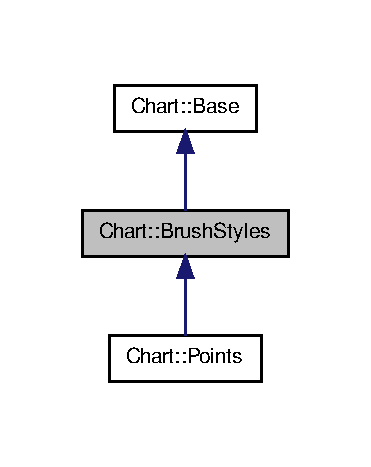
\includegraphics[width=178pt]{classChart_1_1BrushStyles__inherit__graph}
\end{center}
\end{figure}


Collaboration diagram for Chart::BrushStyles:\nopagebreak
\begin{figure}[H]
\begin{center}
\leavevmode
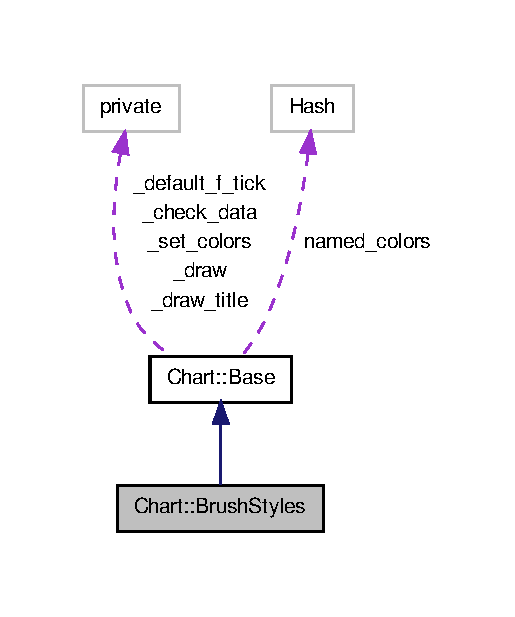
\includegraphics[width=247pt]{classChart_1_1BrushStyles__coll__graph}
\end{center}
\end{figure}
\subsection*{Public Functions}
\label{_amgrpda6bc86800313ecde6e56bd1b41a7c55}
 \begin{DoxyCompactItemize}
\item 
\hyperlink{classChart_1_1BrushStyles_adbd59ea91ba902a765fce4297a69b151}{OpenCircle}
\begin{DoxyCompactList}\small\item\em Set the gdBrush object to have nice brushed object representing a circle of the size \$radius. \item\end{DoxyCompactList}\item 
\hyperlink{classChart_1_1BrushStyles_af84643e28b62d5ddefaf36db4632824a}{FilledCircle}
\begin{DoxyCompactList}\small\item\em Set the gdBrush object to have nice brushed object representing a point of the size \$radius. \item\end{DoxyCompactList}\item 
\hyperlink{classChart_1_1BrushStyles_ae2f9c23e20ca5e9b329d5fe3630fc790}{Star}
\begin{DoxyCompactList}\small\item\em Set the gdBrush object to have nice brushed object representing a star of the size \$radius. \item\end{DoxyCompactList}\item 
\hyperlink{classChart_1_1BrushStyles_a2c807213b768f1a0941cbd7aebee7642}{FilledDiamond}
\begin{DoxyCompactList}\small\item\em Set the gdBrush object to have nice brushed object representing a filled diamond of the size \$radius. \item\end{DoxyCompactList}\item 
\hyperlink{classChart_1_1BrushStyles_affdd85acc56b6be6068c5cc960f9857c}{OpenDiamond}
\begin{DoxyCompactList}\small\item\em Set the gdBrush object to have nice brushed object representing a diamond of the size \$radius-\/1. \item\end{DoxyCompactList}\item 
\hyperlink{classChart_1_1BrushStyles_a3d17237567c35f8844e29e2bc7b03609}{OpenRectangle}
\begin{DoxyCompactList}\small\item\em Set the gdBrush object to have nice brushed object representing a rectangle of the height \$radius-\/1 and width of \$radius/2. \item\end{DoxyCompactList}\end{DoxyCompactItemize}


\subsection{Detailed Description}
Define styles for \hyperlink{classChart_1_1Points}{Points} and \hyperlink{classChart_1_1LinesPoints}{LinesPoints} classes. This class provides functions which define different brush styles to extend the previous point as the only design for \hyperlink{Points_8pm}{Points.pm} or \hyperlink{LinesPoints_8pm}{LinesPoints.pm}\par
\par
 The different brush styles are:\par
 \begin{DoxySeeAlso}{See also}
\hyperlink{classChart_1_1BrushStyles_adbd59ea91ba902a765fce4297a69b151}{OpenCircle}\par
 

\hyperlink{classChart_1_1BrushStyles_af84643e28b62d5ddefaf36db4632824a}{FilledCircle}\par
 

\hyperlink{classChart_1_1BrushStyles_ae2f9c23e20ca5e9b329d5fe3630fc790}{Star}\par
 

\hyperlink{classChart_1_1BrushStyles_affdd85acc56b6be6068c5cc960f9857c}{OpenDiamond}\par
 

\hyperlink{classChart_1_1BrushStyles_a2c807213b768f1a0941cbd7aebee7642}{FilledDiamond}\par
 

\hyperlink{classChart_1_1BrushStyles_a3d17237567c35f8844e29e2bc7b03609}{OpenRectangle}\par
 

FilledRectangle\par
 
\end{DoxySeeAlso}


\subsection{Member Data Documentation}
\hypertarget{classChart_1_1BrushStyles_af84643e28b62d5ddefaf36db4632824a}{
\index{Chart::BrushStyles@{Chart::BrushStyles}!FilledCircle@{FilledCircle}}
\index{FilledCircle@{FilledCircle}!Chart::BrushStyles@{Chart::BrushStyles}}
\subsubsection[{FilledCircle}]{\setlength{\rightskip}{0pt plus 5cm}{\bf Chart::BrushStyles::FilledCircle}}}
\label{classChart_1_1BrushStyles_af84643e28b62d5ddefaf36db4632824a}


Set the gdBrush object to have nice brushed object representing a point of the size \$radius. 


\begin{DoxyParams}{Parameters}
\item[\mbox{\tt[in]} {\em $\ast$GD::Image}]\$rbrush Reference to GD::Image \item[\mbox{\tt[in]} {\em int}]\$radius Radius of the point in pixels \item[\mbox{\tt[in]} {\em int}]\$color Color of the filled point \end{DoxyParams}
\begin{DoxyReturn}{Returns}
nothing
\end{DoxyReturn}
Called by\par
 use \hyperlink{classChart_1_1BrushStyles}{Chart::BrushStyles};\par
 @Chart::Points::ISA = qw(Chart::BrushStyles);\par
 \$self-\/$>$FilledCircle($\backslash$\$rbrush,\$radius, \$color);\par
 to plot the GD::Image representing a filled circle as the point \hypertarget{classChart_1_1BrushStyles_a2c807213b768f1a0941cbd7aebee7642}{
\index{Chart::BrushStyles@{Chart::BrushStyles}!FilledDiamond@{FilledDiamond}}
\index{FilledDiamond@{FilledDiamond}!Chart::BrushStyles@{Chart::BrushStyles}}
\subsubsection[{FilledDiamond}]{\setlength{\rightskip}{0pt plus 5cm}{\bf Chart::BrushStyles::FilledDiamond}}}
\label{classChart_1_1BrushStyles_a2c807213b768f1a0941cbd7aebee7642}


Set the gdBrush object to have nice brushed object representing a filled diamond of the size \$radius. 


\begin{DoxyParams}{Parameters}
\item[\mbox{\tt[in]} {\em $\ast$GD::Image}]\$rbrush Reference to GD::Image \item[\mbox{\tt[in]} {\em int}]\$radius Radius of the diamond in pixels \item[\mbox{\tt[in]} {\em int}]\$color Color of the filled diamond \end{DoxyParams}
\begin{DoxyReturn}{Returns}
nothing
\end{DoxyReturn}
Called by\par
 use \hyperlink{classChart_1_1BrushStyles}{Chart::BrushStyles};\par
 @Chart::Points::ISA = qw(Chart::BrushStyles);\par
 \$self-\/$>$FilledDiamond($\backslash$\$rbrush,\$radius, \$color);\par
 to get back an GD::Image representing a filled diamond as the point \hypertarget{classChart_1_1BrushStyles_adbd59ea91ba902a765fce4297a69b151}{
\index{Chart::BrushStyles@{Chart::BrushStyles}!OpenCircle@{OpenCircle}}
\index{OpenCircle@{OpenCircle}!Chart::BrushStyles@{Chart::BrushStyles}}
\subsubsection[{OpenCircle}]{\setlength{\rightskip}{0pt plus 5cm}{\bf Chart::BrushStyles::OpenCircle}}}
\label{classChart_1_1BrushStyles_adbd59ea91ba902a765fce4297a69b151}


Set the gdBrush object to have nice brushed object representing a circle of the size \$radius. 


\begin{DoxyParams}{Parameters}
\item[\mbox{\tt[in]} {\em $\ast$GD::Image}]\$rbrush Reference to GD::Image \item[\mbox{\tt[in]} {\em int}]\$radius Radius of the point in pixels \item[\mbox{\tt[in]} {\em int}]\$color Color of the not filled point\end{DoxyParams}
Called by\par
 use \hyperlink{classChart_1_1BrushStyles}{Chart::BrushStyles};\par
 @Chart::Points::ISA = qw(Chart::BrushStyles);\par
 \$self-\/$>$OpenCircle($\backslash$\$rbrush,\$radius, \$newcolor);\par
 to plot the GD::Image representing an open circle as the point \hypertarget{classChart_1_1BrushStyles_affdd85acc56b6be6068c5cc960f9857c}{
\index{Chart::BrushStyles@{Chart::BrushStyles}!OpenDiamond@{OpenDiamond}}
\index{OpenDiamond@{OpenDiamond}!Chart::BrushStyles@{Chart::BrushStyles}}
\subsubsection[{OpenDiamond}]{\setlength{\rightskip}{0pt plus 5cm}{\bf Chart::BrushStyles::OpenDiamond}}}
\label{classChart_1_1BrushStyles_affdd85acc56b6be6068c5cc960f9857c}


Set the gdBrush object to have nice brushed object representing a diamond of the size \$radius-\/1. 


\begin{DoxyParams}{Parameters}
\item[\mbox{\tt[in]} {\em $\ast$GD::Image}]\$rbrush Reference to GD::Image \item[\mbox{\tt[in]} {\em int}]\$radius Radius of the diamond in pixels \item[\mbox{\tt[in]} {\em int}]\$color Color of the diamond \end{DoxyParams}
\begin{DoxyReturn}{Returns}
nothing
\end{DoxyReturn}
Called by\par
 use \hyperlink{classChart_1_1BrushStyles}{Chart::BrushStyles};\par
 @Chart::Points::ISA = qw(Chart::BrushStyles);\par
 \$self-\/$>$OpenDiamond($\backslash$\$rbrush,\$radius, \$color);\par
 to get back an GD::Image representing a diamond as the point \hypertarget{classChart_1_1BrushStyles_a3d17237567c35f8844e29e2bc7b03609}{
\index{Chart::BrushStyles@{Chart::BrushStyles}!OpenRectangle@{OpenRectangle}}
\index{OpenRectangle@{OpenRectangle}!Chart::BrushStyles@{Chart::BrushStyles}}
\subsubsection[{OpenRectangle}]{\setlength{\rightskip}{0pt plus 5cm}{\bf Chart::BrushStyles::OpenRectangle}}}
\label{classChart_1_1BrushStyles_a3d17237567c35f8844e29e2bc7b03609}


Set the gdBrush object to have nice brushed object representing a rectangle of the height \$radius-\/1 and width of \$radius/2. 


\begin{DoxyParams}{Parameters}
\item[\mbox{\tt[in]} {\em $\ast$GD::Image}]\$rbrush Reference to GD::Image \item[\mbox{\tt[in]} {\em int}]\$radius Radius of the rectangle in pixels \item[\mbox{\tt[in]} {\em int}]\$color Color of the rectangle \end{DoxyParams}
\begin{DoxyReturn}{Returns}
nothing
\end{DoxyReturn}
Called by\par
 use \hyperlink{classChart_1_1BrushStyles}{Chart::BrushStyles};\par
 @Chart::Points::ISA = qw(Chart::BrushStyles);\par
 \$self-\/$>$OpenDiamond($\backslash$\$rbrush,\$radius, \$color);\par
 to get back an GD::Image representing a rectangle as the point \hypertarget{classChart_1_1BrushStyles_ae2f9c23e20ca5e9b329d5fe3630fc790}{
\index{Chart::BrushStyles@{Chart::BrushStyles}!Star@{Star}}
\index{Star@{Star}!Chart::BrushStyles@{Chart::BrushStyles}}
\subsubsection[{Star}]{\setlength{\rightskip}{0pt plus 5cm}{\bf Chart::BrushStyles::Star}}}
\label{classChart_1_1BrushStyles_ae2f9c23e20ca5e9b329d5fe3630fc790}


Set the gdBrush object to have nice brushed object representing a star of the size \$radius. 


\begin{DoxyParams}{Parameters}
\item[\mbox{\tt[in]} {\em $\ast$GD::Image}]\$rbrush Reference to GD::Image \item[\mbox{\tt[in]} {\em int}]\$radius Radius of the star in pixels \item[\mbox{\tt[in]} {\em int}]\$color Color of the star \end{DoxyParams}
\begin{DoxyReturn}{Returns}
nothing
\end{DoxyReturn}
Called by\par
 use \hyperlink{classChart_1_1BrushStyles}{Chart::BrushStyles};\par
 @Chart::Points::ISA = qw(Chart::BrushStyles);\par
 \$self-\/$>$Star($\backslash$\$rbrush,\$radius, \$color);\par
 to get back an GD::Image representing a star as the point 

The documentation for this class was generated from the following file:\begin{DoxyCompactItemize}
\item 
Chart/\hyperlink{BrushStyles_8pm}{BrushStyles.pm}\end{DoxyCompactItemize}

\hypertarget{classChart_1_1Composite}{
\section{Chart::Composite Class Reference}
\label{classChart_1_1Composite}\index{Chart::Composite@{Chart::Composite}}
}


\hyperlink{classChart_1_1Composite}{Composite} class derived from class \hyperlink{classChart_1_1Base}{Base}.  




Inheritance diagram for Chart::Composite:\nopagebreak
\begin{figure}[H]
\begin{center}
\leavevmode
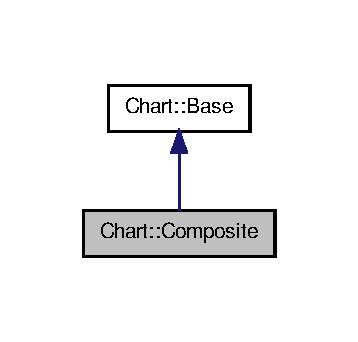
\includegraphics[width=172pt]{classChart_1_1Composite__inherit__graph}
\end{center}
\end{figure}


Collaboration diagram for Chart::Composite:\nopagebreak
\begin{figure}[H]
\begin{center}
\leavevmode
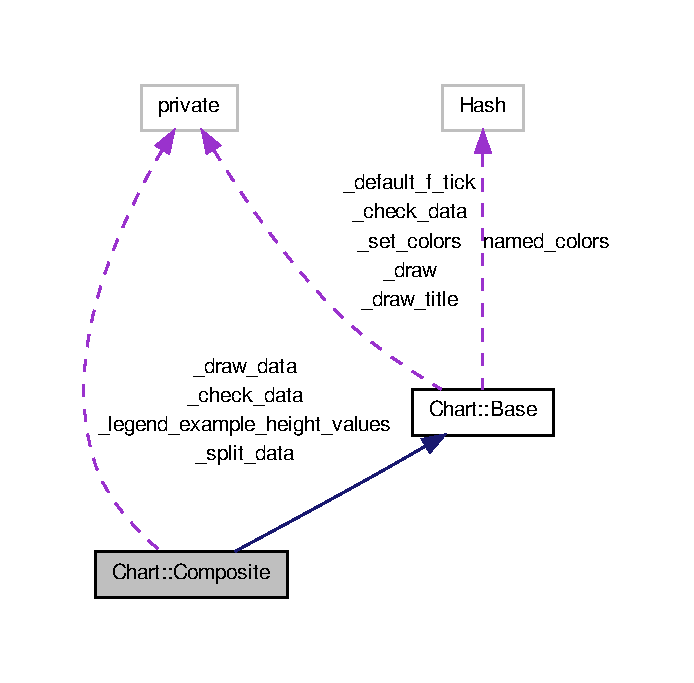
\includegraphics[width=333pt]{classChart_1_1Composite__coll__graph}
\end{center}
\end{figure}
\subsection*{Private Functions}
\label{_amgrp8d29cff216bafa3117e21883ea7c6b5f}
 \begin{DoxyCompactItemize}
\item 
private int \hyperlink{classChart_1_1Composite_a67af0ad77d0c1f4f74da434ceb9cf53c}{\_\-check\_\-data}
\begin{DoxyCompactList}\small\item\em Overwrite \_\-check\_\-data of \hyperlink{classChart_1_1Base}{Chart::Base} and check the internal data to be displayed. \item\end{DoxyCompactList}\item 
private \hyperlink{classChart_1_1Composite_ae4eb768b4ef9d49dc0011bc3f49dab93}{\_\-split\_\-data}
\begin{DoxyCompactList}\small\item\em split data to the composited classes \item\end{DoxyCompactList}\item 
\hypertarget{classChart_1_1Composite_a9fdfe5ec7b8e6aa63797d1e9ae0e4536}{
private \hyperlink{classChart_1_1Composite_a9fdfe5ec7b8e6aa63797d1e9ae0e4536}{\_\-draw\_\-data}}
\label{classChart_1_1Composite_a9fdfe5ec7b8e6aa63797d1e9ae0e4536}

\begin{DoxyCompactList}\small\item\em finally get around to plotting the data for composite chart \item\end{DoxyCompactList}\item 
private \hyperlink{classChart_1_1Composite_aa088e48fc82810b46bde41f468897335}{\_\-legend\_\-example\_\-height\_\-values}
\begin{DoxyCompactList}\small\item\em init the legend\_\-example\_\-height\_\-values \item\end{DoxyCompactList}\item 
private int \hyperlink{classChart_1_1Composite_afcfacbb3cf9fde5a3d9debd6daca3291}{\_\-draw\_\-legend} ()
\begin{DoxyCompactList}\small\item\em let the user know what all the pretty colors mean \item\end{DoxyCompactList}\item 
private int \hyperlink{classChart_1_1Composite_a844a6a68ef755e13236e013decf9cddf}{\_\-draw\_\-top\_\-legend} ()
\begin{DoxyCompactList}\small\item\em put the legend on the top of the data plot \item\end{DoxyCompactList}\item 
private int \hyperlink{classChart_1_1Composite_ae2376bb07ec85374f24b76ac0dbc813a}{\_\-draw\_\-right\_\-legend} ()
\begin{DoxyCompactList}\small\item\em put the legend on the right of the chart \item\end{DoxyCompactList}\item 
private int \hyperlink{classChart_1_1Composite_aaf2a13312cf3fda279eb6b7e37188027}{\_\-draw\_\-left\_\-legend} ()
\begin{DoxyCompactList}\small\item\em draw the legend at the left of the data plot \item\end{DoxyCompactList}\item 
private int \hyperlink{classChart_1_1Composite_a91f9c46886e61ae81057a7489632f366}{\_\-draw\_\-bottom\_\-legend} ()
\begin{DoxyCompactList}\small\item\em put the legend on the bottom of the chart \item\end{DoxyCompactList}\item 
private int \hyperlink{classChart_1_1Composite_a1f58fe4c7a6db069a7f4e173ac76a961}{\_\-draw\_\-none\_\-legend} ()
\begin{DoxyCompactList}\small\item\em no legend to draw. \item\end{DoxyCompactList}\item 
private int \hyperlink{classChart_1_1Composite_a7851868c22518f010a467689cec79b93}{\_\-draw\_\-ticks} ()
\begin{DoxyCompactList}\small\item\em draw the ticks and tick labels \item\end{DoxyCompactList}\item 
private int \hyperlink{classChart_1_1Composite_a346409df6cbd56dae5206294a8e9edcb}{\_\-draw\_\-x\_\-ticks} ()
\begin{DoxyCompactList}\small\item\em draw the x-\/ticks and their labels \item\end{DoxyCompactList}\item 
private int \hyperlink{classChart_1_1Composite_a62fd62f54c05506571d4603e5618af30}{\_\-draw\_\-y\_\-ticks} ()
\begin{DoxyCompactList}\small\item\em draw the y-\/ticks and their labels \item\end{DoxyCompactList}\item 
private \hyperlink{classChart_1_1Composite_ac06ff37b9ca2891fa2a11ce3368a7f6e}{\_\-sub\_\-update} ()
\begin{DoxyCompactList}\small\item\em update all the necessary information in the sub-\/objects \item\end{DoxyCompactList}\item 
private \hyperlink{classChart_1_1Composite_a0db68b32279d7b19c3a0336a24bc360c}{\_\-boundary\_\-update} ()
\begin{DoxyCompactList}\small\item\em copy the current gd\_\-obj boundaries from one object to another \item\end{DoxyCompactList}\item 
private int \hyperlink{classChart_1_1Composite_a6a727845be209cb4d9cb825ab6c5ffb1}{\_\-draw\_\-y\_\-grid\_\-lines} ()
\begin{DoxyCompactList}\small\item\em draw grid\_\-lines for y \item\end{DoxyCompactList}\item 
private int \hyperlink{classChart_1_1Composite_a37406d5ce28e2e8a0465eeff8bfd6911}{\_\-draw\_\-y2\_\-grid\_\-lines} ()
\begin{DoxyCompactList}\small\item\em draw grid\_\-lines for y \item\end{DoxyCompactList}\end{DoxyCompactItemize}
\subsection*{Public Object Methods}
\label{_amgrpfb74d91261823cc595bbeff1eff2b9d5}
 \begin{DoxyCompactItemize}
\item 
int \hyperlink{classChart_1_1Composite_a00e87797c96ce57efc6b066cbe7d6333}{set} (hash opts)
\begin{DoxyCompactList}\small\item\em Set all options. \item\end{DoxyCompactList}\end{DoxyCompactItemize}
\subsection*{Public Functions}
\label{_amgrpda6bc86800313ecde6e56bd1b41a7c55}
 \begin{DoxyCompactItemize}
\item 
\hyperlink{classChart_1_1Composite_ab8dbbeec3544f8e9b1b10486aa46459d}{imagemap\_\-dump} ()
\begin{DoxyCompactList}\small\item\em Overwrite function imagemap\_\-dump of base class. \item\end{DoxyCompactList}\end{DoxyCompactItemize}
\subsection*{Protected Functions}
\label{_amgrp1be0c318101080497e412caf5a02ec65}
 \begin{DoxyCompactItemize}
\item 
\hypertarget{classChart_1_1Composite_ada84d557f9ee7ba91de68103b092ec05}{
protected retval {\bfseries \_\-\_\-print\_\-array} ()}
\label{classChart_1_1Composite_ada84d557f9ee7ba91de68103b092ec05}

\end{DoxyCompactItemize}


\subsection{Detailed Description}
\hyperlink{classChart_1_1Composite}{Composite} class derived from class \hyperlink{classChart_1_1Base}{Base}. \par
 This class provides all functions which are specific to composite charts 

\subsection{Member Function Documentation}
\hypertarget{classChart_1_1Composite_a0db68b32279d7b19c3a0336a24bc360c}{
\index{Chart::Composite@{Chart::Composite}!\_\-boundary\_\-update@{\_\-boundary\_\-update}}
\index{\_\-boundary\_\-update@{\_\-boundary\_\-update}!Chart::Composite@{Chart::Composite}}
\subsubsection[{\_\-boundary\_\-update}]{\setlength{\rightskip}{0pt plus 5cm}private Chart::Composite::\_\-boundary\_\-update (
\begin{DoxyParamCaption}
{}
\end{DoxyParamCaption}
)}}
\label{classChart_1_1Composite_a0db68b32279d7b19c3a0336a24bc360c}


copy the current gd\_\-obj boundaries from one object to another 

Only for \hyperlink{classChart_1_1Composite}{Chart::Composite} \hypertarget{classChart_1_1Composite_a91f9c46886e61ae81057a7489632f366}{
\index{Chart::Composite@{Chart::Composite}!\_\-draw\_\-bottom\_\-legend@{\_\-draw\_\-bottom\_\-legend}}
\index{\_\-draw\_\-bottom\_\-legend@{\_\-draw\_\-bottom\_\-legend}!Chart::Composite@{Chart::Composite}}
\subsubsection[{\_\-draw\_\-bottom\_\-legend}]{\setlength{\rightskip}{0pt plus 5cm}private int Chart::Composite::\_\-draw\_\-bottom\_\-legend (
\begin{DoxyParamCaption}
{}
\end{DoxyParamCaption}
)}}
\label{classChart_1_1Composite_a91f9c46886e61ae81057a7489632f366}


put the legend on the bottom of the chart 

Overwrite the base class \_\-draw\_\-bottom\_\-legend

\begin{DoxyReturn}{Returns}
status 
\end{DoxyReturn}


Reimplemented from \hyperlink{classChart_1_1Base_a863d96ec45b7fbd5ff05194f4eb827d0}{Chart::Base}.

\hypertarget{classChart_1_1Composite_aaf2a13312cf3fda279eb6b7e37188027}{
\index{Chart::Composite@{Chart::Composite}!\_\-draw\_\-left\_\-legend@{\_\-draw\_\-left\_\-legend}}
\index{\_\-draw\_\-left\_\-legend@{\_\-draw\_\-left\_\-legend}!Chart::Composite@{Chart::Composite}}
\subsubsection[{\_\-draw\_\-left\_\-legend}]{\setlength{\rightskip}{0pt plus 5cm}private int Chart::Composite::\_\-draw\_\-left\_\-legend (
\begin{DoxyParamCaption}
{}
\end{DoxyParamCaption}
)}}
\label{classChart_1_1Composite_aaf2a13312cf3fda279eb6b7e37188027}


draw the legend at the left of the data plot 

Overwrite the base class \_\-draw\_\-left\_\-legend

\begin{DoxyReturn}{Returns}
status 
\end{DoxyReturn}


Reimplemented from \hyperlink{classChart_1_1Base_a39bad67aecd83bf523bc27d397256480}{Chart::Base}.

\hypertarget{classChart_1_1Composite_afcfacbb3cf9fde5a3d9debd6daca3291}{
\index{Chart::Composite@{Chart::Composite}!\_\-draw\_\-legend@{\_\-draw\_\-legend}}
\index{\_\-draw\_\-legend@{\_\-draw\_\-legend}!Chart::Composite@{Chart::Composite}}
\subsubsection[{\_\-draw\_\-legend}]{\setlength{\rightskip}{0pt plus 5cm}private int Chart::Composite::\_\-draw\_\-legend (
\begin{DoxyParamCaption}
{}
\end{DoxyParamCaption}
)}}
\label{classChart_1_1Composite_afcfacbb3cf9fde5a3d9debd6daca3291}


let the user know what all the pretty colors mean 

\begin{DoxyReturn}{Returns}
status 
\end{DoxyReturn}


Reimplemented from \hyperlink{classChart_1_1Base_a530e742ca18ce2e89f177d367964277f}{Chart::Base}.

\hypertarget{classChart_1_1Composite_a1f58fe4c7a6db069a7f4e173ac76a961}{
\index{Chart::Composite@{Chart::Composite}!\_\-draw\_\-none\_\-legend@{\_\-draw\_\-none\_\-legend}}
\index{\_\-draw\_\-none\_\-legend@{\_\-draw\_\-none\_\-legend}!Chart::Composite@{Chart::Composite}}
\subsubsection[{\_\-draw\_\-none\_\-legend}]{\setlength{\rightskip}{0pt plus 5cm}private int Chart::Composite::\_\-draw\_\-none\_\-legend (
\begin{DoxyParamCaption}
{}
\end{DoxyParamCaption}
)}}
\label{classChart_1_1Composite_a1f58fe4c7a6db069a7f4e173ac76a961}


no legend to draw. 

. just update the color tables for subs

This routine overwrites this function of the \hyperlink{classChart_1_1Base}{Base} class

\begin{DoxyReturn}{Returns}
status 
\end{DoxyReturn}


Reimplemented from \hyperlink{classChart_1_1Base_a2ec9e89bd6719e178877577a72750cb7}{Chart::Base}.

\hypertarget{classChart_1_1Composite_ae2376bb07ec85374f24b76ac0dbc813a}{
\index{Chart::Composite@{Chart::Composite}!\_\-draw\_\-right\_\-legend@{\_\-draw\_\-right\_\-legend}}
\index{\_\-draw\_\-right\_\-legend@{\_\-draw\_\-right\_\-legend}!Chart::Composite@{Chart::Composite}}
\subsubsection[{\_\-draw\_\-right\_\-legend}]{\setlength{\rightskip}{0pt plus 5cm}private int Chart::Composite::\_\-draw\_\-right\_\-legend (
\begin{DoxyParamCaption}
{}
\end{DoxyParamCaption}
)}}
\label{classChart_1_1Composite_ae2376bb07ec85374f24b76ac0dbc813a}


put the legend on the right of the chart 

Overwrite the base class \_\-draw\_\-right\_\-legend

\begin{DoxyReturn}{Returns}
status 
\end{DoxyReturn}


Reimplemented from \hyperlink{classChart_1_1Base_a39f25b556f2d82e176fc6b0ccfc6da17}{Chart::Base}.

\hypertarget{classChart_1_1Composite_a7851868c22518f010a467689cec79b93}{
\index{Chart::Composite@{Chart::Composite}!\_\-draw\_\-ticks@{\_\-draw\_\-ticks}}
\index{\_\-draw\_\-ticks@{\_\-draw\_\-ticks}!Chart::Composite@{Chart::Composite}}
\subsubsection[{\_\-draw\_\-ticks}]{\setlength{\rightskip}{0pt plus 5cm}private int Chart::Composite::\_\-draw\_\-ticks (
\begin{DoxyParamCaption}
{}
\end{DoxyParamCaption}
)}}
\label{classChart_1_1Composite_a7851868c22518f010a467689cec79b93}


draw the ticks and tick labels 

Overwrites function \hyperlink{classChart_1_1Composite_a7851868c22518f010a467689cec79b93}{\_\-draw\_\-ticks()} of base class

\begin{DoxyReturn}{Returns}
status 
\end{DoxyReturn}


Reimplemented from \hyperlink{classChart_1_1Base_a26f0a0f81ae5e6082c2e7f7c00981dac}{Chart::Base}.

\hypertarget{classChart_1_1Composite_a844a6a68ef755e13236e013decf9cddf}{
\index{Chart::Composite@{Chart::Composite}!\_\-draw\_\-top\_\-legend@{\_\-draw\_\-top\_\-legend}}
\index{\_\-draw\_\-top\_\-legend@{\_\-draw\_\-top\_\-legend}!Chart::Composite@{Chart::Composite}}
\subsubsection[{\_\-draw\_\-top\_\-legend}]{\setlength{\rightskip}{0pt plus 5cm}private int Chart::Composite::\_\-draw\_\-top\_\-legend (
\begin{DoxyParamCaption}
{}
\end{DoxyParamCaption}
)}}
\label{classChart_1_1Composite_a844a6a68ef755e13236e013decf9cddf}


put the legend on the top of the data plot 

Overwrite the base class \_\-draw\_\-top\_\-legend

\begin{DoxyReturn}{Returns}
status 
\end{DoxyReturn}


Reimplemented from \hyperlink{classChart_1_1Base_a2f3f15efadc46484126c94780748a534}{Chart::Base}.

\hypertarget{classChart_1_1Composite_a346409df6cbd56dae5206294a8e9edcb}{
\index{Chart::Composite@{Chart::Composite}!\_\-draw\_\-x\_\-ticks@{\_\-draw\_\-x\_\-ticks}}
\index{\_\-draw\_\-x\_\-ticks@{\_\-draw\_\-x\_\-ticks}!Chart::Composite@{Chart::Composite}}
\subsubsection[{\_\-draw\_\-x\_\-ticks}]{\setlength{\rightskip}{0pt plus 5cm}private int Chart::Composite::\_\-draw\_\-x\_\-ticks (
\begin{DoxyParamCaption}
{}
\end{DoxyParamCaption}
)}}
\label{classChart_1_1Composite_a346409df6cbd56dae5206294a8e9edcb}


draw the x-\/ticks and their labels 

Overwrites function \hyperlink{classChart_1_1Composite_a346409df6cbd56dae5206294a8e9edcb}{\_\-draw\_\-x\_\-ticks()} of base class

\begin{DoxyReturn}{Returns}
status 
\end{DoxyReturn}


Reimplemented from \hyperlink{classChart_1_1Base_a64a81b266a528e24e5547ac504c1fc78}{Chart::Base}.

\hypertarget{classChart_1_1Composite_a37406d5ce28e2e8a0465eeff8bfd6911}{
\index{Chart::Composite@{Chart::Composite}!\_\-draw\_\-y2\_\-grid\_\-lines@{\_\-draw\_\-y2\_\-grid\_\-lines}}
\index{\_\-draw\_\-y2\_\-grid\_\-lines@{\_\-draw\_\-y2\_\-grid\_\-lines}!Chart::Composite@{Chart::Composite}}
\subsubsection[{\_\-draw\_\-y2\_\-grid\_\-lines}]{\setlength{\rightskip}{0pt plus 5cm}private int Chart::Composite::\_\-draw\_\-y2\_\-grid\_\-lines (
\begin{DoxyParamCaption}
{}
\end{DoxyParamCaption}
)}}
\label{classChart_1_1Composite_a37406d5ce28e2e8a0465eeff8bfd6911}


draw grid\_\-lines for y 

Overwrites this function of \hyperlink{classChart_1_1Base}{Base} 

Reimplemented from \hyperlink{classChart_1_1Base_af174cccca9ebbc23f588b6587e88fa1b}{Chart::Base}.

\hypertarget{classChart_1_1Composite_a6a727845be209cb4d9cb825ab6c5ffb1}{
\index{Chart::Composite@{Chart::Composite}!\_\-draw\_\-y\_\-grid\_\-lines@{\_\-draw\_\-y\_\-grid\_\-lines}}
\index{\_\-draw\_\-y\_\-grid\_\-lines@{\_\-draw\_\-y\_\-grid\_\-lines}!Chart::Composite@{Chart::Composite}}
\subsubsection[{\_\-draw\_\-y\_\-grid\_\-lines}]{\setlength{\rightskip}{0pt plus 5cm}private int Chart::Composite::\_\-draw\_\-y\_\-grid\_\-lines (
\begin{DoxyParamCaption}
{}
\end{DoxyParamCaption}
)}}
\label{classChart_1_1Composite_a6a727845be209cb4d9cb825ab6c5ffb1}


draw grid\_\-lines for y 

Overwrites this function of \hyperlink{classChart_1_1Base}{Base} 

Reimplemented from \hyperlink{classChart_1_1Base_aac178efe7b3c275cd18fe3c86b4d7a6f}{Chart::Base}.

\hypertarget{classChart_1_1Composite_a62fd62f54c05506571d4603e5618af30}{
\index{Chart::Composite@{Chart::Composite}!\_\-draw\_\-y\_\-ticks@{\_\-draw\_\-y\_\-ticks}}
\index{\_\-draw\_\-y\_\-ticks@{\_\-draw\_\-y\_\-ticks}!Chart::Composite@{Chart::Composite}}
\subsubsection[{\_\-draw\_\-y\_\-ticks}]{\setlength{\rightskip}{0pt plus 5cm}private int Chart::Composite::\_\-draw\_\-y\_\-ticks (
\begin{DoxyParamCaption}
{}
\end{DoxyParamCaption}
)}}
\label{classChart_1_1Composite_a62fd62f54c05506571d4603e5618af30}


draw the y-\/ticks and their labels 

Overwrites function \hyperlink{classChart_1_1Composite_a62fd62f54c05506571d4603e5618af30}{\_\-draw\_\-y\_\-ticks()} of base class

\begin{DoxyReturn}{Returns}
status 
\end{DoxyReturn}


Reimplemented from \hyperlink{classChart_1_1Base_a46852297ab12aaf10546e63dd7eab462}{Chart::Base}.

\hypertarget{classChart_1_1Composite_ac06ff37b9ca2891fa2a11ce3368a7f6e}{
\index{Chart::Composite@{Chart::Composite}!\_\-sub\_\-update@{\_\-sub\_\-update}}
\index{\_\-sub\_\-update@{\_\-sub\_\-update}!Chart::Composite@{Chart::Composite}}
\subsubsection[{\_\-sub\_\-update}]{\setlength{\rightskip}{0pt plus 5cm}private Chart::Composite::\_\-sub\_\-update (
\begin{DoxyParamCaption}
{}
\end{DoxyParamCaption}
)}}
\label{classChart_1_1Composite_ac06ff37b9ca2891fa2a11ce3368a7f6e}


update all the necessary information in the sub-\/objects 

Only for \hyperlink{classChart_1_1Composite}{Chart::Composite} \hypertarget{classChart_1_1Composite_ab8dbbeec3544f8e9b1b10486aa46459d}{
\index{Chart::Composite@{Chart::Composite}!imagemap\_\-dump@{imagemap\_\-dump}}
\index{imagemap\_\-dump@{imagemap\_\-dump}!Chart::Composite@{Chart::Composite}}
\subsubsection[{imagemap\_\-dump}]{\setlength{\rightskip}{0pt plus 5cm}Chart::Composite::imagemap\_\-dump (
\begin{DoxyParamCaption}
{}
\end{DoxyParamCaption}
)}}
\label{classChart_1_1Composite_ab8dbbeec3544f8e9b1b10486aa46459d}


Overwrite function imagemap\_\-dump of base class. 

Get the information to turn the chart into an imagemap had to override it to reassemble the @data array correctly

\begin{DoxyReturn}{Returns}
Reference to an array of the image 
\end{DoxyReturn}


Reimplemented from \hyperlink{classChart_1_1Base_af9fec7910f7254177a81252a03a0f587}{Chart::Base}.

\hypertarget{classChart_1_1Composite_a00e87797c96ce57efc6b066cbe7d6333}{
\index{Chart::Composite@{Chart::Composite}!set@{set}}
\index{set@{set}!Chart::Composite@{Chart::Composite}}
\subsubsection[{set}]{\setlength{\rightskip}{0pt plus 5cm}int Chart::Composite::set (
\begin{DoxyParamCaption}
\item[{hash}]{ opts}
\end{DoxyParamCaption}
)}}
\label{classChart_1_1Composite_a00e87797c96ce57efc6b066cbe7d6333}


Set all options. 


\begin{DoxyParams}{Parameters}
\item[\mbox{\tt[in]} {\em \%opts}]Hash of options to the Chart \end{DoxyParams}
\begin{DoxyReturn}{Returns}
ok or croak
\end{DoxyReturn}
Overwrite the set function of class \hyperlink{classChart_1_1Base}{Base} to pass options to the sub-\/objects later 

Reimplemented from \hyperlink{classChart_1_1Base_aadd99033eae9eab891cc2abdf7e4b74d}{Chart::Base}.



\subsection{Member Data Documentation}
\hypertarget{classChart_1_1Composite_a67af0ad77d0c1f4f74da434ceb9cf53c}{
\index{Chart::Composite@{Chart::Composite}!\_\-check\_\-data@{\_\-check\_\-data}}
\index{\_\-check\_\-data@{\_\-check\_\-data}!Chart::Composite@{Chart::Composite}}
\subsubsection[{\_\-check\_\-data}]{\setlength{\rightskip}{0pt plus 5cm}private int {\bf Chart::Composite::\_\-check\_\-data}}}
\label{classChart_1_1Composite_a67af0ad77d0c1f4f74da434ceb9cf53c}


Overwrite \_\-check\_\-data of \hyperlink{classChart_1_1Base}{Chart::Base} and check the internal data to be displayed. 

Make sure the data isn't really weird and collect some basic info about it\par
 \begin{DoxyReturn}{Returns}
status of check 
\end{DoxyReturn}


Reimplemented from \hyperlink{classChart_1_1Base_a13296be5b92a9880851977fe0abfdf01}{Chart::Base}.

\hypertarget{classChart_1_1Composite_aa088e48fc82810b46bde41f468897335}{
\index{Chart::Composite@{Chart::Composite}!\_\-legend\_\-example\_\-height\_\-values@{\_\-legend\_\-example\_\-height\_\-values}}
\index{\_\-legend\_\-example\_\-height\_\-values@{\_\-legend\_\-example\_\-height\_\-values}!Chart::Composite@{Chart::Composite}}
\subsubsection[{\_\-legend\_\-example\_\-height\_\-values}]{\setlength{\rightskip}{0pt plus 5cm}private {\bf Chart::Composite::\_\-legend\_\-example\_\-height\_\-values}}}
\label{classChart_1_1Composite_aa088e48fc82810b46bde41f468897335}


init the legend\_\-example\_\-height\_\-values 

\hypertarget{classChart_1_1Composite_ae4eb768b4ef9d49dc0011bc3f49dab93}{
\index{Chart::Composite@{Chart::Composite}!\_\-split\_\-data@{\_\-split\_\-data}}
\index{\_\-split\_\-data@{\_\-split\_\-data}!Chart::Composite@{Chart::Composite}}
\subsubsection[{\_\-split\_\-data}]{\setlength{\rightskip}{0pt plus 5cm}private {\bf Chart::Composite::\_\-split\_\-data}}}
\label{classChart_1_1Composite_ae4eb768b4ef9d49dc0011bc3f49dab93}


split data to the composited classes 

create sub-\/objects for each type, store the appropriate data sets in each one, and stick the correct values into them (ie. 'gd\_\-obj'); 

The documentation for this class was generated from the following file:\begin{DoxyCompactItemize}
\item 
Chart/\hyperlink{Composite_8pm}{Composite.pm}\end{DoxyCompactItemize}

\hypertarget{classChart_1_1Constants}{
\section{Chart::Constants Class Reference}
\label{classChart_1_1Constants}\index{Chart::Constants@{Chart::Constants}}
}


\hyperlink{classChart_1_1Constants}{Constants} class defines all necessary constants for Class Chart.  




\subsection{Detailed Description}
\hyperlink{classChart_1_1Constants}{Constants} class defines all necessary constants for Class Chart. Defined are \par
 PI = 3.141...\par
 \par
 Usage:\par
 use Chart:\hyperlink{classChart_1_1Constants}{Constants}; ...\par
 My \$pi = Chart::Constants::PI;\par
 ...\par
 

The documentation for this class was generated from the following file:\begin{DoxyCompactItemize}
\item 
Chart/\hyperlink{Constants_8pm}{Constants.pm}\end{DoxyCompactItemize}

\hypertarget{classChart_1_1Direction}{
\section{Chart::Direction Class Reference}
\label{classChart_1_1Direction}\index{Chart::Direction@{Chart::Direction}}
}


\hyperlink{classChart_1_1Direction}{Direction} class derived class for Chart to implement direction charts.  




Inheritance diagram for Chart::Direction:\nopagebreak
\begin{figure}[H]
\begin{center}
\leavevmode
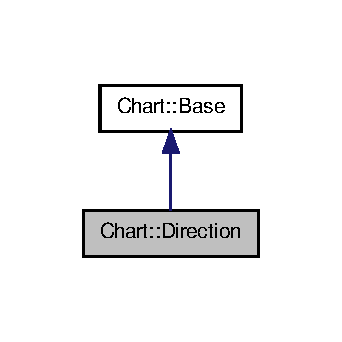
\includegraphics[width=164pt]{classChart_1_1Direction__inherit__graph}
\end{center}
\end{figure}


Collaboration diagram for Chart::Direction:\nopagebreak
\begin{figure}[H]
\begin{center}
\leavevmode
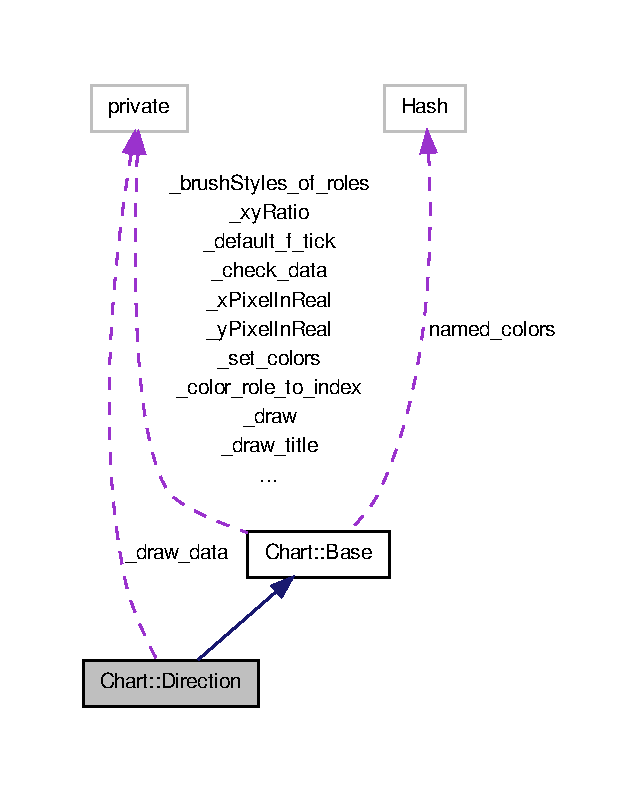
\includegraphics[width=307pt]{classChart_1_1Direction__coll__graph}
\end{center}
\end{figure}
\subsection*{Private Functions}
\label{_amgrp8d29cff216bafa3117e21883ea7c6b5f}
 \begin{DoxyCompactItemize}
\item 
\hypertarget{classChart_1_1Direction_af97c0fecf23820586656d100aed65008}{
private \hyperlink{classChart_1_1Direction_af97c0fecf23820586656d100aed65008}{\_\-draw\_\-data}}
\label{classChart_1_1Direction_af97c0fecf23820586656d100aed65008}

\begin{DoxyCompactList}\small\item\em finally get around to plotting the data for direction charts \item\end{DoxyCompactList}\item 
private int \hyperlink{classChart_1_1Direction_ad33ea739bd5ceb8b48809028c489f119}{\_\-find\_\-y\_\-scale} ()
\begin{DoxyCompactList}\small\item\em we use the find\_\-y\_\-scale methode to determine the labels of the circles and the amount of them \item\end{DoxyCompactList}\item 
private \hyperlink{classChart_1_1Direction_a6766001399b56ba88e61f7ca0db50922}{\_\-calcTickInterval} (scalar dataset\_\-min, scalar dataset\_\-max, scalar flag\_\-fixed\_\-min, scalar flag\_\-fixed\_\-max, scalar minTicks, scalar maxTicks)
\begin{DoxyCompactList}\small\item\em Calculates the ticks for direction in normalised units. \item\end{DoxyCompactList}\item 
private int \hyperlink{classChart_1_1Direction_aae701e9961733ae43e068acbad3e139a}{\_\-draw\_\-y\_\-ticks} ()
\begin{DoxyCompactList}\small\item\em draw the circles and the axes \item\end{DoxyCompactList}\item 
private int \hyperlink{classChart_1_1Direction_a4803bef9580feed235401ff290459cce}{\_\-draw\_\-x\_\-ticks} ()
\begin{DoxyCompactList}\small\item\em We don't need x ticks, it's all done in \_\-draw\_\-y\_\-ticks. \item\end{DoxyCompactList}\item 
private int \hyperlink{classChart_1_1Direction_aa40aa25ffd6c9005303642e1d0ce1ae6}{\_\-prepare\_\-brush} (scalar color, scalar type)
\begin{DoxyCompactList}\small\item\em set the gdBrush object to trick GD into drawing fat lines \item\end{DoxyCompactList}\item 
private int \hyperlink{classChart_1_1Direction_a47ab5b61307d24d038ae77e62e269099}{\_\-draw\_\-legend} ()
\begin{DoxyCompactList}\small\item\em let them know what all the pretty colors mean \item\end{DoxyCompactList}\item 
private array \hyperlink{classChart_1_1Direction_a8f408c9fa61c3ee5f87a19c1f42d94c7}{\_\-find\_\-y\_\-range} ()
\begin{DoxyCompactList}\small\item\em Find minimum and maximum value of y data sets. \item\end{DoxyCompactList}\end{DoxyCompactItemize}
\subsection*{Public Object Methods}
\label{_amgrpfb74d91261823cc595bbeff1eff2b9d5}
\begin{Desc}
\item[\hyperlink{todo__todo000001}{Todo}]calculate the width of the labels \end{Desc}
\begin{DoxyCompactItemize}
\item 
int \hyperlink{classChart_1_1Direction_ab7104b48aa4219a995656088c121078d}{set} (hash opts)
\begin{DoxyCompactList}\small\item\em Set all options. \item\end{DoxyCompactList}\item 
int \hyperlink{classChart_1_1Direction_a50b338ce75f7e6ab339b5f587a4e933b}{add\_\-dataset} (list data)
\begin{DoxyCompactList}\small\item\em Add many datasets to the dataref. \item\end{DoxyCompactList}\end{DoxyCompactItemize}
\subsection*{Protected Object Methods}
\label{_amgrp06e02ce997685862181738d6a83b6f25}
 \begin{DoxyCompactItemize}
\item 
\hypertarget{classChart_1_1Direction_a9e77fdb40ac62f9a18becd46fd1923ce}{
protected retval {\bfseries \_\-calcTickInterval} ()}
\label{classChart_1_1Direction_a9e77fdb40ac62f9a18becd46fd1923ce}

\end{DoxyCompactItemize}


\subsection{Detailed Description}
\hyperlink{classChart_1_1Direction}{Direction} class derived class for Chart to implement direction charts. 

\subsection{Member Function Documentation}
\hypertarget{classChart_1_1Direction_a6766001399b56ba88e61f7ca0db50922}{
\index{Chart::Direction@{Chart::Direction}!\_\-calcTickInterval@{\_\-calcTickInterval}}
\index{\_\-calcTickInterval@{\_\-calcTickInterval}!Chart::Direction@{Chart::Direction}}
\subsubsection[{\_\-calcTickInterval}]{\setlength{\rightskip}{0pt plus 5cm}private Chart::Direction::\_\-calcTickInterval (
\begin{DoxyParamCaption}
\item[{scalar}]{ dataset\_\-min, }
\item[{scalar}]{ dataset\_\-max, }
\item[{scalar}]{ flag\_\-fixed\_\-min, }
\item[{scalar}]{ flag\_\-fixed\_\-max, }
\item[{scalar}]{ minTicks, }
\item[{scalar}]{ maxTicks}
\end{DoxyParamCaption}
)}}
\label{classChart_1_1Direction_a6766001399b56ba88e61f7ca0db50922}


Calculates the ticks for direction in normalised units. 

Calculate the Interval between ticks in y direction and compare the number of ticks to the user given values min\_\-y\_\-ticks, max\_\-y\_\-ticks


\begin{DoxyParams}{Parameters}
\item[\mbox{\tt[in]} {\em \$dataset\_\-min}]Minimal value in y direction \item[\mbox{\tt[in]} {\em \$dataset\_\-max}]Maximal value in y direction \item[\mbox{\tt[in]} {\em \$flag\_\-fixed\_\-min}]Indicator whether the dataset\_\-min value is fixed \item[\mbox{\tt[in]} {\em \$flag\_\-fixed\_\-max}]Indicator whether the dataset\_\-max value is fixed \item[\mbox{\tt[in]} {\em \$minTicks}]Minimal number of ticks wanted \item[\mbox{\tt[in]} {\em \$maxTicks}]Maximal number of ticks wanted \end{DoxyParams}
\begin{DoxyReturn}{Returns}
\$tickInterval, \$tickCount, \$pMin, \$pMax 
\end{DoxyReturn}


Reimplemented from \hyperlink{classChart_1_1Base_a23f7394cb8c7bbe6a5d0e05582e038c9}{Chart::Base}.

\hypertarget{classChart_1_1Direction_a47ab5b61307d24d038ae77e62e269099}{
\index{Chart::Direction@{Chart::Direction}!\_\-draw\_\-legend@{\_\-draw\_\-legend}}
\index{\_\-draw\_\-legend@{\_\-draw\_\-legend}!Chart::Direction@{Chart::Direction}}
\subsubsection[{\_\-draw\_\-legend}]{\setlength{\rightskip}{0pt plus 5cm}private int Chart::Direction::\_\-draw\_\-legend (
\begin{DoxyParamCaption}
{}
\end{DoxyParamCaption}
)}}
\label{classChart_1_1Direction_a47ab5b61307d24d038ae77e62e269099}


let them know what all the pretty colors mean 

\begin{DoxyReturn}{Returns}
status
\end{DoxyReturn}
Overwrite corresponding function of \hyperlink{classChart_1_1Base}{Base} 

Reimplemented from \hyperlink{classChart_1_1Base_a530e742ca18ce2e89f177d367964277f}{Chart::Base}.

\hypertarget{classChart_1_1Direction_a4803bef9580feed235401ff290459cce}{
\index{Chart::Direction@{Chart::Direction}!\_\-draw\_\-x\_\-ticks@{\_\-draw\_\-x\_\-ticks}}
\index{\_\-draw\_\-x\_\-ticks@{\_\-draw\_\-x\_\-ticks}!Chart::Direction@{Chart::Direction}}
\subsubsection[{\_\-draw\_\-x\_\-ticks}]{\setlength{\rightskip}{0pt plus 5cm}private int Chart::Direction::\_\-draw\_\-x\_\-ticks (
\begin{DoxyParamCaption}
{}
\end{DoxyParamCaption}
)}}
\label{classChart_1_1Direction_a4803bef9580feed235401ff290459cce}


We don't need x ticks, it's all done in \_\-draw\_\-y\_\-ticks. 

\begin{DoxyReturn}{Returns}
status
\end{DoxyReturn}
Overwrites the corresponding function in \hyperlink{classChart_1_1Base}{Base} 

Reimplemented from \hyperlink{classChart_1_1Base_a64a81b266a528e24e5547ac504c1fc78}{Chart::Base}.

\hypertarget{classChart_1_1Direction_aae701e9961733ae43e068acbad3e139a}{
\index{Chart::Direction@{Chart::Direction}!\_\-draw\_\-y\_\-ticks@{\_\-draw\_\-y\_\-ticks}}
\index{\_\-draw\_\-y\_\-ticks@{\_\-draw\_\-y\_\-ticks}!Chart::Direction@{Chart::Direction}}
\subsubsection[{\_\-draw\_\-y\_\-ticks}]{\setlength{\rightskip}{0pt plus 5cm}private int Chart::Direction::\_\-draw\_\-y\_\-ticks (
\begin{DoxyParamCaption}
{}
\end{DoxyParamCaption}
)}}
\label{classChart_1_1Direction_aae701e9961733ae43e068acbad3e139a}


draw the circles and the axes 

Overwrites \hyperlink{classChart_1_1Direction_aae701e9961733ae43e068acbad3e139a}{\_\-draw\_\-y\_\-ticks()} of \hyperlink{classChart_1_1Base}{Base} class

\begin{DoxyReturn}{Returns}
status 
\end{DoxyReturn}


Reimplemented from \hyperlink{classChart_1_1Base_a46852297ab12aaf10546e63dd7eab462}{Chart::Base}.

\hypertarget{classChart_1_1Direction_a8f408c9fa61c3ee5f87a19c1f42d94c7}{
\index{Chart::Direction@{Chart::Direction}!\_\-find\_\-y\_\-range@{\_\-find\_\-y\_\-range}}
\index{\_\-find\_\-y\_\-range@{\_\-find\_\-y\_\-range}!Chart::Direction@{Chart::Direction}}
\subsubsection[{\_\-find\_\-y\_\-range}]{\setlength{\rightskip}{0pt plus 5cm}private array Chart::Direction::\_\-find\_\-y\_\-range (
\begin{DoxyParamCaption}
{}
\end{DoxyParamCaption}
)}}
\label{classChart_1_1Direction_a8f408c9fa61c3ee5f87a19c1f42d94c7}


Find minimum and maximum value of y data sets. 

\begin{DoxyReturn}{Returns}
( min, max, flag\_\-all\_\-integers )
\end{DoxyReturn}
Overwrites corresponding \hyperlink{classChart_1_1Base}{Base} function 

Reimplemented from \hyperlink{classChart_1_1Base_ad28e18fc86eebc6846785580977532ca}{Chart::Base}.

\hypertarget{classChart_1_1Direction_ad33ea739bd5ceb8b48809028c489f119}{
\index{Chart::Direction@{Chart::Direction}!\_\-find\_\-y\_\-scale@{\_\-find\_\-y\_\-scale}}
\index{\_\-find\_\-y\_\-scale@{\_\-find\_\-y\_\-scale}!Chart::Direction@{Chart::Direction}}
\subsubsection[{\_\-find\_\-y\_\-scale}]{\setlength{\rightskip}{0pt plus 5cm}private int Chart::Direction::\_\-find\_\-y\_\-scale (
\begin{DoxyParamCaption}
{}
\end{DoxyParamCaption}
)}}
\label{classChart_1_1Direction_ad33ea739bd5ceb8b48809028c489f119}


we use the find\_\-y\_\-scale methode to determine the labels of the circles and the amount of them 

\begin{DoxyReturn}{Returns}
status
\end{DoxyReturn}
This function is an overwrite to the same function found in the base class \hyperlink{classChart_1_1Base}{Chart::Base} 

Reimplemented from \hyperlink{classChart_1_1Base_acb2fe91b2d57e43d84b1bc6f092ac68d}{Chart::Base}.

\hypertarget{classChart_1_1Direction_aa40aa25ffd6c9005303642e1d0ce1ae6}{
\index{Chart::Direction@{Chart::Direction}!\_\-prepare\_\-brush@{\_\-prepare\_\-brush}}
\index{\_\-prepare\_\-brush@{\_\-prepare\_\-brush}!Chart::Direction@{Chart::Direction}}
\subsubsection[{\_\-prepare\_\-brush}]{\setlength{\rightskip}{0pt plus 5cm}private int Chart::Direction::\_\-prepare\_\-brush (
\begin{DoxyParamCaption}
\item[{scalar}]{ color, }
\item[{scalar}]{ type}
\end{DoxyParamCaption}
)}}
\label{classChart_1_1Direction_aa40aa25ffd6c9005303642e1d0ce1ae6}


set the gdBrush object to trick GD into drawing fat lines 


\begin{DoxyParams}{Parameters}
\item[{\em \$color}]\item[{\em \$type}]\end{DoxyParams}
\begin{DoxyReturn}{Returns}
status 
\end{DoxyReturn}
\hypertarget{classChart_1_1Direction_a50b338ce75f7e6ab339b5f587a4e933b}{
\index{Chart::Direction@{Chart::Direction}!add\_\-dataset@{add\_\-dataset}}
\index{add\_\-dataset@{add\_\-dataset}!Chart::Direction@{Chart::Direction}}
\subsubsection[{add\_\-dataset}]{\setlength{\rightskip}{0pt plus 5cm}int Chart::Direction::add\_\-dataset (
\begin{DoxyParamCaption}
\item[{list}]{ data}
\end{DoxyParamCaption}
)}}
\label{classChart_1_1Direction_a50b338ce75f7e6ab339b5f587a4e933b}


Add many datasets to the dataref. 

Graph API\par
 Overwrite \hyperlink{classChart_1_1Base}{Base} method


\begin{DoxyParams}{Parameters}
\item[{\em @data}]Dataset to add \end{DoxyParams}


Reimplemented from \hyperlink{classChart_1_1Base_a43dcf87aa2b9fd362ba104923c3f3d51}{Chart::Base}.

\hypertarget{classChart_1_1Direction_ab7104b48aa4219a995656088c121078d}{
\index{Chart::Direction@{Chart::Direction}!set@{set}}
\index{set@{set}!Chart::Direction@{Chart::Direction}}
\subsubsection[{set}]{\setlength{\rightskip}{0pt plus 5cm}int Chart::Direction::set (
\begin{DoxyParamCaption}
\item[{hash}]{ opts}
\end{DoxyParamCaption}
)}}
\label{classChart_1_1Direction_ab7104b48aa4219a995656088c121078d}


Set all options. 


\begin{DoxyParams}{Parameters}
\item[\mbox{\tt[in]} {\em \%opts}]Hash of options to the Chart \end{DoxyParams}
\begin{DoxyReturn}{Returns}
ok or croak
\end{DoxyReturn}
main method for customizing the chart, lets users specify values for different parameters\par
 dont check the number of points in the added datasets in a polarplot\par
 overwrite \hyperlink{classChart_1_1Base}{Base} method 

Reimplemented from \hyperlink{classChart_1_1Base_aadd99033eae9eab891cc2abdf7e4b74d}{Chart::Base}.



The documentation for this class was generated from the following file:\begin{DoxyCompactItemize}
\item 
Chart/\hyperlink{Direction_8pm}{Direction.pm}\end{DoxyCompactItemize}

\hypertarget{classChart_1_1ErrorBars}{
\section{Chart::ErrorBars Class Reference}
\label{classChart_1_1ErrorBars}\index{Chart::ErrorBars@{Chart::ErrorBars}}
}


\hyperlink{classChart_1_1ErrorBars}{ErrorBars} class derived from class \hyperlink{classChart_1_1Base}{Base}.  




Inheritance diagram for Chart::ErrorBars:\nopagebreak
\begin{figure}[H]
\begin{center}
\leavevmode
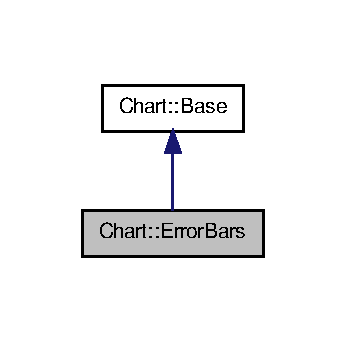
\includegraphics[width=166pt]{classChart_1_1ErrorBars__inherit__graph}
\end{center}
\end{figure}


Collaboration diagram for Chart::ErrorBars:\nopagebreak
\begin{figure}[H]
\begin{center}
\leavevmode
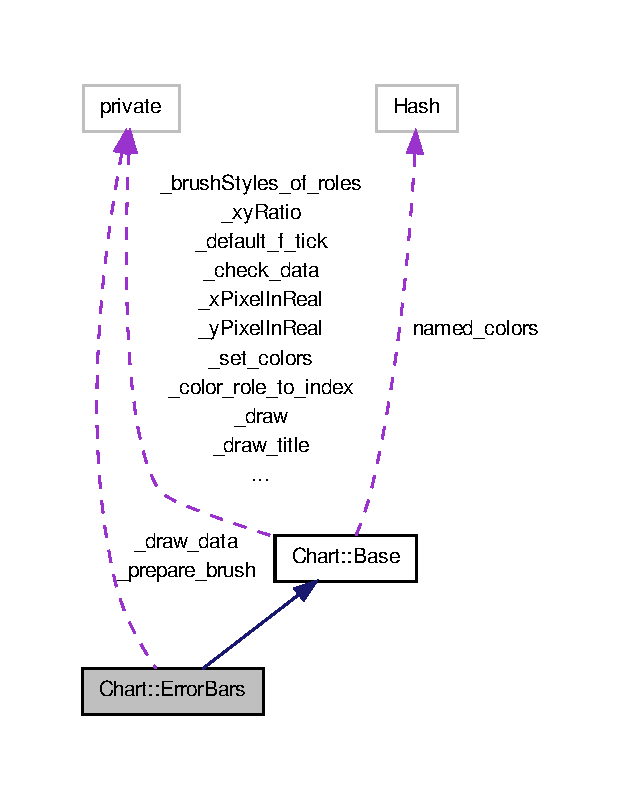
\includegraphics[width=267pt]{classChart_1_1ErrorBars__coll__graph}
\end{center}
\end{figure}
\subsection*{Private Functions}
\label{_amgrp8d29cff216bafa3117e21883ea7c6b5f}
 \begin{DoxyCompactItemize}
\item 
private \hyperlink{classChart_1_1ErrorBars_a33bedf80072c9d80170ff8f3f36813d7}{\_\-draw\_\-data}
\begin{DoxyCompactList}\small\item\em finally get around to plotting the data \item\end{DoxyCompactList}\item 
private \hyperlink{classChart_1_1ErrorBars_aaa3c8ac81fb6af31970112a9780bc825}{\_\-prepare\_\-brush}
\begin{DoxyCompactList}\small\item\em set the gdBrush object to trick GD into drawing fat lines \item\end{DoxyCompactList}\item 
private int \hyperlink{classChart_1_1ErrorBars_a6e1e40b048bbc13bead8449c2b78750a}{\_\-draw\_\-legend} ()
\begin{DoxyCompactList}\small\item\em let them know what all the pretty colors mean \item\end{DoxyCompactList}\end{DoxyCompactItemize}
\subsection*{Protected Object Methods}
\label{_amgrp06e02ce997685862181738d6a83b6f25}
 \begin{DoxyCompactItemize}
\item 
protected retval \hyperlink{classChart_1_1ErrorBars_aa303b7b246e29f54626fecebfe6cf15c}{\_\-find\_\-y\_\-range} ()
\begin{DoxyCompactList}\small\item\em Find minimum and maximum value of y data sets. \item\end{DoxyCompactList}\end{DoxyCompactItemize}


\subsection{Detailed Description}
\hyperlink{classChart_1_1ErrorBars}{ErrorBars} class derived from class \hyperlink{classChart_1_1Base}{Base}. This class provides all functions which are specific to pointes having carrying vertical bars which represent errors or standard deviations 

\subsection{Member Function Documentation}
\hypertarget{classChart_1_1ErrorBars_a6e1e40b048bbc13bead8449c2b78750a}{
\index{Chart::ErrorBars@{Chart::ErrorBars}!\_\-draw\_\-legend@{\_\-draw\_\-legend}}
\index{\_\-draw\_\-legend@{\_\-draw\_\-legend}!Chart::ErrorBars@{Chart::ErrorBars}}
\subsubsection[{\_\-draw\_\-legend}]{\setlength{\rightskip}{0pt plus 5cm}private int Chart::ErrorBars::\_\-draw\_\-legend (
\begin{DoxyParamCaption}
{}
\end{DoxyParamCaption}
)}}
\label{classChart_1_1ErrorBars_a6e1e40b048bbc13bead8449c2b78750a}


let them know what all the pretty colors mean 

\begin{DoxyReturn}{Returns}
status \# let them know what all the pretty colors mean 
\end{DoxyReturn}


Reimplemented from \hyperlink{classChart_1_1Base_a530e742ca18ce2e89f177d367964277f}{Chart::Base}.

\hypertarget{classChart_1_1ErrorBars_aa303b7b246e29f54626fecebfe6cf15c}{
\index{Chart::ErrorBars@{Chart::ErrorBars}!\_\-find\_\-y\_\-range@{\_\-find\_\-y\_\-range}}
\index{\_\-find\_\-y\_\-range@{\_\-find\_\-y\_\-range}!Chart::ErrorBars@{Chart::ErrorBars}}
\subsubsection[{\_\-find\_\-y\_\-range}]{\setlength{\rightskip}{0pt plus 5cm}protected retval Chart::ErrorBars::\_\-find\_\-y\_\-range (
\begin{DoxyParamCaption}
{}
\end{DoxyParamCaption}
)}}
\label{classChart_1_1ErrorBars_aa303b7b246e29f54626fecebfe6cf15c}


Find minimum and maximum value of y data sets. 

\begin{DoxyReturn}{Returns}
( min, max, flag\_\-all\_\-integers ) 
\end{DoxyReturn}


Reimplemented from \hyperlink{classChart_1_1Base_ad28e18fc86eebc6846785580977532ca}{Chart::Base}.



\subsection{Member Data Documentation}
\hypertarget{classChart_1_1ErrorBars_a33bedf80072c9d80170ff8f3f36813d7}{
\index{Chart::ErrorBars@{Chart::ErrorBars}!\_\-draw\_\-data@{\_\-draw\_\-data}}
\index{\_\-draw\_\-data@{\_\-draw\_\-data}!Chart::ErrorBars@{Chart::ErrorBars}}
\subsubsection[{\_\-draw\_\-data}]{\setlength{\rightskip}{0pt plus 5cm}private {\bf Chart::ErrorBars::\_\-draw\_\-data}}}
\label{classChart_1_1ErrorBars_a33bedf80072c9d80170ff8f3f36813d7}


finally get around to plotting the data 

Overwrites \hyperlink{classChart_1_1Base}{Base} function \hypertarget{classChart_1_1ErrorBars_aaa3c8ac81fb6af31970112a9780bc825}{
\index{Chart::ErrorBars@{Chart::ErrorBars}!\_\-prepare\_\-brush@{\_\-prepare\_\-brush}}
\index{\_\-prepare\_\-brush@{\_\-prepare\_\-brush}!Chart::ErrorBars@{Chart::ErrorBars}}
\subsubsection[{\_\-prepare\_\-brush}]{\setlength{\rightskip}{0pt plus 5cm}private {\bf Chart::ErrorBars::\_\-prepare\_\-brush}}}
\label{classChart_1_1ErrorBars_aaa3c8ac81fb6af31970112a9780bc825}


set the gdBrush object to trick GD into drawing fat lines 

Overwrite \hyperlink{classChart_1_1Base}{Base} function 

The documentation for this class was generated from the following file:\begin{DoxyCompactItemize}
\item 
Chart/\hyperlink{ErrorBars_8pm}{ErrorBars.pm}\end{DoxyCompactItemize}

\hypertarget{classChart_1_1HorizontalBars}{
\section{Chart::HorizontalBars Class Reference}
\label{classChart_1_1HorizontalBars}\index{Chart::HorizontalBars@{Chart::HorizontalBars}}
}


\hyperlink{classChart_1_1Bars}{Bars} class derived from class \hyperlink{classChart_1_1Base}{Base}.  




Inheritance diagram for Chart::HorizontalBars:\nopagebreak
\begin{figure}[H]
\begin{center}
\leavevmode
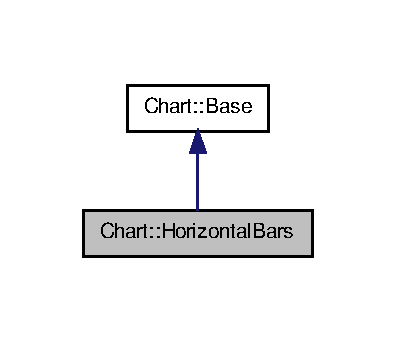
\includegraphics[width=190pt]{classChart_1_1HorizontalBars__inherit__graph}
\end{center}
\end{figure}


Collaboration diagram for Chart::HorizontalBars:\nopagebreak
\begin{figure}[H]
\begin{center}
\leavevmode
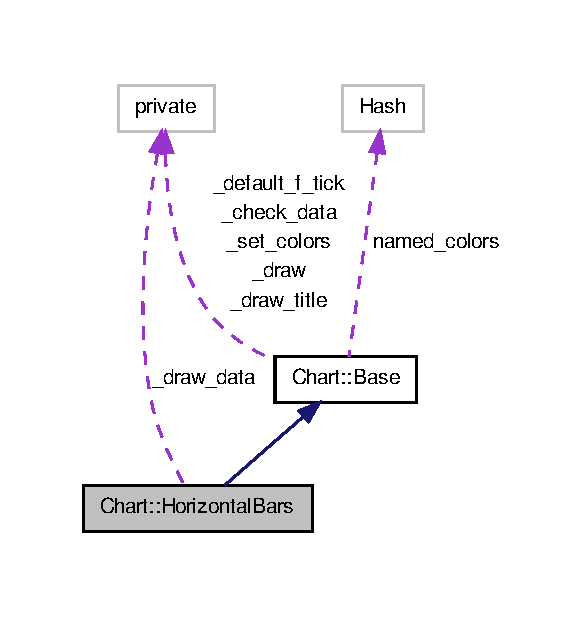
\includegraphics[width=280pt]{classChart_1_1HorizontalBars__coll__graph}
\end{center}
\end{figure}
\subsection*{Private Functions}
\label{_amgrp8d29cff216bafa3117e21883ea7c6b5f}
 \begin{DoxyCompactItemize}
\item 
\hypertarget{classChart_1_1HorizontalBars_ab15c9c83c6c3b7848d801f293cb887f0}{
private \hyperlink{classChart_1_1HorizontalBars_ab15c9c83c6c3b7848d801f293cb887f0}{\_\-draw\_\-data}}
\label{classChart_1_1HorizontalBars_ab15c9c83c6c3b7848d801f293cb887f0}

\begin{DoxyCompactList}\small\item\em finally get around to plotting the data for (horizontal) bars \item\end{DoxyCompactList}\item 
private int \hyperlink{classChart_1_1HorizontalBars_aabe5236ec45ce98269d60ea17944e283}{\_\-draw\_\-x\_\-ticks} ()
\begin{DoxyCompactList}\small\item\em draw the x-\/ticks and their labels \item\end{DoxyCompactList}\item 
private int \hyperlink{classChart_1_1HorizontalBars_afb085d5cca48ae94538f345945212a82}{\_\-draw\_\-y\_\-ticks} ()
\begin{DoxyCompactList}\small\item\em draw the y-\/ticks and their labels Overwrites this function of \hyperlink{classChart_1_1Base}{Chart::Base} \item\end{DoxyCompactList}\item 
private int \hyperlink{classChart_1_1HorizontalBars_acec45b0698c777d244fb6f6dd1202e20}{\_\-find\_\-y\_\-scale} ()
\begin{DoxyCompactList}\small\item\em find good values for the minimum and maximum y-\/value on the chart overwrite the find\_\-y\_\-scale function, only to get the right f\_\-x\_\-ticks !!!!! \item\end{DoxyCompactList}\end{DoxyCompactItemize}
\subsection*{Protected Object Methods}
\label{_amgrp06e02ce997685862181738d6a83b6f25}
 \begin{DoxyCompactItemize}
\item 
protected retval \hyperlink{classChart_1_1HorizontalBars_aabe5236ec45ce98269d60ea17944e283}{\_\-draw\_\-x\_\-ticks} ()
\begin{DoxyCompactList}\small\item\em draw the x-\/ticks and their labels Overwrites this function of \hyperlink{classChart_1_1Base}{Chart::Base} \item\end{DoxyCompactList}\end{DoxyCompactItemize}


\subsection{Detailed Description}
\hyperlink{classChart_1_1Bars}{Bars} class derived from class \hyperlink{classChart_1_1Base}{Base}. This class provides all functions which are specific to horizontal bars 

\subsection{Member Function Documentation}
\hypertarget{classChart_1_1HorizontalBars_aabe5236ec45ce98269d60ea17944e283}{
\index{Chart::HorizontalBars@{Chart::HorizontalBars}!\_\-draw\_\-x\_\-ticks@{\_\-draw\_\-x\_\-ticks}}
\index{\_\-draw\_\-x\_\-ticks@{\_\-draw\_\-x\_\-ticks}!Chart::HorizontalBars@{Chart::HorizontalBars}}
\subsubsection[{\_\-draw\_\-x\_\-ticks}]{\setlength{\rightskip}{0pt plus 5cm}private int Chart::HorizontalBars::\_\-draw\_\-x\_\-ticks (
\begin{DoxyParamCaption}
{}
\end{DoxyParamCaption}
)}}
\label{classChart_1_1HorizontalBars_aabe5236ec45ce98269d60ea17944e283}


draw the x-\/ticks and their labels Overwrites this function of \hyperlink{classChart_1_1Base}{Chart::Base} 

\begin{DoxyReturn}{Returns}
status 
\end{DoxyReturn}


Reimplemented from \hyperlink{classChart_1_1Base_a64a81b266a528e24e5547ac504c1fc78}{Chart::Base}.

\hypertarget{classChart_1_1HorizontalBars_aabe5236ec45ce98269d60ea17944e283}{
\index{Chart::HorizontalBars@{Chart::HorizontalBars}!\_\-draw\_\-x\_\-ticks@{\_\-draw\_\-x\_\-ticks}}
\index{\_\-draw\_\-x\_\-ticks@{\_\-draw\_\-x\_\-ticks}!Chart::HorizontalBars@{Chart::HorizontalBars}}
\subsubsection[{\_\-draw\_\-x\_\-ticks}]{\setlength{\rightskip}{0pt plus 5cm}private int Chart::HorizontalBars::\_\-draw\_\-x\_\-ticks (
\begin{DoxyParamCaption}
{}
\end{DoxyParamCaption}
)}}
\label{classChart_1_1HorizontalBars_aabe5236ec45ce98269d60ea17944e283}


draw the x-\/ticks and their labels 

\begin{DoxyReturn}{Returns}
status 
\end{DoxyReturn}


Reimplemented from \hyperlink{classChart_1_1Base_a64a81b266a528e24e5547ac504c1fc78}{Chart::Base}.

\hypertarget{classChart_1_1HorizontalBars_afb085d5cca48ae94538f345945212a82}{
\index{Chart::HorizontalBars@{Chart::HorizontalBars}!\_\-draw\_\-y\_\-ticks@{\_\-draw\_\-y\_\-ticks}}
\index{\_\-draw\_\-y\_\-ticks@{\_\-draw\_\-y\_\-ticks}!Chart::HorizontalBars@{Chart::HorizontalBars}}
\subsubsection[{\_\-draw\_\-y\_\-ticks}]{\setlength{\rightskip}{0pt plus 5cm}private int Chart::HorizontalBars::\_\-draw\_\-y\_\-ticks (
\begin{DoxyParamCaption}
{}
\end{DoxyParamCaption}
)}}
\label{classChart_1_1HorizontalBars_afb085d5cca48ae94538f345945212a82}


draw the y-\/ticks and their labels Overwrites this function of \hyperlink{classChart_1_1Base}{Chart::Base} 

\begin{DoxyReturn}{Returns}
status 
\end{DoxyReturn}


Reimplemented from \hyperlink{classChart_1_1Base_a46852297ab12aaf10546e63dd7eab462}{Chart::Base}.

\hypertarget{classChart_1_1HorizontalBars_acec45b0698c777d244fb6f6dd1202e20}{
\index{Chart::HorizontalBars@{Chart::HorizontalBars}!\_\-find\_\-y\_\-scale@{\_\-find\_\-y\_\-scale}}
\index{\_\-find\_\-y\_\-scale@{\_\-find\_\-y\_\-scale}!Chart::HorizontalBars@{Chart::HorizontalBars}}
\subsubsection[{\_\-find\_\-y\_\-scale}]{\setlength{\rightskip}{0pt plus 5cm}private int Chart::HorizontalBars::\_\-find\_\-y\_\-scale (
\begin{DoxyParamCaption}
{}
\end{DoxyParamCaption}
)}}
\label{classChart_1_1HorizontalBars_acec45b0698c777d244fb6f6dd1202e20}


find good values for the minimum and maximum y-\/value on the chart overwrite the find\_\-y\_\-scale function, only to get the right f\_\-x\_\-ticks !!!!! 

\begin{DoxyReturn}{Returns}
status 
\end{DoxyReturn}


Reimplemented from \hyperlink{classChart_1_1Base_acb2fe91b2d57e43d84b1bc6f092ac68d}{Chart::Base}.



The documentation for this class was generated from the following file:\begin{DoxyCompactItemize}
\item 
Chart/\hyperlink{HorizontalBars_8pm}{HorizontalBars.pm}\end{DoxyCompactItemize}

\hypertarget{classChart_1_1Lines}{
\section{Chart::Lines Class Reference}
\label{classChart_1_1Lines}\index{Chart::Lines@{Chart::Lines}}
}


\hyperlink{classChart_1_1Lines}{Lines} class derived from class \hyperlink{classChart_1_1Base}{Base}.  




Inheritance diagram for Chart::Lines:\nopagebreak
\begin{figure}[H]
\begin{center}
\leavevmode
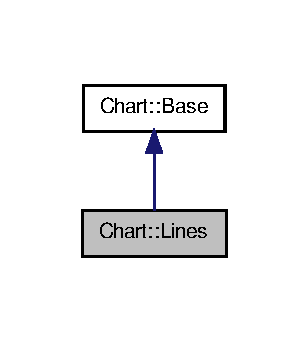
\includegraphics[width=148pt]{classChart_1_1Lines__inherit__graph}
\end{center}
\end{figure}


Collaboration diagram for Chart::Lines:\nopagebreak
\begin{figure}[H]
\begin{center}
\leavevmode
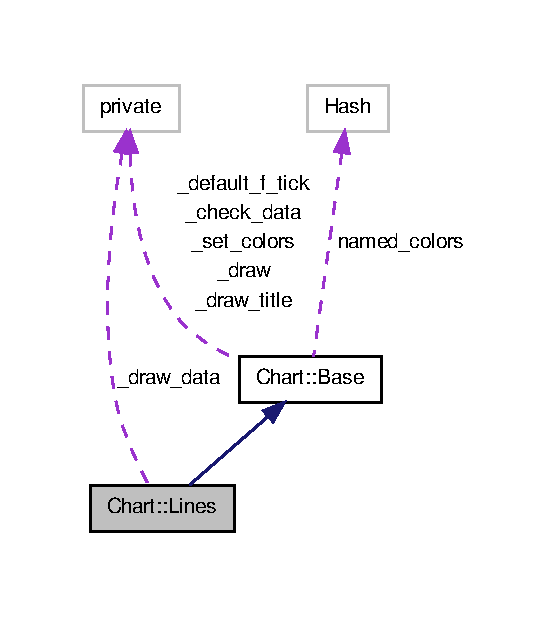
\includegraphics[width=303pt]{classChart_1_1Lines__coll__graph}
\end{center}
\end{figure}
\subsection*{Private Object Methods}
\label{_amgrp57eb0ba2c0003ce1a95a820bfa03b4b4}
 \begin{DoxyCompactItemize}
\item 
\hypertarget{classChart_1_1Lines_aa183fac10f5ac76e314817643a6bfe18}{
private \hyperlink{classChart_1_1Lines_aa183fac10f5ac76e314817643a6bfe18}{\_\-draw\_\-data}}
\label{classChart_1_1Lines_aa183fac10f5ac76e314817643a6bfe18}

\begin{DoxyCompactList}\small\item\em finally get around to plotting the data for lines \item\end{DoxyCompactList}\end{DoxyCompactItemize}
\subsection*{Private Functions}
\label{_amgrp8d29cff216bafa3117e21883ea7c6b5f}
 \begin{DoxyCompactItemize}
\item 
private int \hyperlink{classChart_1_1Lines_ac55c4d77eea62f176e623b10d2094041}{\_\-prepare\_\-brush} (scalar color)
\begin{DoxyCompactList}\small\item\em set the gdBrush object to trick GD into drawing fat lines \item\end{DoxyCompactList}\end{DoxyCompactItemize}


\subsection{Detailed Description}
\hyperlink{classChart_1_1Lines}{Lines} class derived from class \hyperlink{classChart_1_1Base}{Base}. This class provides all functions which are specific to lines 

\subsection{Member Function Documentation}
\hypertarget{classChart_1_1Lines_ac55c4d77eea62f176e623b10d2094041}{
\index{Chart::Lines@{Chart::Lines}!\_\-prepare\_\-brush@{\_\-prepare\_\-brush}}
\index{\_\-prepare\_\-brush@{\_\-prepare\_\-brush}!Chart::Lines@{Chart::Lines}}
\subsubsection[{\_\-prepare\_\-brush}]{\setlength{\rightskip}{0pt plus 5cm}private int Chart::Lines::\_\-prepare\_\-brush (
\begin{DoxyParamCaption}
\item[{scalar}]{ color}
\end{DoxyParamCaption}
)}}
\label{classChart_1_1Lines_ac55c4d77eea62f176e623b10d2094041}


set the gdBrush object to trick GD into drawing fat lines 



The documentation for this class was generated from the following file:\begin{DoxyCompactItemize}
\item 
Chart/\hyperlink{Lines_8pm}{Lines.pm}\end{DoxyCompactItemize}

\hypertarget{classChart_1_1LinesPoints}{
\section{Chart::LinesPoints Class Reference}
\label{classChart_1_1LinesPoints}\index{Chart::LinesPoints@{Chart::LinesPoints}}
}


Inheritance diagram for Chart::LinesPoints:\nopagebreak
\begin{figure}[H]
\begin{center}
\leavevmode
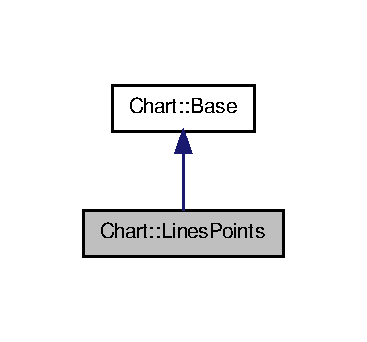
\includegraphics[width=176pt]{classChart_1_1LinesPoints__inherit__graph}
\end{center}
\end{figure}


Collaboration diagram for Chart::LinesPoints:\nopagebreak
\begin{figure}[H]
\begin{center}
\leavevmode
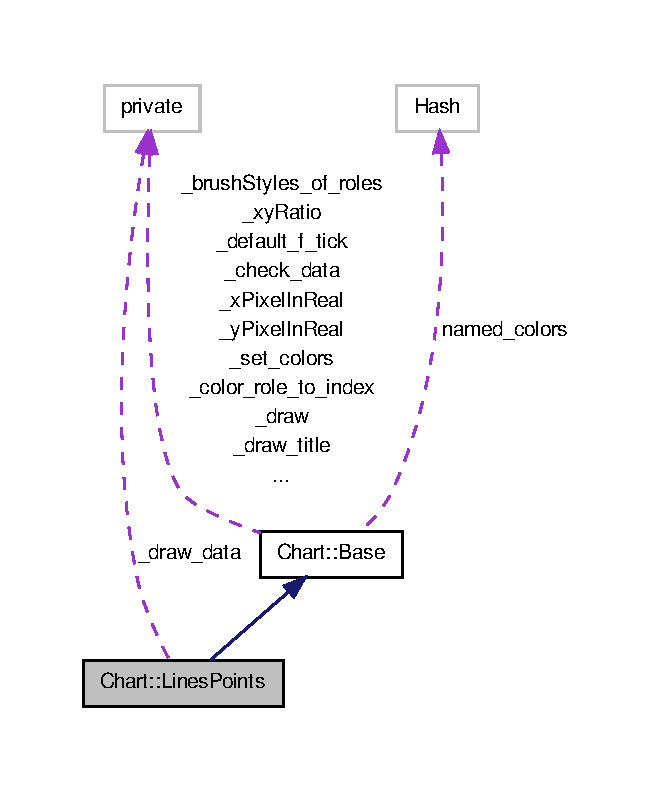
\includegraphics[width=272pt]{classChart_1_1LinesPoints__coll__graph}
\end{center}
\end{figure}
\subsection*{Public Attributes}
\begin{Indent}{\bf Private Functions}\par
{\em \label{_amgrp8d29cff216bafa3117e21883ea7c6b5f}
 }\begin{DoxyCompactItemize}
\item 
\hypertarget{classChart_1_1LinesPoints_a52414c96effaab4189c8488e2ebae742}{
private \hyperlink{classChart_1_1LinesPoints_a52414c96effaab4189c8488e2ebae742}{\_\-draw\_\-data}}
\label{classChart_1_1LinesPoints_a52414c96effaab4189c8488e2ebae742}

\begin{DoxyCompactList}\small\item\em draw the data \item\end{DoxyCompactList}\item 
\hypertarget{classChart_1_1LinesPoints_aaf5def497066928c3c6aa048b847b775}{
private \hyperlink{classChart_1_1LinesPoints_aaf5def497066928c3c6aa048b847b775}{\_\-prepare\_\-brush}}
\label{classChart_1_1LinesPoints_aaf5def497066928c3c6aa048b847b775}

\begin{DoxyCompactList}\small\item\em set the gdBrush object to trick GD into drawing fat lines \item\end{DoxyCompactList}\end{DoxyCompactItemize}
\end{Indent}


The documentation for this class was generated from the following file:\begin{DoxyCompactItemize}
\item 
Chart/\hyperlink{LinesPoints_8pm}{LinesPoints.pm}\end{DoxyCompactItemize}

\hypertarget{classChart_1_1Mountain}{
\section{Chart::Mountain Class Reference}
\label{classChart_1_1Mountain}\index{Chart::Mountain@{Chart::Mountain}}
}


\hyperlink{classChart_1_1Mountain}{Mountain} class derived class for Chart to implement mountain type of plots.  




Inheritance diagram for Chart::Mountain:\nopagebreak
\begin{figure}[H]
\begin{center}
\leavevmode
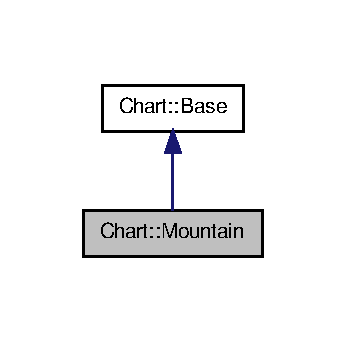
\includegraphics[width=166pt]{classChart_1_1Mountain__inherit__graph}
\end{center}
\end{figure}


Collaboration diagram for Chart::Mountain:\nopagebreak
\begin{figure}[H]
\begin{center}
\leavevmode
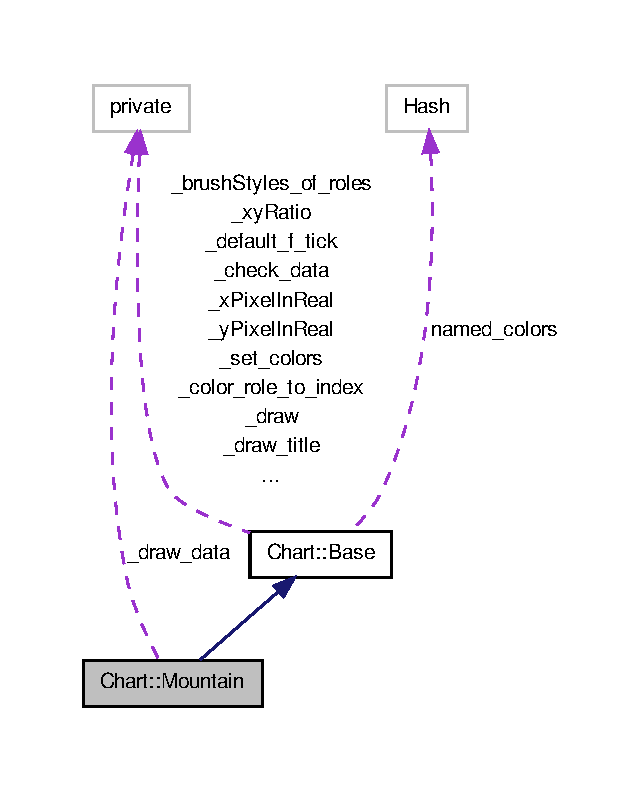
\includegraphics[width=268pt]{classChart_1_1Mountain__coll__graph}
\end{center}
\end{figure}
\subsection*{Private Functions}
\label{_amgrp8d29cff216bafa3117e21883ea7c6b5f}
 \begin{DoxyCompactItemize}
\item 
\hypertarget{classChart_1_1Mountain_aaa146080e4c657cd36cfa2a233955e35}{
private \hyperlink{classChart_1_1Mountain_aaa146080e4c657cd36cfa2a233955e35}{\_\-draw\_\-data}}
\label{classChart_1_1Mountain_aaa146080e4c657cd36cfa2a233955e35}

\begin{DoxyCompactList}\small\item\em draw the data \item\end{DoxyCompactList}\item 
private array \hyperlink{classChart_1_1Mountain_a1da3590b6cb7bc51b8c192e1141a6fa3}{\_\-find\_\-y\_\-range} ()
\begin{DoxyCompactList}\small\item\em Find minimum and maximum value of y data sets. \item\end{DoxyCompactList}\end{DoxyCompactItemize}


\subsection{Detailed Description}
\hyperlink{classChart_1_1Mountain}{Mountain} class derived class for Chart to implement mountain type of plots. Some \hyperlink{classChart_1_1Mountain}{Mountain} chart details:

The effective y data value for a given x point and dataset is the sum of the actual y data values of that dataset and all datasets \char`\"{}below\char`\"{} it (i.e., with higher dataset indexes).

If the y data value in any dataset is undef or negative for a given x, then all datasets are treated as missing for that x.

The y minimum is always forced to zero.

To avoid a dataset area \char`\"{}cutting into\char`\"{} the area of the dataset below it, the y pixel for each dataset point will never be below the y pixel for the same point in the dataset below the dataset. 

\subsection{Member Function Documentation}
\hypertarget{classChart_1_1Mountain_a1da3590b6cb7bc51b8c192e1141a6fa3}{
\index{Chart::Mountain@{Chart::Mountain}!\_\-find\_\-y\_\-range@{\_\-find\_\-y\_\-range}}
\index{\_\-find\_\-y\_\-range@{\_\-find\_\-y\_\-range}!Chart::Mountain@{Chart::Mountain}}
\subsubsection[{\_\-find\_\-y\_\-range}]{\setlength{\rightskip}{0pt plus 5cm}private array Chart::Mountain::\_\-find\_\-y\_\-range (
\begin{DoxyParamCaption}
{}
\end{DoxyParamCaption}
)}}
\label{classChart_1_1Mountain_a1da3590b6cb7bc51b8c192e1141a6fa3}


Find minimum and maximum value of y data sets. 

\begin{DoxyReturn}{Returns}
( min, max, flag\_\-all\_\-integers ) 
\end{DoxyReturn}


Reimplemented from \hyperlink{classChart_1_1Base_ad28e18fc86eebc6846785580977532ca}{Chart::Base}.



The documentation for this class was generated from the following file:\begin{DoxyCompactItemize}
\item 
Chart/\hyperlink{Mountain_8pm}{Mountain.pm}\end{DoxyCompactItemize}

\hypertarget{classChart_1_1Pareto}{
\section{Chart::Pareto Class Reference}
\label{classChart_1_1Pareto}\index{Chart::Pareto@{Chart::Pareto}}
}


\hyperlink{classChart_1_1Pareto}{Pareto} class derived class for Chart to implement.  




Inheritance diagram for Chart::Pareto:\nopagebreak
\begin{figure}[H]
\begin{center}
\leavevmode
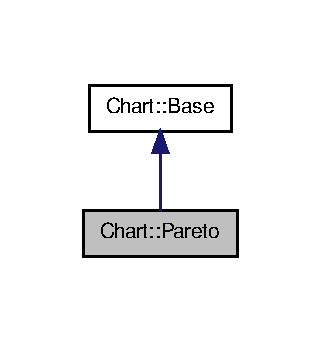
\includegraphics[width=154pt]{classChart_1_1Pareto__inherit__graph}
\end{center}
\end{figure}


Collaboration diagram for Chart::Pareto:\nopagebreak
\begin{figure}[H]
\begin{center}
\leavevmode
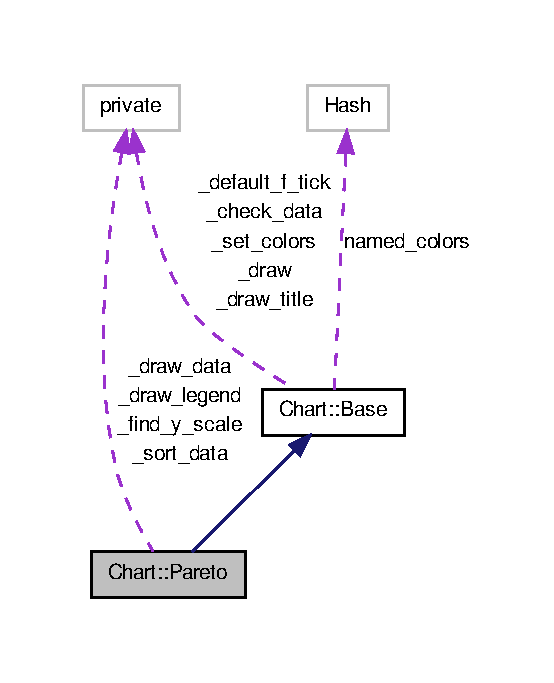
\includegraphics[width=299pt]{classChart_1_1Pareto__coll__graph}
\end{center}
\end{figure}
\subsection*{Private Functions}
\label{_amgrp8d29cff216bafa3117e21883ea7c6b5f}
 \begin{DoxyCompactItemize}
\item 
private \hyperlink{classChart_1_1Pareto_aada3c837beb06c742e78aeb6f7e5c980}{\_\-find\_\-y\_\-scale}
\begin{DoxyCompactList}\small\item\em calculate the range with the sum dataset1. \item\end{DoxyCompactList}\item 
\hypertarget{classChart_1_1Pareto_a83a7720b581c63c2e11a96d78e8d3c14}{
private \hyperlink{classChart_1_1Pareto_a83a7720b581c63c2e11a96d78e8d3c14}{\_\-sort\_\-data}}
\label{classChart_1_1Pareto_a83a7720b581c63c2e11a96d78e8d3c14}

\begin{DoxyCompactList}\small\item\em sort the data \item\end{DoxyCompactList}\item 
\hypertarget{classChart_1_1Pareto_aa6cf49aca8b5b3ac4efd227d06fbebf9}{
private \hyperlink{classChart_1_1Pareto_aa6cf49aca8b5b3ac4efd227d06fbebf9}{\_\-draw\_\-legend}}
\label{classChart_1_1Pareto_aa6cf49aca8b5b3ac4efd227d06fbebf9}

\begin{DoxyCompactList}\small\item\em let them know what all the pretty colors mean \item\end{DoxyCompactList}\item 
\hypertarget{classChart_1_1Pareto_a0e16be0bd97fd6c95bb16fc684e137c7}{
private \hyperlink{classChart_1_1Pareto_a0e16be0bd97fd6c95bb16fc684e137c7}{\_\-draw\_\-data}}
\label{classChart_1_1Pareto_a0e16be0bd97fd6c95bb16fc684e137c7}

\begin{DoxyCompactList}\small\item\em finally get around to plotting the data \item\end{DoxyCompactList}\end{DoxyCompactItemize}


\subsection{Detailed Description}
\hyperlink{classChart_1_1Pareto}{Pareto} class derived class for Chart to implement. 

\subsection{Member Data Documentation}
\hypertarget{classChart_1_1Pareto_aada3c837beb06c742e78aeb6f7e5c980}{
\index{Chart::Pareto@{Chart::Pareto}!\_\-find\_\-y\_\-scale@{\_\-find\_\-y\_\-scale}}
\index{\_\-find\_\-y\_\-scale@{\_\-find\_\-y\_\-scale}!Chart::Pareto@{Chart::Pareto}}
\subsubsection[{\_\-find\_\-y\_\-scale}]{\setlength{\rightskip}{0pt plus 5cm}private {\bf Chart::Pareto::\_\-find\_\-y\_\-scale}}}
\label{classChart_1_1Pareto_aada3c837beb06c742e78aeb6f7e5c980}


calculate the range with the sum dataset1. 

all datas has to be positiv 

The documentation for this class was generated from the following file:\begin{DoxyCompactItemize}
\item 
Chart/\hyperlink{Pareto_8pm}{Pareto.pm}\end{DoxyCompactItemize}

\hypertarget{classChart_1_1Pie}{
\section{Chart::Pie Class Reference}
\label{classChart_1_1Pie}\index{Chart::Pie@{Chart::Pie}}
}


\hyperlink{classChart_1_1Pie}{Pie} class derived class for Chart to implement pies.  




Inheritance diagram for Chart::Pie:\nopagebreak
\begin{figure}[H]
\begin{center}
\leavevmode
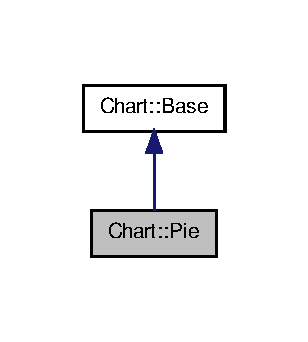
\includegraphics[width=148pt]{classChart_1_1Pie__inherit__graph}
\end{center}
\end{figure}


Collaboration diagram for Chart::Pie:\nopagebreak
\begin{figure}[H]
\begin{center}
\leavevmode
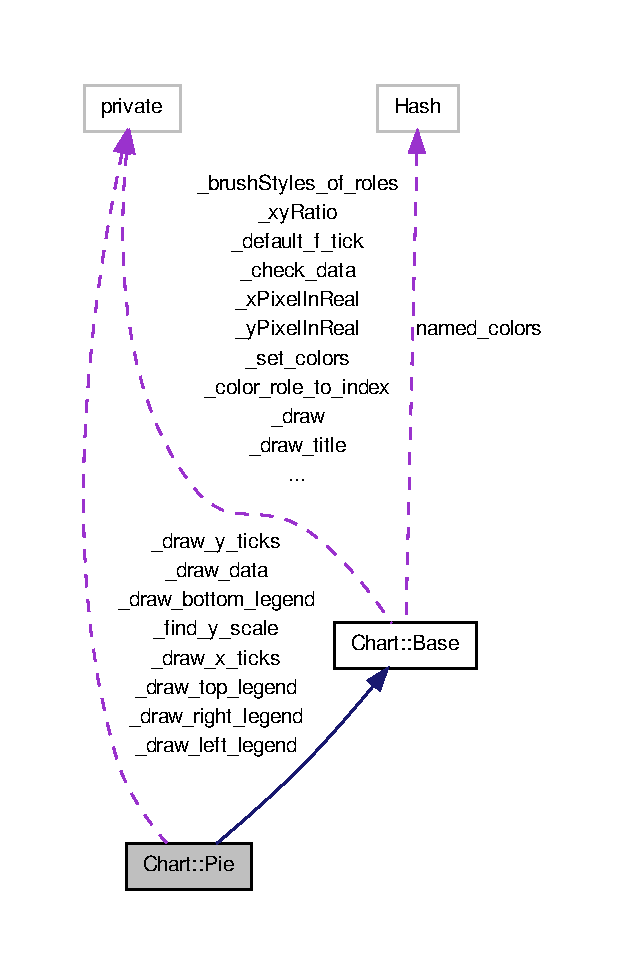
\includegraphics[width=289pt]{classChart_1_1Pie__coll__graph}
\end{center}
\end{figure}
\subsection*{Private Functions}
\label{_amgrp8d29cff216bafa3117e21883ea7c6b5f}
 \begin{DoxyCompactItemize}
\item 
private \hyperlink{classChart_1_1Pie_a223df30ed6555878015b643547919911}{\_\-draw\_\-data}
\begin{DoxyCompactList}\small\item\em finally get around to plotting the data \item\end{DoxyCompactList}\item 
\hypertarget{classChart_1_1Pie_a382ad440d989138b4407473660cc0049}{
private \hyperlink{classChart_1_1Pie_a382ad440d989138b4407473660cc0049}{\_\-draw\_\-right\_\-legend}}
\label{classChart_1_1Pie_a382ad440d989138b4407473660cc0049}

\begin{DoxyCompactList}\small\item\em Overwrite the legend methods to get the right legend. \item\end{DoxyCompactList}\item 
\hypertarget{classChart_1_1Pie_a2cb3d178f0140da6e9d65bde7bd66563}{
private \hyperlink{classChart_1_1Pie_a2cb3d178f0140da6e9d65bde7bd66563}{\_\-draw\_\-left\_\-legend}}
\label{classChart_1_1Pie_a2cb3d178f0140da6e9d65bde7bd66563}

\begin{DoxyCompactList}\small\item\em put the legend on the left of the chart \item\end{DoxyCompactList}\item 
\hypertarget{classChart_1_1Pie_a4784e7e03796ecef3126fc505fa1e992}{
private \hyperlink{classChart_1_1Pie_a4784e7e03796ecef3126fc505fa1e992}{\_\-draw\_\-bottom\_\-legend}}
\label{classChart_1_1Pie_a4784e7e03796ecef3126fc505fa1e992}

\begin{DoxyCompactList}\small\item\em put the legend on the bottom of the chart \item\end{DoxyCompactList}\item 
\hypertarget{classChart_1_1Pie_acf7d23aa043e7ecc4aa1fcd4c80f9d9e}{
private \hyperlink{classChart_1_1Pie_acf7d23aa043e7ecc4aa1fcd4c80f9d9e}{\_\-draw\_\-top\_\-legend}}
\label{classChart_1_1Pie_acf7d23aa043e7ecc4aa1fcd4c80f9d9e}

\begin{DoxyCompactList}\small\item\em put the legend on top of the chart \item\end{DoxyCompactList}\item 
private \hyperlink{classChart_1_1Pie_ac4809da05e978fb109873de806d75b35}{\_\-draw\_\-x\_\-ticks}
\begin{DoxyCompactList}\small\item\em Override the ticks methods for the pie charts. \item\end{DoxyCompactList}\item 
private \hyperlink{classChart_1_1Pie_adaf9a2d4a6b552f205e3455b61c687cb}{\_\-draw\_\-y\_\-ticks}
\begin{DoxyCompactList}\small\item\em Override the ticks methods for the pie charts. \item\end{DoxyCompactList}\item 
private \hyperlink{classChart_1_1Pie_ae2d77fbce88ae7e1a9e37b8a5cdcb5cb}{\_\-find\_\-y\_\-scale}
\begin{DoxyCompactList}\small\item\em Override the find\_\-y\_\-scale methods for the pie charts. \item\end{DoxyCompactList}\end{DoxyCompactItemize}


\subsection{Detailed Description}
\hyperlink{classChart_1_1Pie}{Pie} class derived class for Chart to implement pies. 

\subsection{Member Data Documentation}
\hypertarget{classChart_1_1Pie_a223df30ed6555878015b643547919911}{
\index{Chart::Pie@{Chart::Pie}!\_\-draw\_\-data@{\_\-draw\_\-data}}
\index{\_\-draw\_\-data@{\_\-draw\_\-data}!Chart::Pie@{Chart::Pie}}
\subsubsection[{\_\-draw\_\-data}]{\setlength{\rightskip}{0pt plus 5cm}private {\bf Chart::Pie::\_\-draw\_\-data}}}
\label{classChart_1_1Pie_a223df30ed6555878015b643547919911}


finally get around to plotting the data 

The user may define the kind of labelling the data by setting\par
 'label\_\-values' to 'percent' if she wants to have the percentages\par
 'label\_\-values' to 'values' if she wants to have the absolut values\par
 'label\_\-values' to 'both' if she wants to have absolut values and percentages\par
 'label\_\-values' to 'none' if she wants to have neither absolute values nor percentages\par
 'ring' to a number less then 1 to define a ring as output; if 'ring' is 1 ore greater a full pie is plotted\par
 \hypertarget{classChart_1_1Pie_ac4809da05e978fb109873de806d75b35}{
\index{Chart::Pie@{Chart::Pie}!\_\-draw\_\-x\_\-ticks@{\_\-draw\_\-x\_\-ticks}}
\index{\_\-draw\_\-x\_\-ticks@{\_\-draw\_\-x\_\-ticks}!Chart::Pie@{Chart::Pie}}
\subsubsection[{\_\-draw\_\-x\_\-ticks}]{\setlength{\rightskip}{0pt plus 5cm}private {\bf Chart::Pie::\_\-draw\_\-x\_\-ticks}}}
\label{classChart_1_1Pie_ac4809da05e978fb109873de806d75b35}


Override the ticks methods for the pie charts. 

\par
 Here: do nothing \hypertarget{classChart_1_1Pie_adaf9a2d4a6b552f205e3455b61c687cb}{
\index{Chart::Pie@{Chart::Pie}!\_\-draw\_\-y\_\-ticks@{\_\-draw\_\-y\_\-ticks}}
\index{\_\-draw\_\-y\_\-ticks@{\_\-draw\_\-y\_\-ticks}!Chart::Pie@{Chart::Pie}}
\subsubsection[{\_\-draw\_\-y\_\-ticks}]{\setlength{\rightskip}{0pt plus 5cm}private {\bf Chart::Pie::\_\-draw\_\-y\_\-ticks}}}
\label{classChart_1_1Pie_adaf9a2d4a6b552f205e3455b61c687cb}


Override the ticks methods for the pie charts. 

\par
 \hypertarget{classChart_1_1Pie_ae2d77fbce88ae7e1a9e37b8a5cdcb5cb}{
\index{Chart::Pie@{Chart::Pie}!\_\-find\_\-y\_\-scale@{\_\-find\_\-y\_\-scale}}
\index{\_\-find\_\-y\_\-scale@{\_\-find\_\-y\_\-scale}!Chart::Pie@{Chart::Pie}}
\subsubsection[{\_\-find\_\-y\_\-scale}]{\setlength{\rightskip}{0pt plus 5cm}private {\bf Chart::Pie::\_\-find\_\-y\_\-scale}}}
\label{classChart_1_1Pie_ae2d77fbce88ae7e1a9e37b8a5cdcb5cb}


Override the find\_\-y\_\-scale methods for the pie charts. 

\par
 Here: do nothing 

The documentation for this class was generated from the following file:\begin{DoxyCompactItemize}
\item 
Chart/\hyperlink{Pie_8pm}{Pie.pm}\end{DoxyCompactItemize}

\hypertarget{classChart_1_1Points}{
\section{Chart::Points Class Reference}
\label{classChart_1_1Points}\index{Chart::Points@{Chart::Points}}
}


\hyperlink{classChart_1_1Points}{Points} class derived from class \hyperlink{classChart_1_1Base}{Base}.  




Inheritance diagram for Chart::Points:\nopagebreak
\begin{figure}[H]
\begin{center}
\leavevmode
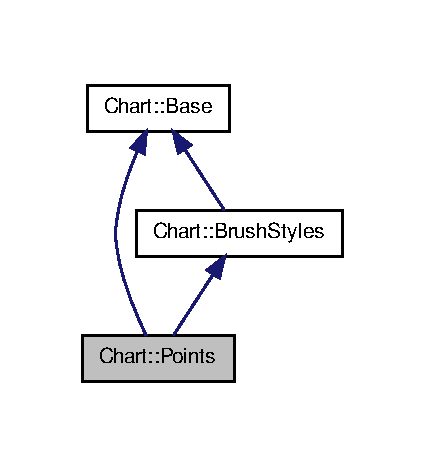
\includegraphics[width=152pt]{classChart_1_1Points__inherit__graph}
\end{center}
\end{figure}


Collaboration diagram for Chart::Points:\nopagebreak
\begin{figure}[H]
\begin{center}
\leavevmode
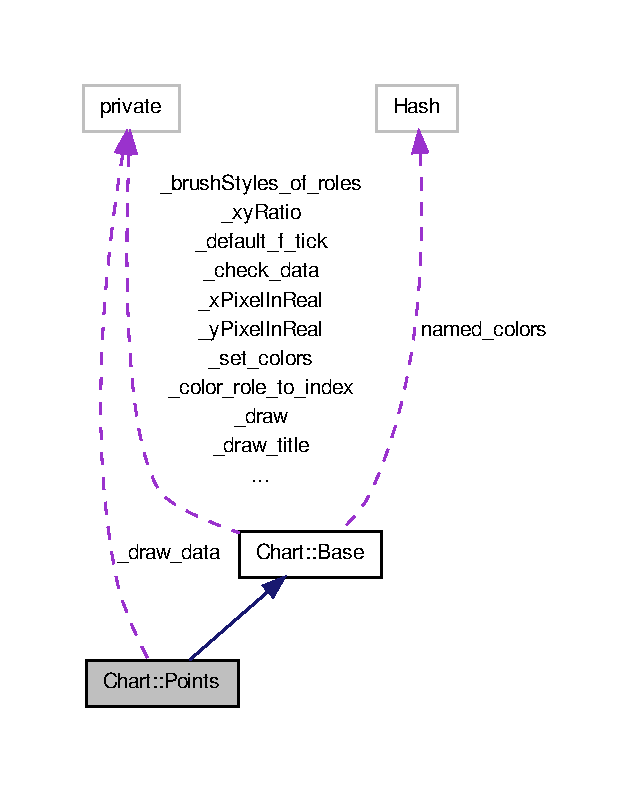
\includegraphics[width=303pt]{classChart_1_1Points__coll__graph}
\end{center}
\end{figure}
\subsection*{Private Functions}
\label{_amgrp8d29cff216bafa3117e21883ea7c6b5f}
 \begin{DoxyCompactItemize}
\item 
\hypertarget{classChart_1_1Points_afabf6460cdf4056cdbef97146941f671}{
private \hyperlink{classChart_1_1Points_afabf6460cdf4056cdbef97146941f671}{\_\-draw\_\-data}}
\label{classChart_1_1Points_afabf6460cdf4056cdbef97146941f671}

\begin{DoxyCompactList}\small\item\em finally get around to plotting the data \item\end{DoxyCompactList}\end{DoxyCompactItemize}


\subsection{Detailed Description}
\hyperlink{classChart_1_1Points}{Points} class derived from class \hyperlink{classChart_1_1Base}{Base}. This class provides all functions which are specific to points 

The documentation for this class was generated from the following file:\begin{DoxyCompactItemize}
\item 
Chart/\hyperlink{Points_8pm}{Points.pm}\end{DoxyCompactItemize}

\hypertarget{classChart_1_1Split}{
\section{Chart::Split Class Reference}
\label{classChart_1_1Split}\index{Chart::Split@{Chart::Split}}
}


\hyperlink{classChart_1_1Split}{Split} class derived from class \hyperlink{classChart_1_1Base}{Base}.  




Inheritance diagram for Chart::Split:\nopagebreak
\begin{figure}[H]
\begin{center}
\leavevmode
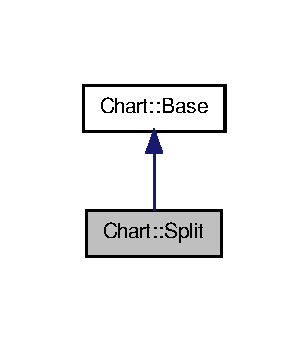
\includegraphics[width=148pt]{classChart_1_1Split__inherit__graph}
\end{center}
\end{figure}


Collaboration diagram for Chart::Split:\nopagebreak
\begin{figure}[H]
\begin{center}
\leavevmode
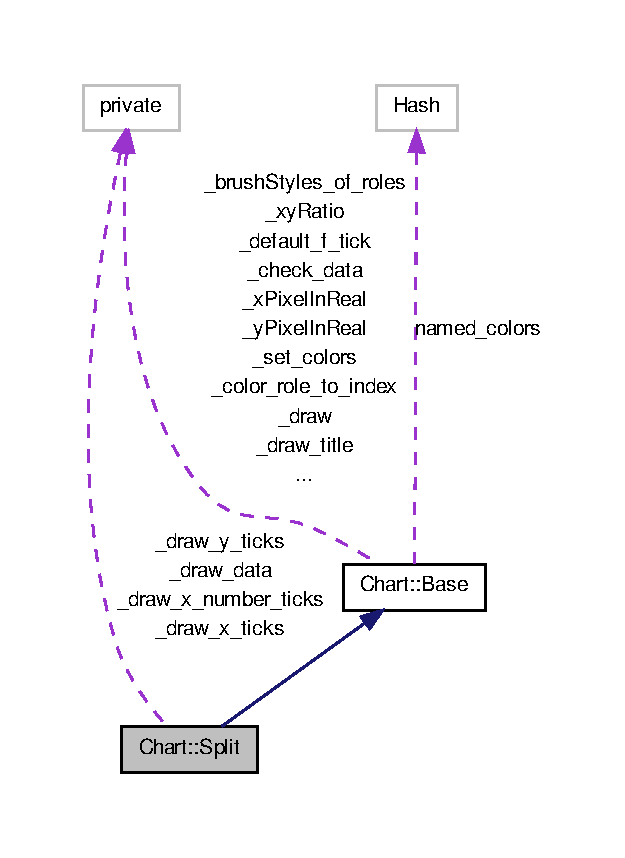
\includegraphics[width=291pt]{classChart_1_1Split__coll__graph}
\end{center}
\end{figure}
\subsection*{Private Functions}
\label{_amgrp8d29cff216bafa3117e21883ea7c6b5f}
 \begin{DoxyCompactItemize}
\item 
\hypertarget{classChart_1_1Split_a9acbd65cad87e7571b02687e9efbe2dd}{
private \hyperlink{classChart_1_1Split_a9acbd65cad87e7571b02687e9efbe2dd}{\_\-draw\_\-x\_\-number\_\-ticks}}
\label{classChart_1_1Split_a9acbd65cad87e7571b02687e9efbe2dd}

\begin{DoxyCompactList}\small\item\em draw the ticks \item\end{DoxyCompactList}\item 
\hypertarget{classChart_1_1Split_af95c5609fac7bd93d85c3f43db943e21}{
private \hyperlink{classChart_1_1Split_af95c5609fac7bd93d85c3f43db943e21}{\_\-draw\_\-x\_\-ticks}}
\label{classChart_1_1Split_af95c5609fac7bd93d85c3f43db943e21}

\begin{DoxyCompactList}\small\item\em override the function implemented in base \item\end{DoxyCompactList}\item 
\hypertarget{classChart_1_1Split_a01d9dbce6162528c77c407000a7267f2}{
private \hyperlink{classChart_1_1Split_a01d9dbce6162528c77c407000a7267f2}{\_\-draw\_\-y\_\-ticks}}
\label{classChart_1_1Split_a01d9dbce6162528c77c407000a7267f2}

\begin{DoxyCompactList}\small\item\em override the function implemented in base \item\end{DoxyCompactList}\item 
\hypertarget{classChart_1_1Split_a7194ba0840dbc7d699c0582b61e9cb80}{
private \hyperlink{classChart_1_1Split_a7194ba0840dbc7d699c0582b61e9cb80}{\_\-draw\_\-data}}
\label{classChart_1_1Split_a7194ba0840dbc7d699c0582b61e9cb80}

\begin{DoxyCompactList}\small\item\em plot the data \item\end{DoxyCompactList}\end{DoxyCompactItemize}


\subsection{Detailed Description}
\hyperlink{classChart_1_1Split}{Split} class derived from class \hyperlink{classChart_1_1Base}{Base}. This class provides all functions which are specific to splitted plots 

The documentation for this class was generated from the following file:\begin{DoxyCompactItemize}
\item 
Chart/\hyperlink{Split_8pm}{Split.pm}\end{DoxyCompactItemize}

\hypertarget{classChart_1_1StackedBars}{
\section{Chart::StackedBars Class Reference}
\label{classChart_1_1StackedBars}\index{Chart::StackedBars@{Chart::StackedBars}}
}


\hyperlink{classChart_1_1StackedBars}{StackedBars} class derived from class \hyperlink{classChart_1_1Base}{Base}.  




Inheritance diagram for Chart::StackedBars:\nopagebreak
\begin{figure}[H]
\begin{center}
\leavevmode
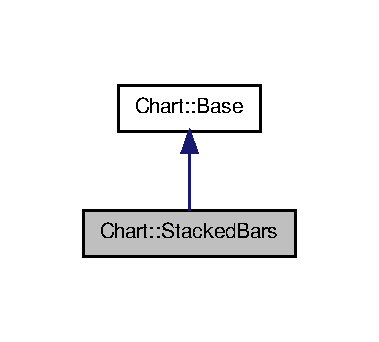
\includegraphics[width=182pt]{classChart_1_1StackedBars__inherit__graph}
\end{center}
\end{figure}


Collaboration diagram for Chart::StackedBars:\nopagebreak
\begin{figure}[H]
\begin{center}
\leavevmode
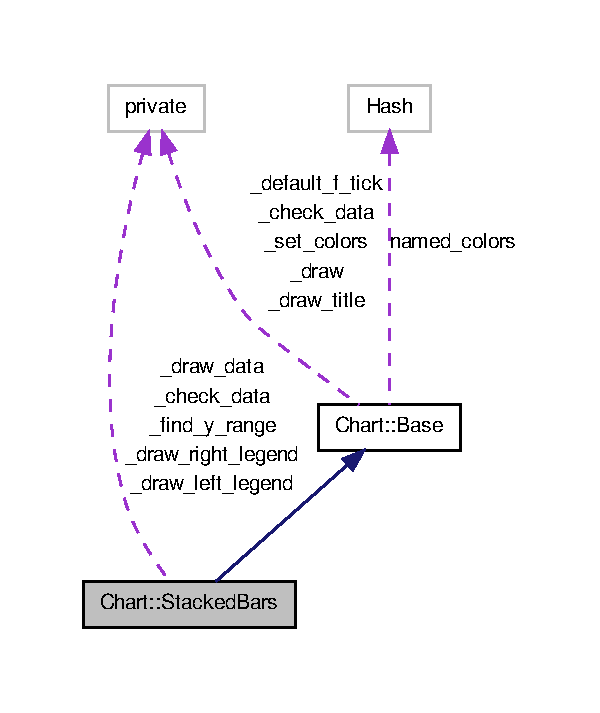
\includegraphics[width=302pt]{classChart_1_1StackedBars__coll__graph}
\end{center}
\end{figure}
\subsection*{Private Functions}
\label{_amgrp8d29cff216bafa3117e21883ea7c6b5f}
 \begin{DoxyCompactItemize}
\item 
\hypertarget{classChart_1_1StackedBars_a8d772463780f75cc985ae890ad8a94d1}{
private \hyperlink{classChart_1_1StackedBars_a8d772463780f75cc985ae890ad8a94d1}{\_\-check\_\-data}}
\label{classChart_1_1StackedBars_a8d772463780f75cc985ae890ad8a94d1}

\begin{DoxyCompactList}\small\item\em override check\_\-data to make sure we don't get datasets with positive and negative values mixed \item\end{DoxyCompactList}\item 
\hypertarget{classChart_1_1StackedBars_a3b2346b67bdcae53e756dc29bb0cf748}{
private {\bfseries \_\-find\_\-y\_\-range}}
\label{classChart_1_1StackedBars_a3b2346b67bdcae53e756dc29bb0cf748}

\item 
\hypertarget{classChart_1_1StackedBars_abacb5ba7afd1090c229d8f0ba9a56ddb}{
private \hyperlink{classChart_1_1StackedBars_abacb5ba7afd1090c229d8f0ba9a56ddb}{\_\-draw\_\-data}}
\label{classChart_1_1StackedBars_abacb5ba7afd1090c229d8f0ba9a56ddb}

\begin{DoxyCompactList}\small\item\em finally get around to plotting the data \item\end{DoxyCompactList}\item 
\hypertarget{classChart_1_1StackedBars_a7138f939a7d0f5c21a53bee45939717c}{
private {\bfseries \_\-draw\_\-left\_\-legend}}
\label{classChart_1_1StackedBars_a7138f939a7d0f5c21a53bee45939717c}

\item 
\hypertarget{classChart_1_1StackedBars_aad01909f5d3a6af9e014926f2a026014}{
private {\bfseries \_\-draw\_\-right\_\-legend}}
\label{classChart_1_1StackedBars_aad01909f5d3a6af9e014926f2a026014}

\end{DoxyCompactItemize}


\subsection{Detailed Description}
\hyperlink{classChart_1_1StackedBars}{StackedBars} class derived from class \hyperlink{classChart_1_1Base}{Base}. This class provides all functions which are specific to stacked bars 

The documentation for this class was generated from the following file:\begin{DoxyCompactItemize}
\item 
Chart/\hyperlink{StackedBars_8pm}{StackedBars.pm}\end{DoxyCompactItemize}

\chapter{File Documentation}
\hypertarget{Bars_8pm}{
\section{Chart/Bars.pm File Reference}
\label{Bars_8pm}\index{Chart/Bars.pm@{Chart/Bars.pm}}
}


Implementation of \hyperlink{classChart_1_1Bars}{Chart::Bars}.  


\subsection*{Classes}
\begin{DoxyCompactItemize}
\item 
class \hyperlink{classChart_1_1Bars}{Chart::Bars}
\begin{DoxyCompactList}\small\item\em \hyperlink{classChart_1_1Bars}{Bars} class provides all functions which are specific to vertical bars. \item\end{DoxyCompactList}\end{DoxyCompactItemize}


\subsection{Detailed Description}
Implementation of \hyperlink{classChart_1_1Bars}{Chart::Bars}. written by \begin{DoxyAuthor}{Author}
david bonner (\href{mailto:dbonner@cs.bu.edu}{\tt dbonner@cs.bu.edu})
\end{DoxyAuthor}
maintained by the \begin{DoxyAuthor}{Author}
Chart Group at Geodetic Fundamental Station Wettzell (\href{mailto:Chart@fs.wettzell.de}{\tt Chart@fs.wettzell.de}) 
\end{DoxyAuthor}
\begin{DoxyDate}{Date}
2012-\/01-\/06 
\end{DoxyDate}
\begin{DoxyVersion}{Version}
2.4.4 
\end{DoxyVersion}

\hypertarget{Base_8pm}{
\section{Chart/Base.pm File Reference}
\label{Base_8pm}\index{Chart/Base.pm@{Chart/Base.pm}}
}


Implementation of \hyperlink{classChart_1_1Base}{Chart::Base}.  


\subsection*{Classes}
\begin{DoxyCompactItemize}
\item 
class \hyperlink{classChart_1_1Base}{Chart::Base}
\begin{DoxyCompactList}\small\item\em \hyperlink{classChart_1_1Base}{Base} class for Chart; all other classes derived from here. \item\end{DoxyCompactList}\end{DoxyCompactItemize}


\subsection{Detailed Description}
Implementation of \hyperlink{classChart_1_1Base}{Chart::Base}. written by \begin{DoxyAuthor}{Author}
david bonner (\href{mailto:dbonner@cs.bu.edu}{\tt dbonner@cs.bu.edu})
\end{DoxyAuthor}
maintained by the \begin{DoxyAuthor}{Author}
Chart Group at Geodetic Fundamental Station Wettzell (\href{mailto:Chart@fs.wettzell.de}{\tt Chart@fs.wettzell.de}) 
\end{DoxyAuthor}
\begin{DoxyDate}{Date}
2012-\/01-\/06 
\end{DoxyDate}
\begin{DoxyVersion}{Version}
2.4.4 
\end{DoxyVersion}

\hypertarget{BrushStyles_8pm}{
\section{Chart/BrushStyles.pm File Reference}
\label{BrushStyles_8pm}\index{Chart/BrushStyles.pm@{Chart/BrushStyles.pm}}
}


\hyperlink{classChart_1_1BrushStyles}{Chart::BrushStyles}.  


\subsection*{Classes}
\begin{DoxyCompactItemize}
\item 
class \hyperlink{classChart_1_1BrushStyles}{Chart::BrushStyles}
\begin{DoxyCompactList}\small\item\em Define styles for \hyperlink{classChart_1_1Points}{Points} and \hyperlink{classChart_1_1LinesPoints}{LinesPoints} classes. \item\end{DoxyCompactList}\end{DoxyCompactItemize}


\subsection{Detailed Description}
\hyperlink{classChart_1_1BrushStyles}{Chart::BrushStyles}. written and maintained by the \begin{DoxyAuthor}{Author}
Chart Group at Geodetic Fundamental Station Wettzell (\href{mailto:Chart@fs.wettzell.de}{\tt Chart@fs.wettzell.de}) 
\end{DoxyAuthor}
\begin{DoxyDate}{Date}
2011-\/11-\/25 
\end{DoxyDate}
\begin{DoxyVersion}{Version}
2.4.3 
\end{DoxyVersion}

\hypertarget{Composite_8pm}{
\section{Chart/Composite.pm File Reference}
\label{Composite_8pm}\index{Chart/Composite.pm@{Chart/Composite.pm}}
}


Implementation of \hyperlink{classChart_1_1Composite}{Chart::Composite}.  


\subsection*{Classes}
\begin{DoxyCompactItemize}
\item 
class \hyperlink{classChart_1_1Composite}{Chart::Composite}
\begin{DoxyCompactList}\small\item\em \hyperlink{classChart_1_1Composite}{Composite} class derived from class \hyperlink{classChart_1_1Base}{Base}. \item\end{DoxyCompactList}\item 
class \hyperlink{classChart_1_1Composite}{Chart::Composite}
\begin{DoxyCompactList}\small\item\em \hyperlink{classChart_1_1Composite}{Composite} class derived from class \hyperlink{classChart_1_1Base}{Base}. \item\end{DoxyCompactList}\end{DoxyCompactItemize}


\subsection{Detailed Description}
Implementation of \hyperlink{classChart_1_1Composite}{Chart::Composite}. written by \begin{DoxyAuthor}{Author}
david bonner (\href{mailto:dbonner@cs.bu.edu}{\tt dbonner@cs.bu.edu})
\end{DoxyAuthor}
maintained by the \begin{DoxyAuthor}{Author}
Chart Group at Geodetic Fundamental Station Wettzell (\href{mailto:Chart@fs.wettzell.de}{\tt Chart@fs.wettzell.de}) 
\end{DoxyAuthor}
\begin{DoxyDate}{Date}
2011-\/11-\/25 
\end{DoxyDate}
\begin{DoxyVersion}{Version}
2.4.3
\end{DoxyVersion}
-\/-\/-\/-\/-\/-\/-\/-\/-\/-\/-\/-\/-\/-\/-\/-\/-\/-\/-\/-\/-\/-\/-\/-\/-\/-\/-\/-\/-\/-\/-\/-\/-\/-\/-\/-\/-\/-\/-\/-\/-\/-\/-\/-\/-\/-\/-\/-\/-\/-\/-\/-\/-\/-\/-\/-\/-\/-\/-\/-\/-\/-\/-\/-\/-\/-\/-\/-\/-\/ History: -\/-\/-\/-\/-\/-\/-\/-\/-\/-\/ 
\hypertarget{Constants_8pm}{
\section{Chart/Constants.pm File Reference}
\label{Constants_8pm}\index{Chart/Constants.pm@{Chart/Constants.pm}}
}


Constants used in Chart:\par
 PI.  


\subsection*{Classes}
\begin{DoxyCompactItemize}
\item 
class \hyperlink{classChart_1_1Constants}{Chart::Constants}
\begin{DoxyCompactList}\small\item\em \hyperlink{classChart_1_1Constants}{Constants} class defines all necessary constants for Class Chart. \item\end{DoxyCompactList}\end{DoxyCompactItemize}


\subsection{Detailed Description}
Constants used in Chart:\par
 PI. written and maintained by \begin{DoxyAuthor}{Author}
Chart Group at Geodetic Fundamental Station Wettzell (\href{mailto:Chart@fs.wettzell.de}{\tt Chart@fs.wettzell.de}) 
\end{DoxyAuthor}
\begin{DoxyDate}{Date}
2012-\/01-\/06 
\end{DoxyDate}
\begin{DoxyVersion}{Version}
2.4.4 
\end{DoxyVersion}

\hypertarget{Direction_8pm}{
\section{Chart/Direction.pm File Reference}
\label{Direction_8pm}\index{Chart/Direction.pm@{Chart/Direction.pm}}
}


Implementation of \hyperlink{classChart_1_1Direction}{Chart::Direction}.  


\subsection*{Classes}
\begin{DoxyCompactItemize}
\item 
class \hyperlink{classChart_1_1Direction}{Chart::Direction}
\begin{DoxyCompactList}\small\item\em \hyperlink{classChart_1_1Direction}{Direction} class derived class for Chart to implement direction charts. \item\end{DoxyCompactList}\item 
class \hyperlink{classChart_1_1Direction}{Chart::Direction}
\begin{DoxyCompactList}\small\item\em \hyperlink{classChart_1_1Direction}{Direction} class derived class for Chart to implement direction charts. \item\end{DoxyCompactList}\end{DoxyCompactItemize}


\subsection{Detailed Description}
Implementation of \hyperlink{classChart_1_1Direction}{Chart::Direction}. written by \begin{DoxyAuthor}{Author}
Chart Group at Geodetic Fundamental Station Wettzell (\href{mailto:Chart@fs.wettzell.de}{\tt Chart@fs.wettzell.de}) 
\end{DoxyAuthor}
\begin{DoxyDate}{Date}
2011-\/11-\/25 
\end{DoxyDate}
\begin{DoxyVersion}{Version}
2.4.3 
\end{DoxyVersion}

\hypertarget{ErrorBars_8pm}{
\section{Chart/ErrorBars.pm File Reference}
\label{ErrorBars_8pm}\index{Chart/ErrorBars.pm@{Chart/ErrorBars.pm}}
}


Implementation of \hyperlink{classChart_1_1ErrorBars}{Chart::ErrorBars}.  


\subsection*{Classes}
\begin{DoxyCompactItemize}
\item 
class \hyperlink{classChart_1_1ErrorBars}{Chart::ErrorBars}
\begin{DoxyCompactList}\small\item\em \hyperlink{classChart_1_1ErrorBars}{ErrorBars} class derived from class \hyperlink{classChart_1_1Base}{Base}. \item\end{DoxyCompactList}\item 
class \hyperlink{classChart_1_1ErrorBars}{Chart::ErrorBars}
\begin{DoxyCompactList}\small\item\em \hyperlink{classChart_1_1ErrorBars}{ErrorBars} class derived from class \hyperlink{classChart_1_1Base}{Base}. \item\end{DoxyCompactList}\end{DoxyCompactItemize}


\subsection{Detailed Description}
Implementation of \hyperlink{classChart_1_1ErrorBars}{Chart::ErrorBars}. written by \begin{DoxyAuthor}{Author}
david bonner (\href{mailto:dbonner@cs.bu.edu}{\tt dbonner@cs.bu.edu})
\end{DoxyAuthor}
maintained by the \begin{DoxyAuthor}{Author}
Chart Group at Geodetic Fundamental Station Wettzell (\href{mailto:Chart@fs.wettzell.de}{\tt Chart@fs.wettzell.de}) 
\end{DoxyAuthor}
\begin{DoxyDate}{Date}
2012-\/01-\/06 
\end{DoxyDate}
\begin{DoxyVersion}{Version}
2.4.4 
\end{DoxyVersion}

\hypertarget{HorizontalBars_8pm}{
\section{Chart/HorizontalBars.pm File Reference}
\label{HorizontalBars_8pm}\index{Chart/HorizontalBars.pm@{Chart/HorizontalBars.pm}}
}


Implementation of \hyperlink{classChart_1_1HorizontalBars}{Chart::HorizontalBars}.  


\subsection*{Classes}
\begin{DoxyCompactItemize}
\item 
class \hyperlink{classChart_1_1HorizontalBars}{Chart::HorizontalBars}
\begin{DoxyCompactList}\small\item\em \hyperlink{classChart_1_1Bars}{Bars} class derived from class \hyperlink{classChart_1_1Base}{Base}. \item\end{DoxyCompactList}\end{DoxyCompactItemize}


\subsection{Detailed Description}
Implementation of \hyperlink{classChart_1_1HorizontalBars}{Chart::HorizontalBars}. maintained and written by the \begin{DoxyAuthor}{Author}
Chart Group at Geodetic Fundamental Station Wettzell (\href{mailto:Chart@fs.wettzell.de}{\tt Chart@fs.wettzell.de}) 
\end{DoxyAuthor}
\begin{DoxyDate}{Date}
2011-\/11-\/25 
\end{DoxyDate}
\begin{DoxyVersion}{Version}
2.4.3 
\end{DoxyVersion}

\hypertarget{Lines_8pm}{
\section{Chart/Lines.pm File Reference}
\label{Lines_8pm}\index{Chart/Lines.pm@{Chart/Lines.pm}}
}


Implementation of \hyperlink{classChart_1_1Lines}{Chart::Lines}.  


\subsection*{Classes}
\begin{DoxyCompactItemize}
\item 
class \hyperlink{classChart_1_1Lines}{Chart::Lines}
\begin{DoxyCompactList}\small\item\em \hyperlink{classChart_1_1Bars}{Bars} class derived from class \hyperlink{classChart_1_1Base}{Base}. \item\end{DoxyCompactList}\end{DoxyCompactItemize}


\subsection{Detailed Description}
Implementation of \hyperlink{classChart_1_1Lines}{Chart::Lines}. written by david bonner \href{mailto:dbonner@cs.bu.edu}{\tt dbonner@cs.bu.edu}

maintained by the Chart Group at Geodetic Fundamental Station Wettzell \href{mailto:Chart@fs.wettzell.de}{\tt Chart@fs.wettzell.de} \begin{DoxyAuthor}{Author}
Chart Group (\href{mailto:Chart@fs.wettzell.de}{\tt Chart@fs.wettzell.de}) 
\end{DoxyAuthor}
\begin{DoxyDate}{Date}
2011-\/11-\/25 
\end{DoxyDate}
\begin{DoxyVersion}{Version}
2.4.3 
\end{DoxyVersion}

\hypertarget{LinesPoints_8pm}{
\section{Chart/LinesPoints.pm File Reference}
\label{LinesPoints_8pm}\index{Chart/LinesPoints.pm@{Chart/LinesPoints.pm}}
}


Implementation of \hyperlink{classChart_1_1LinesPoints}{Chart::LinesPoints}.  


\subsection*{Classes}
\begin{DoxyCompactItemize}
\item 
class \hyperlink{classChart_1_1LinesPoints}{Chart::LinesPoints}
\end{DoxyCompactItemize}


\subsection{Detailed Description}
Implementation of \hyperlink{classChart_1_1LinesPoints}{Chart::LinesPoints}. written by \begin{DoxyAuthor}{Author}
david bonner (\href{mailto:dbonner@cs.bu.edu}{\tt dbonner@cs.bu.edu})
\end{DoxyAuthor}
maintained by the \begin{DoxyAuthor}{Author}
Chart Group at Geodetic Fundamental Station Wettzell (\href{mailto:Chart@fs.wettzell.de}{\tt Chart@fs.wettzell.de}) 
\end{DoxyAuthor}
\begin{DoxyDate}{Date}
2011-\/11-\/25 
\end{DoxyDate}
\begin{DoxyVersion}{Version}
2.4.3 
\end{DoxyVersion}

\hypertarget{Mountain_8pm}{
\section{Chart/Mountain.pm File Reference}
\label{Mountain_8pm}\index{Chart/Mountain.pm@{Chart/Mountain.pm}}
}


Implementation of \hyperlink{classChart_1_1Mountain}{Chart::Mountain}.  


\subsection*{Classes}
\begin{DoxyCompactItemize}
\item 
class \hyperlink{classChart_1_1Mountain}{Chart::Mountain}
\begin{DoxyCompactList}\small\item\em \hyperlink{classChart_1_1Mountain}{Mountain} class derived class for Chart to implement mountain type of plots. \item\end{DoxyCompactList}\item 
class \hyperlink{classChart_1_1Mountain}{Chart::Mountain}
\begin{DoxyCompactList}\small\item\em \hyperlink{classChart_1_1Mountain}{Mountain} class derived class for Chart to implement mountain type of plots. \item\end{DoxyCompactList}\end{DoxyCompactItemize}


\subsection{Detailed Description}
Implementation of \hyperlink{classChart_1_1Mountain}{Chart::Mountain}. written by david bonner \href{mailto:dbonner@cs.bu.edu}{\tt dbonner@cs.bu.edu}

maintained by \begin{DoxyAuthor}{Author}
Chart Group at Geodetic Fundamental Station Wettzell (\href{mailto:Chart@fs.wettzell.de}{\tt Chart@fs.wettzell.de}) 
\end{DoxyAuthor}
\begin{DoxyDate}{Date}
2012-\/01-\/06 
\end{DoxyDate}
\begin{DoxyVersion}{Version}
2.4.4
\end{DoxyVersion}
Updated for compatibility with changes to \hyperlink{classChart_1_1Base}{Chart::Base} by peter clark \href{mailto:ninjaz@webexpress.com}{\tt ninjaz@webexpress.com}

Copyright 1998, 1999 by James F. Miner. All rights reserved. This program is free software; you can redistribute it and/or modify it under the same terms as Perl itself. 
\hypertarget{Pareto_8pm}{
\section{Chart/Pareto.pm File Reference}
\label{Pareto_8pm}\index{Chart/Pareto.pm@{Chart/Pareto.pm}}
}


Implementation of \hyperlink{classChart_1_1Pareto}{Chart::Pareto}.  


\subsection*{Classes}
\begin{DoxyCompactItemize}
\item 
class \hyperlink{classChart_1_1Pareto}{Chart::Pareto}
\begin{DoxyCompactList}\small\item\em \hyperlink{classChart_1_1Pareto}{Pareto} class derived class for Chart to implement. \item\end{DoxyCompactList}\end{DoxyCompactItemize}


\subsection{Detailed Description}
Implementation of \hyperlink{classChart_1_1Pareto}{Chart::Pareto}. written and maintained by \begin{DoxyAuthor}{Author}
Chart Group at Geodetic Fundamental Station Wettzell (\href{mailto:Chart@fs.wettzell.de}{\tt Chart@fs.wettzell.de}) 
\end{DoxyAuthor}
\begin{DoxyDate}{Date}
2012-\/01-\/06 
\end{DoxyDate}
\begin{DoxyVersion}{Version}
2.4.4 
\end{DoxyVersion}

\hypertarget{Pie_8pm}{
\section{Chart/Pie.pm File Reference}
\label{Pie_8pm}\index{Chart/Pie.pm@{Chart/Pie.pm}}
}


Implementation of \hyperlink{classChart_1_1Pie}{Chart::Pie}.  


\subsection*{Classes}
\begin{DoxyCompactItemize}
\item 
class \hyperlink{classChart_1_1Pie}{Chart::Pie}
\begin{DoxyCompactList}\small\item\em \hyperlink{classChart_1_1Pie}{Pie} class derived class for Chart to implement pies. \item\end{DoxyCompactList}\end{DoxyCompactItemize}


\subsection{Detailed Description}
Implementation of \hyperlink{classChart_1_1Pie}{Chart::Pie}. written and maintained by \begin{DoxyAuthor}{Author}
Chart Group at Geodetic Fundamental Station Wettzell (\href{mailto:Chart@fs.wettzell.de}{\tt Chart@fs.wettzell.de}) 
\end{DoxyAuthor}
\begin{DoxyDate}{Date}
2012-\/01-\/06 
\end{DoxyDate}
\begin{DoxyVersion}{Version}
2.4.4 
\end{DoxyVersion}

\hypertarget{Points_8pm}{
\section{Chart/Points.pm File Reference}
\label{Points_8pm}\index{Chart/Points.pm@{Chart/Points.pm}}
}


Implementation of \hyperlink{classChart_1_1Points}{Chart::Points}.  


\subsection*{Classes}
\begin{DoxyCompactItemize}
\item 
class \hyperlink{classChart_1_1Points}{Chart::Points}
\begin{DoxyCompactList}\small\item\em \hyperlink{classChart_1_1Points}{Points} class derived from class \hyperlink{classChart_1_1Base}{Base}. \item\end{DoxyCompactList}\end{DoxyCompactItemize}


\subsection{Detailed Description}
Implementation of \hyperlink{classChart_1_1Points}{Chart::Points}. written by \begin{DoxyAuthor}{Author}
david bonner (\href{mailto:dbonner@cs.bu.edu}{\tt dbonner@cs.bu.edu})
\end{DoxyAuthor}
maintained by the \begin{DoxyAuthor}{Author}
Chart Group at Geodetic Fundamental Station Wettzell (\href{mailto:Chart@fs.wettzell.de}{\tt Chart@fs.wettzell.de}) 
\end{DoxyAuthor}
\begin{DoxyDate}{Date}
2011-\/11-\/25 
\end{DoxyDate}
\begin{DoxyVersion}{Version}
2.4.3 
\end{DoxyVersion}

\hypertarget{Split_8pm}{
\section{Chart/Split.pm File Reference}
\label{Split_8pm}\index{Chart/Split.pm@{Chart/Split.pm}}
}


Implementation of \hyperlink{classChart_1_1Split}{Chart::Split}.  


\subsection*{Classes}
\begin{DoxyCompactItemize}
\item 
class \hyperlink{classChart_1_1Split}{Chart::Split}
\begin{DoxyCompactList}\small\item\em \hyperlink{classChart_1_1Split}{Split} class derived from class \hyperlink{classChart_1_1Base}{Base}. \item\end{DoxyCompactList}\end{DoxyCompactItemize}


\subsection{Detailed Description}
Implementation of \hyperlink{classChart_1_1Split}{Chart::Split}. written and maintained by the \begin{DoxyAuthor}{Author}
Chart Group at Geodetic Fundamental Station Wettzell (\href{mailto:Chart@fs.wettzell.de}{\tt Chart@fs.wettzell.de}) 
\end{DoxyAuthor}
\begin{DoxyDate}{Date}
2011-\/11-\/25 
\end{DoxyDate}
\begin{DoxyVersion}{Version}
2.4.3 
\end{DoxyVersion}

\hypertarget{StackedBars_8pm}{
\section{Chart/StackedBars.pm File Reference}
\label{StackedBars_8pm}\index{Chart/StackedBars.pm@{Chart/StackedBars.pm}}
}


Implementation of \hyperlink{classChart_1_1StackedBars}{Chart::StackedBars}.  


\subsection*{Classes}
\begin{DoxyCompactItemize}
\item 
class \hyperlink{classChart_1_1StackedBars}{Chart::StackedBars}
\begin{DoxyCompactList}\small\item\em \hyperlink{classChart_1_1StackedBars}{StackedBars} class derived from class \hyperlink{classChart_1_1Base}{Base}. \item\end{DoxyCompactList}\end{DoxyCompactItemize}


\subsection{Detailed Description}
Implementation of \hyperlink{classChart_1_1StackedBars}{Chart::StackedBars}. written by \begin{DoxyAuthor}{Author}
david bonner (\href{mailto:dbonner@cs.bu.edu}{\tt dbonner@cs.bu.edu})
\end{DoxyAuthor}
maintained by the \begin{DoxyAuthor}{Author}
Chart Group at Geodetic Fundamental Station Wettzell (\href{mailto:Chart@fs.wettzell.de}{\tt Chart@fs.wettzell.de}) 
\end{DoxyAuthor}
\begin{DoxyDate}{Date}
2011-\/11-\/25 
\end{DoxyDate}
\begin{DoxyVersion}{Version}
2.4.3 
\end{DoxyVersion}

\printindex
\end{document}
